%% LyX 2.0.3 created this file.  For more info, see http://www.lyx.org/.
%% Do not edit unless you really know what you are doing.
\documentclass[CJKchapter,noabcount]{CAS}
\usepackage[utf8]{inputenc}
\setcounter{secnumdepth}{3}
\synctex=-1
\usepackage{xcolor}
\usepackage{bm}
\usepackage{array}
\usepackage{longtable}
\usepackage{textcomp}
\usepackage{amssymb}
\usepackage{mathrsfs}
\usepackage{makeidx}
\usepackage{indentfirst}
\usepackage{diagbox}
\makeindex
\PassOptionsToPackage{normalem}{ulem}
\usepackage{ulem}
\usepackage{nomencl}
%\usepackage[numbers,sort&compress]{natbib} 
\usepackage{hypernat} 
% the following is useful when we have the old nomencl.sty package
\providecommand{\printnomenclature}{\printglossary}
\providecommand{\makenomenclature}{\makeglossary}
\makenomenclature
\usepackage[unicode=true,pdfusetitle,bookmarks=true,bookmarksnumbered=true,bookmarksopen=true,bookmarksopenlevel=2,
 breaklinks=true,pdfborder={0 0 0},backref=false,colorlinks=false]{hyperref}

\makeatletter

%%%%%%%%%%%%%%%%%%%%%%%%%%%%%% LyX specific LaTeX commands.
\providecommand{\LyX}{\texorpdfstring%
  {L\kern-.1667em\lower.25em\hbox{Y}\kern-.125emX\@}
  {LyX}}
%% Because html converters don't know tabularnewline
\providecommand{\tabularnewline}{\\}

%%%%%%%%%%%%%%%%%%%%%%%%%%%%%% User specified LaTeX commands.
\usepackage{tikz}
\usepackage{pgfplots}
\def\oc{\ensuremath{^\circ\hspace{-0.09em}\mathrm{C}}}
%\usepackage{CJKfntef}format=hang 
%\captionsetup[figure]{justification=centering,singlelinecheck=false}
%\captionsetup[figure]{format=hang}
%\usepackage{xstring}
%\raggedbottom

\@ifundefined{showcaptionsetup}{}{%
 \PassOptionsToPackage{caption=false}{subfig}}
\usepackage{subfig}
\makeatother
\usepackage{etoolbox} % for \robustify
\robustify{\subref}
%\graphicspath{{figures/}}
%\renewcommand\thesubfigure{\alph{subfigure}}
\xeCJKsetup { underline/format = \color{black} }
\begin{document}

\confidential{}


\title{利用PcP和PKiKP震相组合研究CMB结构变化}


%\subtitle{——基于Xe\LaTeX{}、\LyX{}与JabRef}


\author{龙鑫}

%\author{XXX}
\thesistype{硕士学位论文}


\tutor{艾印双\quad{}研究员}
%\tutor{XXX\quad{}研究员}

%\tutorinstitute{中国科学院地质与地球物理研究所}


\institute{中国科学院地质与地球物理研究所}


\degree{理学硕士}


\major{固体地球物理学}


\date{2016年6月}


\etitle{\uline{Revealing the Variation of CMB Structure by Analysis Combining PcP and PKiKP}}


%\esubtitle{\uline{---Case studies of elevated soil warming}}


\eauthor{Long Xin}
%\eauthor{XXX}

\etutor{Ai Yinshuang}
%\etutor{XXX}

\emajor{Solid Geophysics}


\edegree{Master}


\emajortype{Science}


\einstitute{Institute of Geology and Geophysics\\
 Chinese Academy of Sciences }


\edate{June, 2016}

\maketitle

\Declaration{关于学位论文使用权声明}

\frontmatter

\begin{abstract}
作为外核与地幔之间物质交换的场所,地球的核幔边界(CMB)在地球的核幔对流等动力学过程中扮演了关键的角色,其物理化学性质对我们了解地球内部的演化有重要的作用. 然而CMB可能存在复杂的结构变化,这就为我们的研究带来了困难. 以往的研究通常使用PcP和PKiKP震相组合来约束内外核边界(ICB)的性质,比如P波波速和内外核的密度跃变. 然而,很多研究并没有对CMB可能存在的小尺度变化引起足够重视,特别是CMB
界面起伏和小尺度的超低速结构,CMB的这些特性对PcP存在巨大影响已经被很多研究所揭示. 如果这些效应不能被排除,将很难获得真实的ICB结构信息. 本研究主要使用来自北美和澳大利亚的IMS~(International Miscellaneous Stations)小口径台阵记录到的PcP和PKiKP数据并辅以国家测震台网的观测来识别和检验CMB各种效应对PcP的影响,包括其界面起伏和其上方的低速结构. 

首先,通过分析小口径台阵的PcP和PKiKP信号的振幅比、相对走时残差和波形,尝试对CMB小尺度界面起伏和速度异常进行约束. 研究比较了位于北美的NVAR和PDAR对同一地震事件的PcP和PKiKP记录,并结合之前波形模拟结果,推断出墨西哥北部下方CMB上可能存在局部的上凸,造成采样到不同区域的短周期PcP振幅和波形的变化;由观测到阿拉斯加Kenai半岛下方PKiKP/PcP振幅比的剧烈变化,进一步验证了前人研究的结果,即Kenai半岛下方存在局部CMB凹陷;结合PcP和PKiKP检验了澳大利亚太平洋东岸下方CMB超低速带结构的,观测显示出其具有很薄的厚度,且该区域CMB较为平坦.其次,利用来自国家测震台网的数据,分析和讨论了东亚下方CMB的结构,观测到的PcP和PKiKP的振幅比和走时残差存在正相关,暗示东亚下方CMB存在中型尺度的界面起伏变化. 同时,利用重复地震观测,评估和讨论了单台站观测的不确定性因素. 这些观测都暗示了可能存在的复杂的核幔动力学过程.
\end{abstract}

\keywords{PKiKP;PcP;核幔边界;内外核边界;界面起伏;超低速带;小口径台阵}

\begin{eabstract}
The core mantle boundary (CMB) of the earth is 
vital to understand the evolution of %
our planet due to its close connection to the core-mantle%
dynamic process, and it is the place of material exchange of the core-mantle. Previous study often use PKiKP and PcP to constrain the %
properties of the inner-outer core boundary (ICB), such as velocity and density jump. However, many of %
them do not pay enough attention on CMB variation at small scale, especially %
the CMB topography which has been proved has strong effects on PcP and if such %
effect could not be ruled out, the true ICB properties could never be %
revealed. This study mainly uses PcP and PKiKP data from IMS (International Miscellaneous Stations) array and CNDS (China National Digital Seismic) network to detect and identify the CMB effects on PcP. 

First, by comparing PcP and PKiKP recorded by IMS array and analyzing amplitude ratios and differential travel time residuals of the two phases, this study try to constrain small-scale topography and velocity anomaly of CMB. By comparing PcP and PKiKP records from NVAR and PDAR in North America, it is found that PcP that reflect from two region at CMB beneath North Mexico show distinctive behavior, which indicates a local convex at CMB; Anomalously low PKiKP/PcP ratio beneath Kenai peninsula, Alaska are observed, which further confirm a CMB concave reported by previous study; ULVZ beneath west boundary of ``Pacific Anomaly" at CMB reported by previous studies would be thin if it really exists, and the sampled CMB region is flat, which is suggested by PcP and PKiKP data. Then, CNDS data are used to analyzing CMB structure beneath East Asia, and observed amplitude ratios and travel time residuals of PcP and PKiKP show positive correlation beneath East Asia, which may suggest intermediate-scale CMB topography variation.To further evaluate uncertainties of single station record, PKiKP and PcP data for repeated events are analyzed. All the observation in this study may imply a complex core-mantle dynamic process.
\end{eabstract}

\ekeywords{~PKiKP;~PcP;~CMB;~ICB;~Topography;~ULVZ;~Small Aperture Array}

\tableofcontents{}

\mainmatter

\chapter{引言}

\section{CMB的小尺度变化}

地球的核幔边界(CMB)在地球内部的动力学演化过程中具有非常关键的作用,由于它和地幔、地核的对流有
着紧密的联系,对其性质的了解有助于我们认识地球的演化. 许多地震学的研究揭示了这个界面存在复杂的性质并
伴有强烈的区域性变化. 

在这些可能存在的复杂结构中,超低速带(ULVZ)常常受到关注. 它的典型特征是具有低的P和S波波速,并较周围结
构有更高的密度,前人的研究发现这种结构常常存在于大剪切波低速省的附近~\citep{Garnero2008}. ULVZ通
常被认为尺度很小(约数百千米),因此也较难用层析成像等地震学手段探测到. 之前的研究常基于异常大的PKP前驱波~\citep{vidale1998evidence,Thomas2009}或者异常的SKP${}_{diff}$S走时延迟~\citep{Thorne2004a,Garnero1995}来推断ULVZ的存在,在一些研究中,短周期的PcP和ScP被
用来提高对CMB结构探测的分辨率~\citep{Castle2000,Rost2004a}. ULVZ的存在可能造成PcP的复杂特性,
当低速带与其上部地幔有较大速度差的情况下,PcP主震相前将出现由ULVZ顶部反射的前驱波,其后可能出现P到S
波的转换震相,并且由于反射系数的减小,PcP的振幅也会显著降低~\citep{Gassner2015}. 目前多数研究认为这种低速结构的形成可能是源于CMB上部物质的部分熔融,比如含水的洋中脊玄武岩(MORB)下沉到地幔底部,降低了周围物质的熔点而产生熔融,而且这些MORB受到地幔对流的影响更易于集中在化学性质差异明显的边界比如LLSVPs的周围~\citep{Xu2009a}. 除此之外还有一些其他的机制用来解释其成因,有实验模拟研究认为这种低速结构来源于地幔于外核物质的化学反应~\citep{Hirose2005a},或者CMB底部的物质沉积~\citep{Buffett2000a}. \citet{He2006a,He2012a}通过ScS-S、ScS2-SS走时残差和波形模拟尝试确定了太平洋低速异常的边界,并认为太平洋边界底部的ULVZ从异常内延伸到周围的高速区,并且这种扩张在小尺度内存在强烈变化,这暗示了太平洋异常低速异常可能存在变化的物质组成以及同周围地幔物质复杂的接触关系. 

CMB另一个重要的特征是它的界面起伏,根据之前的研究结果,其横向尺度可能从数百至数千千米;深度变化从几
百米至数百千米~\citep{Earle1997,Sze200327}. CMB的界面起伏会强烈影响PcP的观测,一个局部上凸的界面会造成波场
能量的发散,因此减小PcP的振幅,而一个局部下陷的CMB界面会产生相反的效果,即造成能量的汇聚,从而增大PcP的振幅~\citep{Kampfmann1989a,Neuberg1991}. \citet{Rost2004a}利用Yellow Knife台阵观测
到异常大的PcP振幅,并结合P作为参考震相进行分析,认为在阿拉斯加的Kenai半岛下方的CMB上存在局部的下凹. 最近,\cite{Wu2014a}利用表示定理模拟了不同横向尺度和深度变化参数组合的CMB起伏下的PcP
波形,结合之前在Kenai半岛下方CMB反射的PcP数据,检验了CMB界面起伏对PcP的影响. 其结果显示,一个下陷6千米,横
向宽度6{\textdegree}的界面起伏会造成PcP振幅放大4.5倍. 但是,在P波衰减和PcP振幅增大之间仍然存在一
个折衷效应,因为之前的研究通常使用P作为参考震相,而在上地幔中,直达P波和PcP的传播路径存在很大差异,且
P波的射线参数较大,受到横向变化的影响也更大. 如果在上地幔或者在台站下方的沉积层经历到强烈衰减,之前研究
所估计的CMB对PcP振幅放大效应可能就不那么显著了,因此界面起伏的尺度也可能被错误估计. 假设,在小尺
度下,ICB的性质是稳定的,而且没有大的起伏变化,引入PKiKP将其作为一个新的参考震相可以改进对CMB结构的
约束. 因为在震中距不大的情况下(30{\textdegree})PKiKP和PcP离源角相差一般不到10度,在上地幔的传
播路径比较接近并且外核可被认为是均匀的~\citep{Stevenson01011987},所以来自上地幔的干扰和震源辐射花样差异的影响都将尽可能减小. 

\begin{figure}
\centering
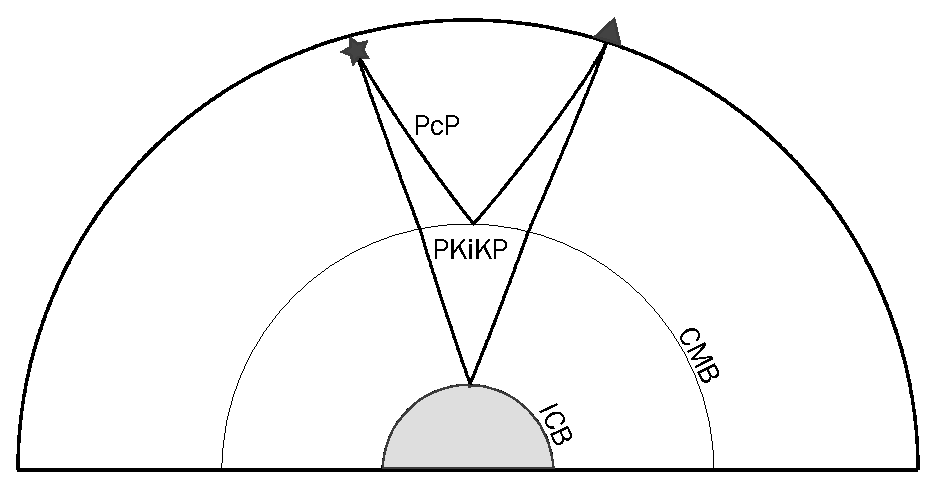
\includegraphics[width=0.7\linewidth]{fig/chap1/ray_path}
\caption{PcP和PKiKP射线路径示意图}
\label{fig:ray_path}
\end{figure}

\section{PKiKP/PcP振幅比的强烈离散}
作为内核冷凝增长和内核与外核相互作用的场所~\citep{Deguen2011,Bergman2010},地球的内外核边界(ICB)的物理性质一直也是地震学的重要问题之一. 到目前为止,对ICB的研究基本都是利用由该界面反射的PKiKP震相,而PKiKP也是内核存在最为直接的证据. PKiKP又分为前临界和后临界,在早期的观测条件下,后临界PKiKP(又被成为PKP${}_{df}$)的观测要更为容易,其作为参考震相,通常与PKP${}_{bc}$结合,被用于研究内
核顶部的结构~\citep{Tanaka1997}. 相比而言,由于较小的反射系数和较低的信噪比,加上观测条件的限制,
在早期对于小震中距情况下的前临界PKiKP的观测数量非常有限~\citep{Bolt1970},但还是有研究尝试利用PKiKP/PcP振幅比来估计内核的密度和ICB波速跃变~\citep{Souriau1989,Shearer1990}. 由于PcP和PKiKP在浅部结构中传播路径的相似性(图\ref{fig:ray_path}),这种使用振幅比的
方法假设可以消除地幔结构、台站响应等因素对观测结果的影响而且CMB是平坦且横向变化不大的,观测到振幅比异
常则来自内核,由此估计ICB的物理参数. \citet{Krasnoshchekov2005}用记录到核爆事件产生的PKiKP绝
对振幅来约束ICB的区域变化,推测出内核表面存在马赛克结构. 虽然振幅经过了震级校正,但台站的增益及场地效
应依然是不确定的因素. 因此,关于ICB的研究大多使用PcP作为参考震相. 随着近年来大规模地震台阵的安装和区
域性密集台网的布设,PKiKP的观测数量显著提升,通过搜索全球1995至2000年的IMS小口径台阵数据,利用叠加方法,\citet{Koper2004a}搜集了三百多个PKiKP观测,远远超过之前的观测数量的总和;利用Hi-net,\citet{Kawakatsu2006}首次报道了由一个地震产生的超过100个清晰的PKiKP记录,通过慢度分析和波形拟合,有
力地证实了尖锐ICB的存在. 虽然PKiKP的观测数量大大提升,但用它和PcP约束内核参数仍然面临很多困难. 首先
在小震中距情况下,PcP容易被S波的尾波干扰,因此限制了可用的数据量;其次,由于台阵口径有限,PKiKP在内核的反射有限,很难将所有采样区域的观测结果联系起来并结合地球动力学机制进行讨论~\citep{Tanaka2015a};再次,即使在很小的区域,观测到的振幅比也可能呈现出非常离散~\citep{Koper2004a},但造成数据离散
的来源却很难确定. 

大量观测表明内核并不是一个物性均一的刚性球体,除了波速的各向异性~\citep{Wang2015},现在也已有较多的
观测证据支持内核内部的不均匀性结构,像1-degree的东西半球的速度和衰减的不均匀~\citep{Tanaka1997,Wen2002}和内核顶部局部的小尺度散射结构~\citep{Vidale2000a}等. 一些地球动力学模型试图对这些结构的成因给出解释,如既有外核大尺度的非对称流~\citep{Aubert2008,Gubbins2011},也有来
自内核自身的内部对流~\citep{Alboussiere2010,Monnereau2010},但还没有一种模式能完全解释地震观
测. ICB是连接内外核的桥梁,因此可能对内核结构作出一定反映,因而一些最近的研究尝试将全球的PKiKP/PcP
振幅比和走时分布与内核的东西半球差异这种模式联系起来,但由于全球数据的离散,这种尝试看上去并不可行~\citep{Waszek2015a}. 

PKiKP/PcP振幅比和走时残差的区域性离散可能有多种来源. 其一,尽管PcP和PKiKP的离源
角相差不大,它们在的传播路径还是有一定差异,因此在地壳和地幔中的所经历的衰减和不均匀性结构也会有所不同,
从而贡献振幅比和走时差的异常~\citep{Tkalcic2010a};其二,由于PKiKP射线较PcP更陡,其受到横向结构
变化的影响较小,尤其是二者受震源附近和近台站下方的结构影响的差异;其三,也是本研究关注的主要内容,如前
面所述,CMB结构会不仅会造成PcP振幅的剧烈变化,其走时也会受到影响~\citep{Koper2003}. 然而,CMB对观
测的影响却很少被之前很多研究所提及或仅有少许讨论~\citep{Cao2004,Waszek2015a,Dai2012,Tanaka2015a}. 即使注意到了可能的CMB效应,使用之前的分析方法也很难将造成数据离散的来源确定~\citep{Koper2004a}. 除了以上因素,台站的信噪比条件同样不能忽视,因为PcP和PKiKP的到时不同,而两者被记录时的信噪比
环境也不相同. 综合上面的考虑,如果不能将每种来源小心地区分出来,用振幅比和走时残差的方法就很难得到真实
的ICB物理参数的估计. 

\section{本研究的主要工作}
由于短周期PcP(1--2Hz)对CMB结构变化敏感,能提供对该界面性质最直接的约束,且PKiKP 和PcP的振幅比呈现强烈离散,而异常可能源于CMB结构对PcP的影响,这就使得可以通过振幅比的变化推测CMB结构变化. 另外,以PKiKP作为参考震相,不仅可以减小由浅部结构产生的不确定性还可以有效判断引起PcP波形变化的来源. 因而利用PcP和PKiKP研究CMB结构变化存在很好的可行性,

本硕士论文的主要工作是首先通过收集全球IMS(International Miscellaneous Stations)小口径台阵记录到的PcP和PKiKP数据,从中筛选出产生同时被两个邻近小口径台阵记录到PKiKP和PcP信号的地震事件,这两个台阵的震中距也相近,通过对比两个台阵的观测包括PKiKP
和PcP的振幅比、走时残差和波形来确定产生区域性离散的PKiKP/PcP振幅比的来源;当没有两个相近震中距的相
邻台阵的时候,通过分析多个相邻地震产生的被同一台阵记录到的PKiKP和PcP信号,并结合前人的研究结果,来推
断观测异常的成因. 利用IMS小口径台阵,不仅可以提高观测的可靠性,得出对于某个台阵的平均振幅比,以此有效
评估台阵观测的可信度,而且经过对不同台阵、地震事件和震相的比较后,一些可能对观测造成影响的因素可以被排
除,并且确认CMB的界面起伏变化和低速结构可以基本上解释PKiKP/PcP振幅比在小尺度范围内的强烈离散以及PcP的
变化. 虽然研究使用的还是常规的走时和振幅分析方法,但通过运用以上对比方法,有效地改善了对CMB小尺度结构
的分辨能力. 除了IMS小口径台阵的观测,本研究还补充了国家测震台网的数据,利用大规模的采样来分析大尺度范围内的CMB结构变化. 为了评价单台站的观测结果和分析不确定性的来源,本研究还对重复地震的PKiKP和PcP数据进行了分析和比较. 最后,尝试将本研究的观测结果和之前的地球动力学模拟结合起来,简要讨论CMB各种变化的形成机制. 

\chapter{数据和方法}

本研究尝试利用PcP-PKiKP震相组合来探测核幔边界的小尺度结构,包括界面起伏变化和其上方的速度异常,因此需要同时用到这两个震相的振幅和走时信息. CMB的起伏主要通过与标准模型的走时残差来约束,而其物性变化主要依靠PKiKP/PcP的振幅比来推断. 获得这两种信息都需要观测记录上出现可识别的震相,然而在一道地震记录上同时观测到PcP和PKiKP信号是比较困难的. 首先,对于PKiKP,由于较小的反射系数(图\ref{fig:rtf}b)加之噪声的干扰,其观测难度要远大于常规的核震相;其次,能观测到清晰PcP震相的震中距常常比较有限,在小震中距情况下,PcP的反射系数较小(图\ref{fig:rtf}a),而且容易受到S波及其尾波的干扰,因此比较合适的观测区间大致位于30{\textdegree}--40{\textdegree}. 因此,采用台阵叠加方法寻找和识别弱信号则非常有必要. 本章主要介绍研究所用到的数据来源、全球的PKiKP和PcP观测情况,以及包括PWS在内的数据处理方法和振幅比、走时残差测量和可靠性评价方法. 


\begin{figure}[!ht]
		\centering
%		\subfloat[][]{\label{fig:cmb}%
%		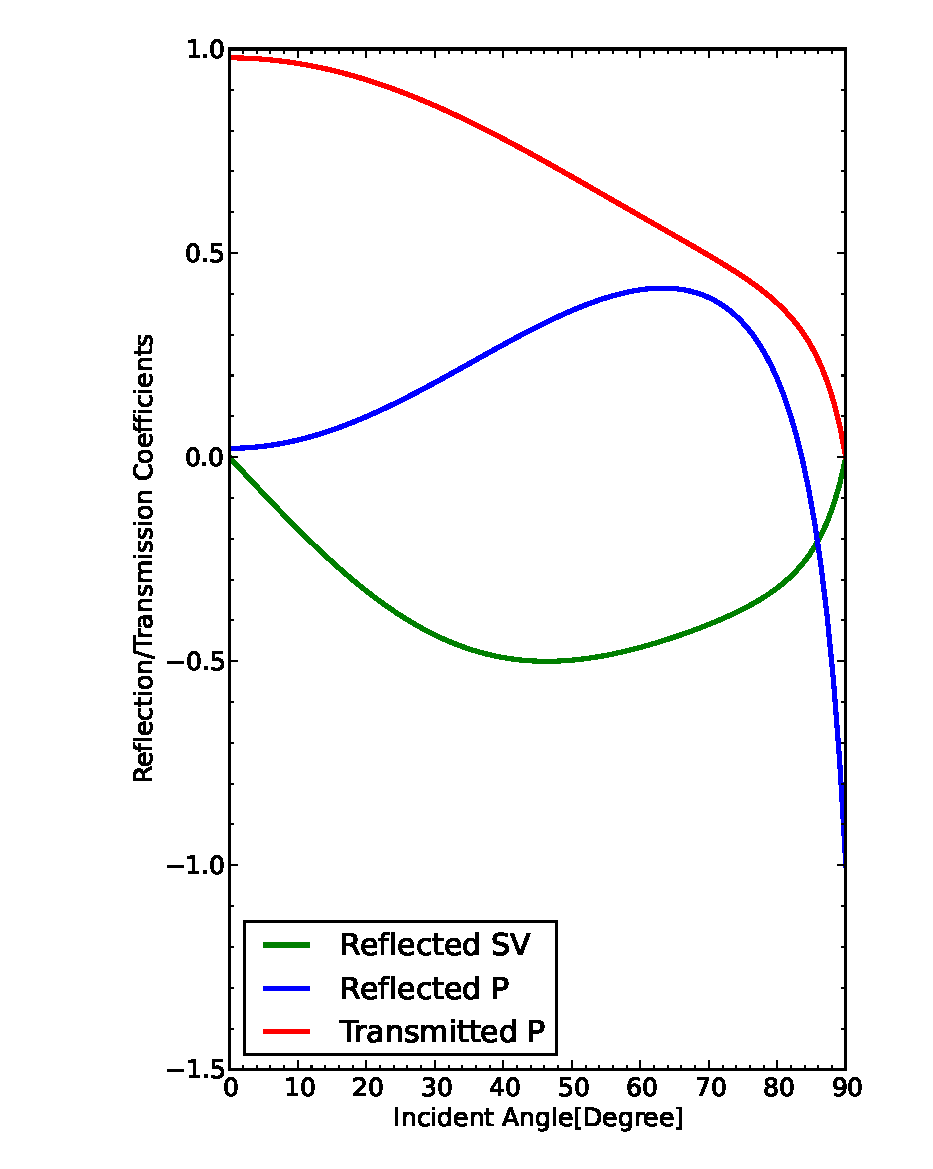
\includegraphics[width=0.45\linewidth]{fig/chap2/cmb.eps}
%}			
%		%\hspace{2em}
%		\subfloat[][]{\label{fig:icb}%
%		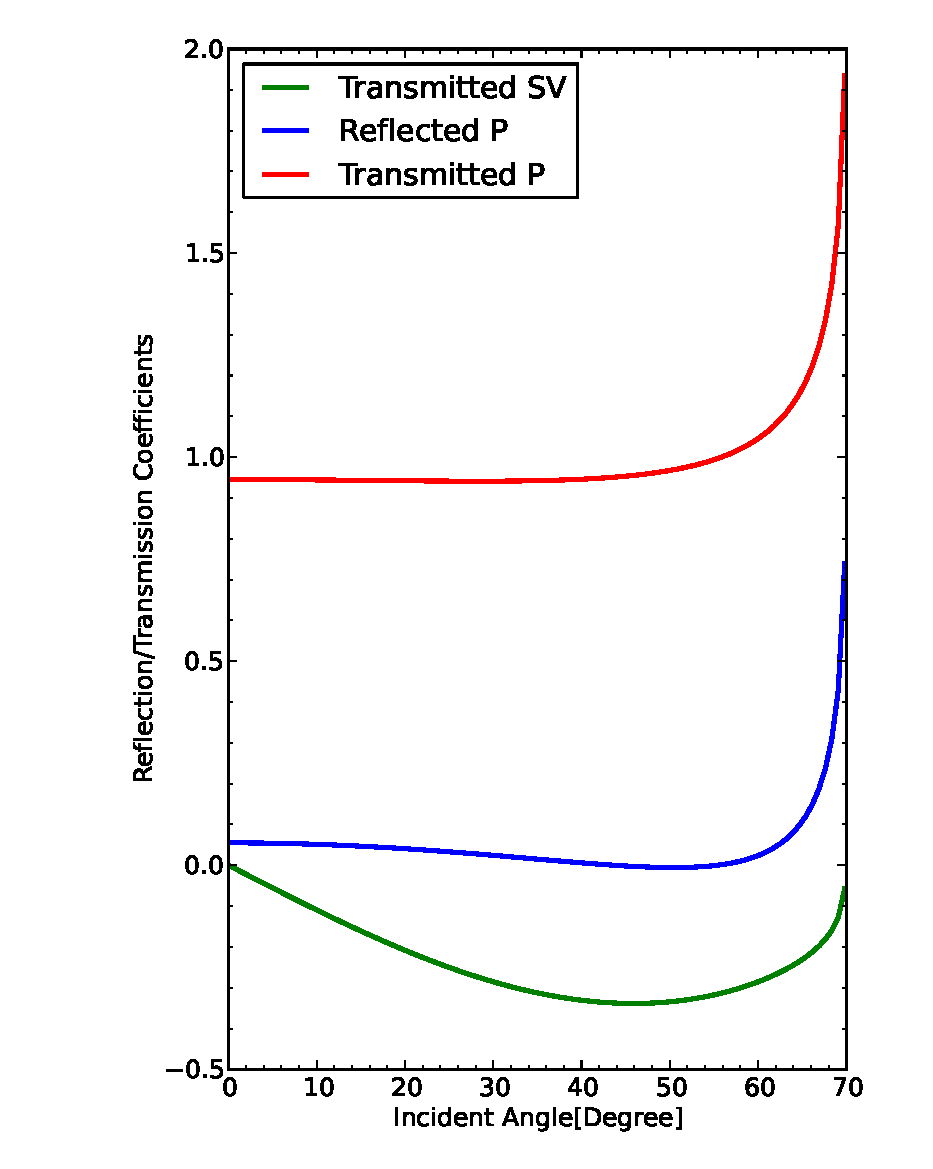
\includegraphics[width=0.45\linewidth]{fig/chap2/icb.eps}
%}		
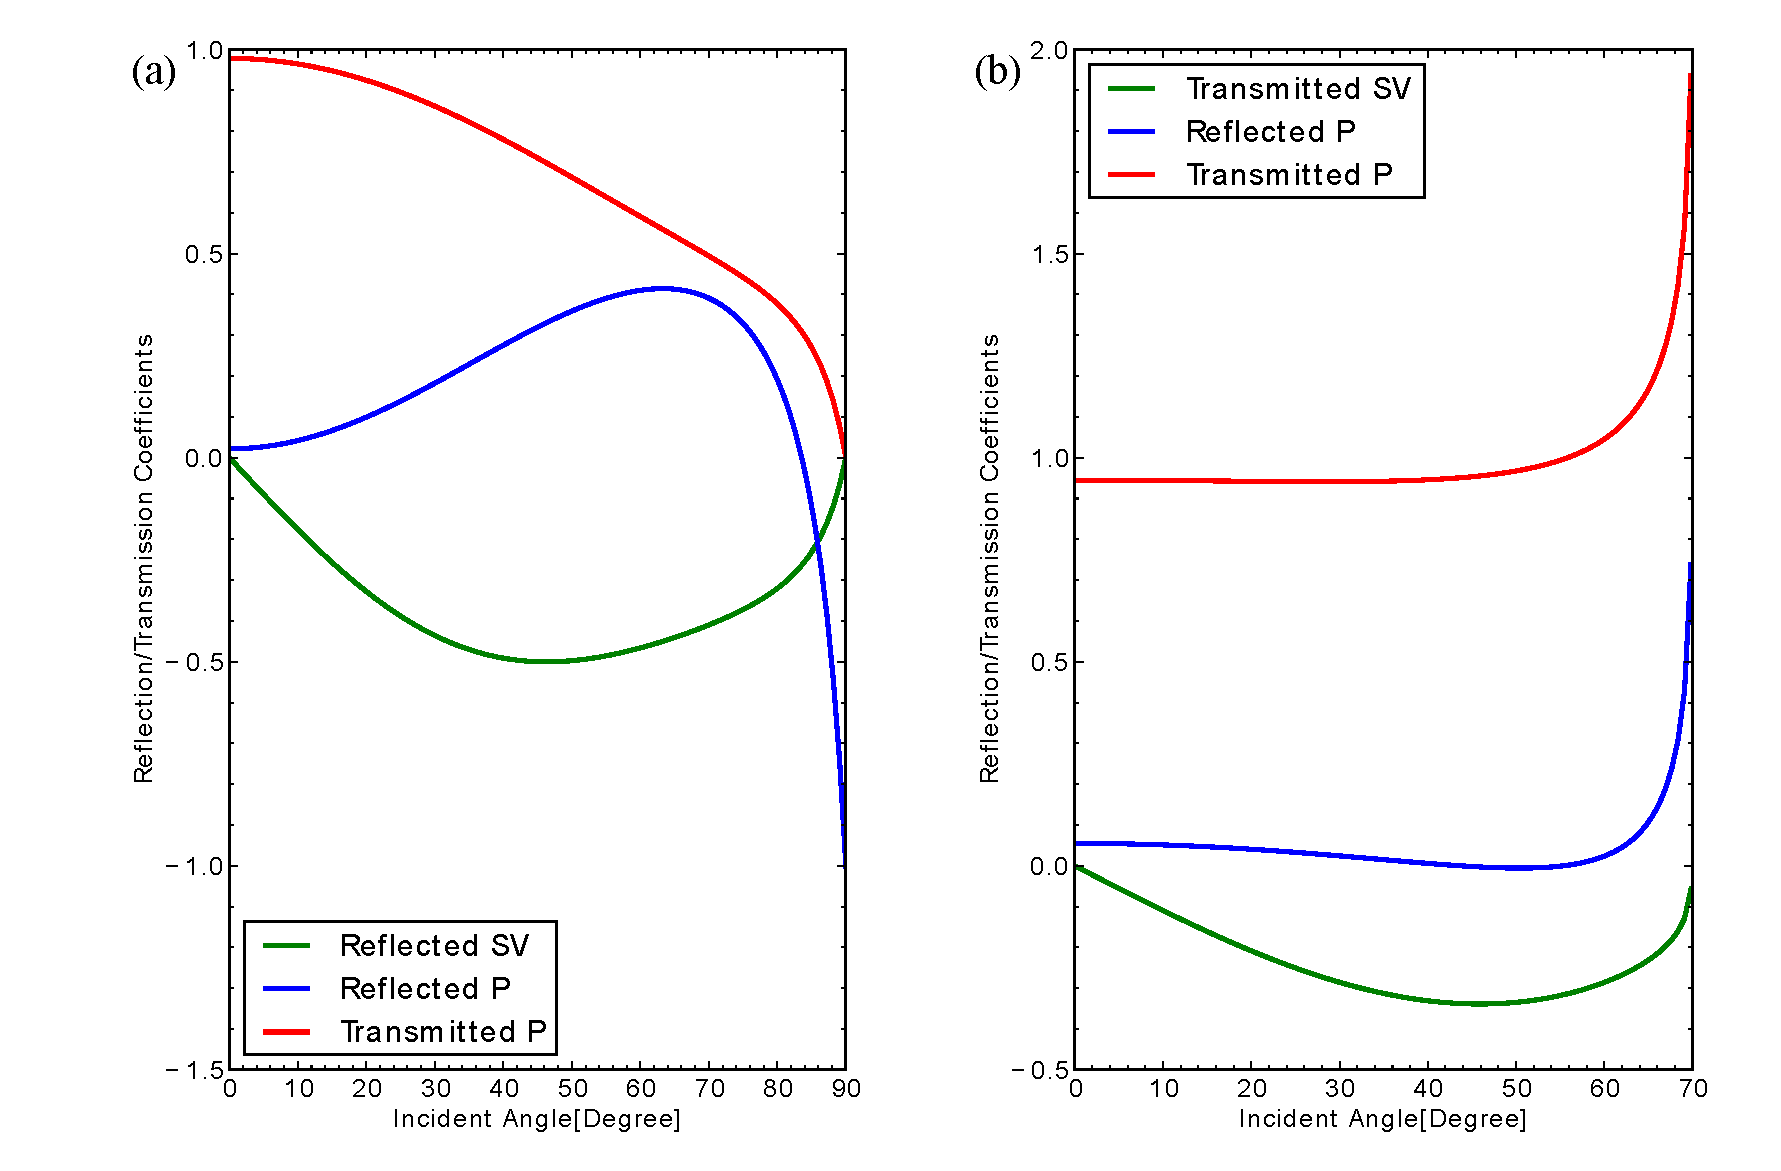
\includegraphics[width=0.9\linewidth]{fig/chap2/cmb_icb.eps}
		\caption{根据PREM计算的(a)~CMB和(b)~ICB 的P波反射、透射系数. 与透射和转换P波系数相比,PKiKP的反射系数非常小;而PcP反射系数大约在入射角为60{\textdegree}左右时取得最大. }
		\label{fig:rtf}
\end{figure}


\section{数据来源}

本硕士论文的前期工作主要是在全球范围内寻找PKiKP震相,然后从观测到PKiKP信号的地震记录中挑选出含有可识别PcP信号的记录. 数据的来源有(1)在IRIS上可下载的全球IMS小口径台阵数据;(2)日本Hi-net台网;(3)
国家测震台网,数据从国家测震台网数据备份中心(State Earthquake Information Service-Data Management Center)得到;(4)美国USArray. 数据来源的具体分布见图\ref{fig:data_source},可以看出由于台站分布的南北不均匀性,南半球的CMB和ICB的采样较少,只有澳大利用几个小口径台阵的数据. 

\begin{figure}
\centering
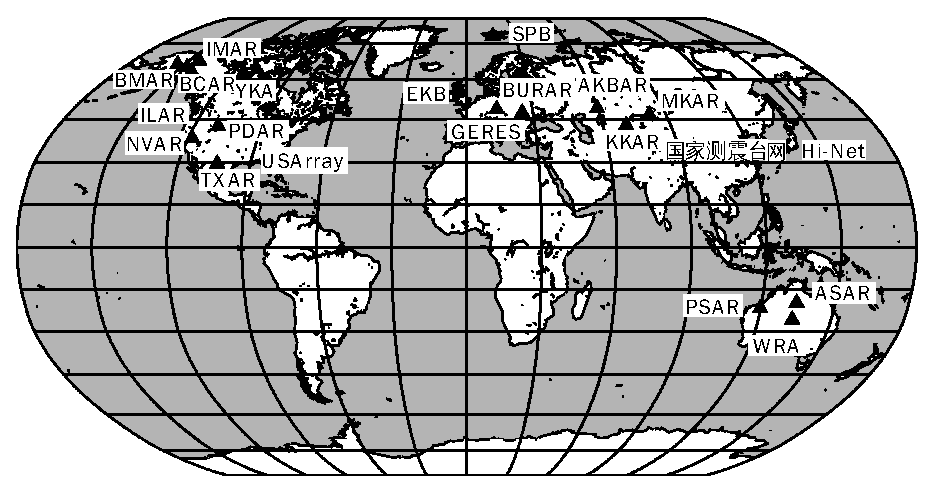
\includegraphics[width=0.8\linewidth]{fig/chap2/data_source}
\caption{本研究所收集PKiKP和PcP观测记录的数据来源分布. 包括全球范围分布的IMS小口径台阵,还有国家测震台网等大型密集台网. }
\label{fig:data_source}
\end{figure}

\subsection{IMS小口径台阵}

对于IMS小口径台阵,IRIS上大部分可下载数据的时间范围从2000至2015年,因此搜索的地震事件也基本在这个
时间范围,数据并不与之前的研究重合~\citep{Koper2004a}. 筛选的地震事件震级均大于Mw5.0,以保
证能产生可观测的PKiKP信号;地震的深度不加限制,因为IMS均为用于核爆监测目的的短周期台站,PKiKP
记录并不会受到浅源地震产生的面波的显著干扰;震中距范围从10{\textdegree}--50{\textdegree}. 利用IMS台阵数据做对比分析是本研究的主要内容,但从全球范围来看适合的台阵对并不多. 首先,台阵的分布很
不均匀,目前半数都位于北美,包括阿拉斯加的BCAR,BMAR,IMAR和ILAR;加拿大的Yellow Knife(YKA);
美国的NVAR,PDAR和TXAR. 而要满足相近震中距条件,再加上地震位置的限制,使得能够用来进行对照分析的台
阵组合仅有阿拉斯加的四个小口径台阵,美国的PDAR-NVAR和澳大利亚的WRA-ASAR. 位于中亚和欧洲的台阵有的没有
与之成对的台阵;有些由于震中距比较大(>50{\textdegree})和较低的信噪比,不能同时记录到同一地震事件
产生的PKiKP和PcP信号. 因此,本文集中讨论北美和澳大利亚IMS台阵的观测. 

\begin{table}[ht]
	\centering
	\caption{本文搜集PcP和PKiKP所用到的IMS小口径台阵}
	\begin{tabular}{*{5}{c}}
\hline
台阵 & 台站数 & 纬度\textsuperscript{*}(\textdegree) & 经度\textsuperscript{*}(\textdegree) & 数据起止日期\\
\hline
AKBAR & 9 & 49.2 & 59.9 & 2003.12--2015.09\\
MKAR & 10 & 46.7 & 82.3 & 2000.09--2015.09\\
KKAR & 9 & 43.1 & 70.5 & 2001.12--2015.09\\
BCAR & 5 & 63.0 & -141.8 & 2013.11--\\
BMAR & 5 & 67.4 & -144.5 & 2013.11--\\
IMAR & 5 & 66.0 & -153.7 & 2013.11--\\
ILAR & 19 & 64.7 & -146.9 & 1998.03--\\
YKA & 18 & 62.5 & -114.6 & 2005.09--\\
NVAR & 11 & 38.4 & -118.3 & 2003.07--\\
PDAR & 14 & 42.7 & -109.5 & 1998.03--\\
TXAR & 10 & 23.3 & -103.6 & 2000.04--\\
GERES & 24 & 48.8 & 13.7 & 2001.08--2002.03\\
BURAR & 9 & 47.6 & 25.2 & 2007.09--\\
EKB & 21 & -3.1 & 55.3 & 2014.03--\\
WRA & 26 & -19.9 & 134.4 & 2005.01--\\
ASAR & 19 & -23.6 & 133.9 & 2003.08--\\
PSAR & 13 & -21.5 & 119.8 & 2011.01--\\
SPB & 5 & 78.1 & 16.3 & 2009.03--\\
\hline
\multicolumn{5}{l}{\textsuperscript{*}\footnotesize{台阵的经纬度仅保留至一位小数}}
	\end{tabular}
\label{array}
\end{table}

每个IMS台阵基本由10到25个短周期台站组成(表\ref{array}),但有几个台阵例外,例如BCAR,BMAR和IMAR,它们在IRIS上的可用数据只从2013年才开始,尽管如此,它们也能为本研究补充一定的PcP和PKiKP观测. 
从所有可用数据中一共找到300个观测到PKiKP信号的台阵-事件对,从数据的分布来看,PKiKP观测集中在北美和澳大利亚区域,中亚和欧洲台阵的观测比较稀疏,这也和这些区域地震活动性不强有关(图\ref{fig:gl_pkikp}),从这些数据中再进行挑选得到同时观测到PcP和PKiKP的仅127对. 即使搜索了超过一万个地震的的数据,所找到的有效PKiKP数量仍然不多,这也表现出PKiKP弱振幅的本质并且其可观测性强烈依赖于环境噪声和台站状态. 尽管如此,利用这些小口径台阵还是能得到很多高质量的PcP和PKiKP观测,即不用做任何额外处理即可在全部台站的记录上看到这两个信号.

\begin{figure}
\centering
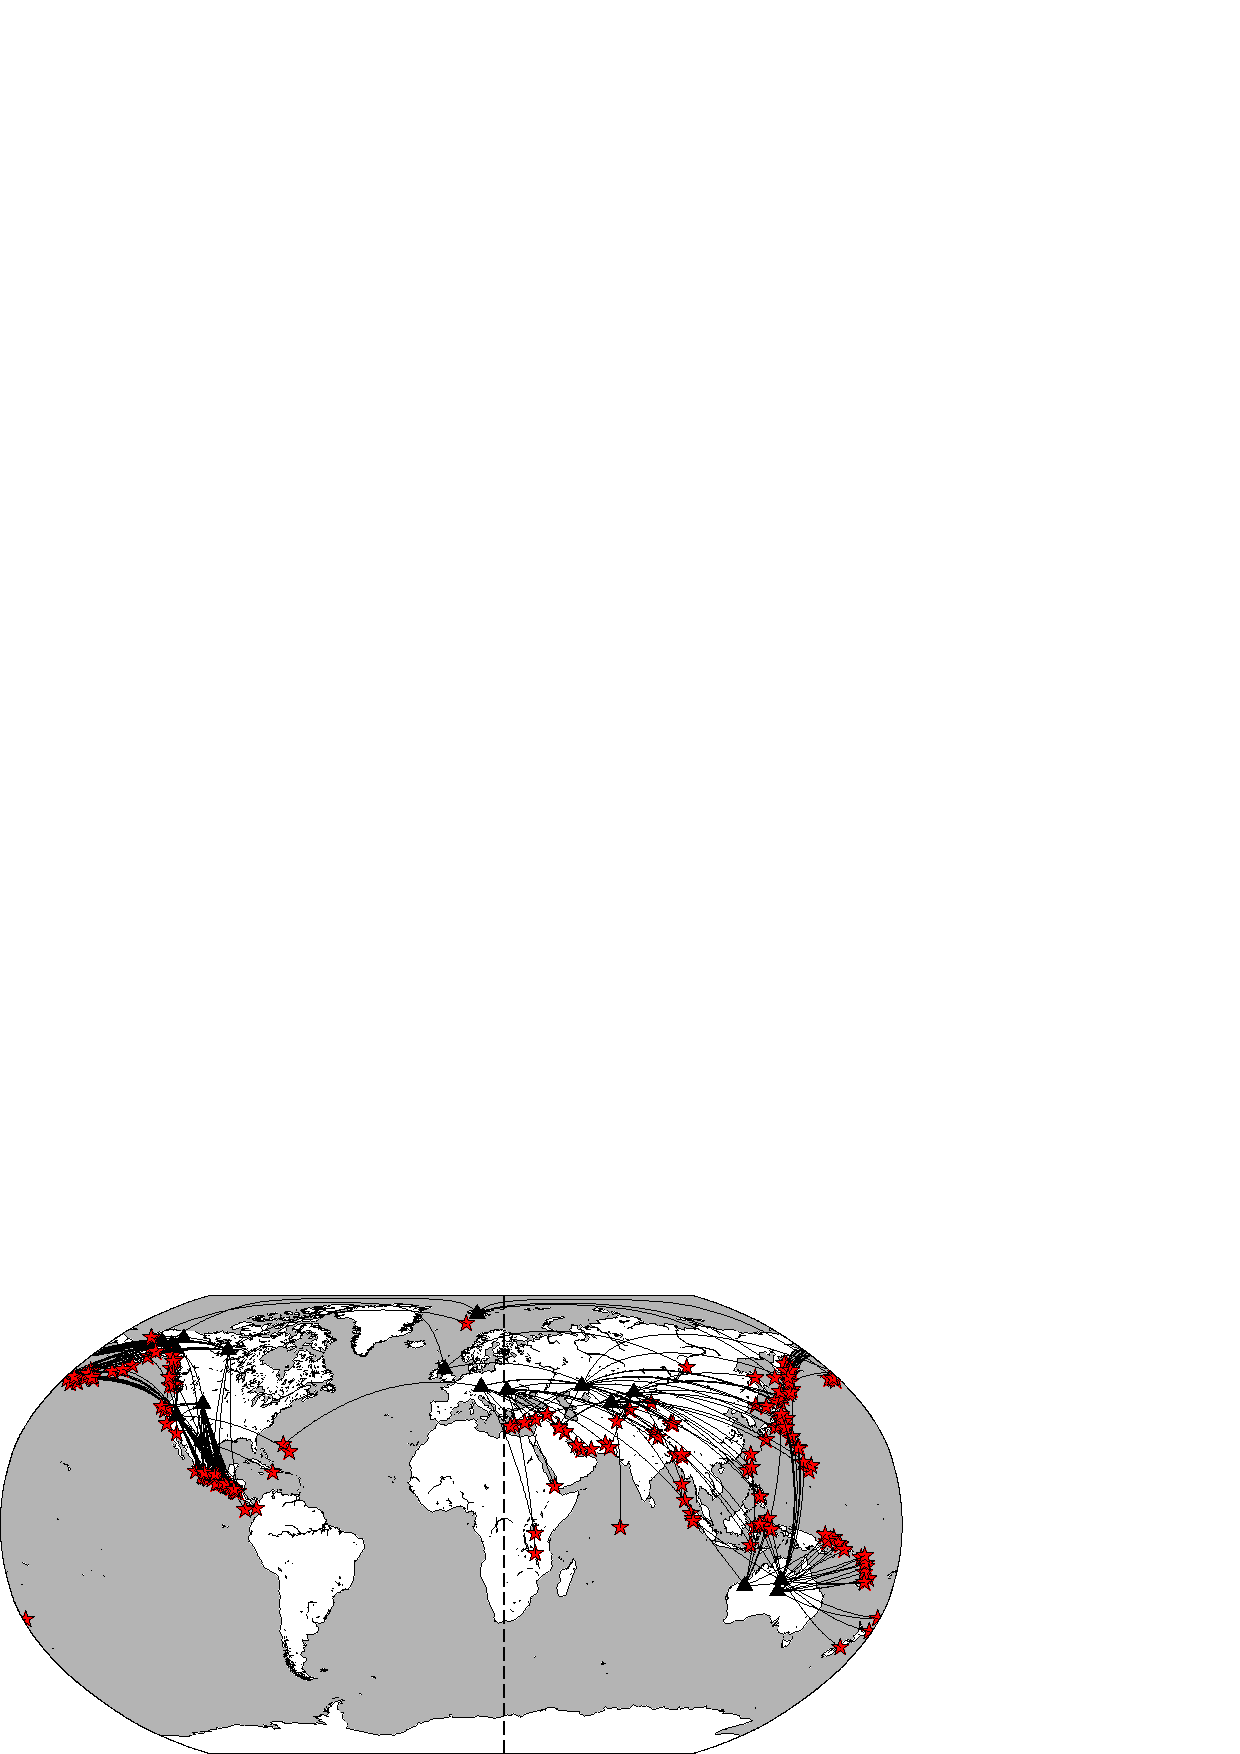
\includegraphics[width=0.8\linewidth]{fig/chap2/gl_pkikp}
\caption{利用全球IMS小口径台阵获得了300对可观测到PKiKP信号的事件-台阵对. 虚线为~\citet{Tanaka1997}定义的准东西半球分界线. 红色五角星为地震,黑色三角形表示IMS台阵. }
\label{fig:gl_pkikp}
\end{figure}

\begin{figure}
\centering
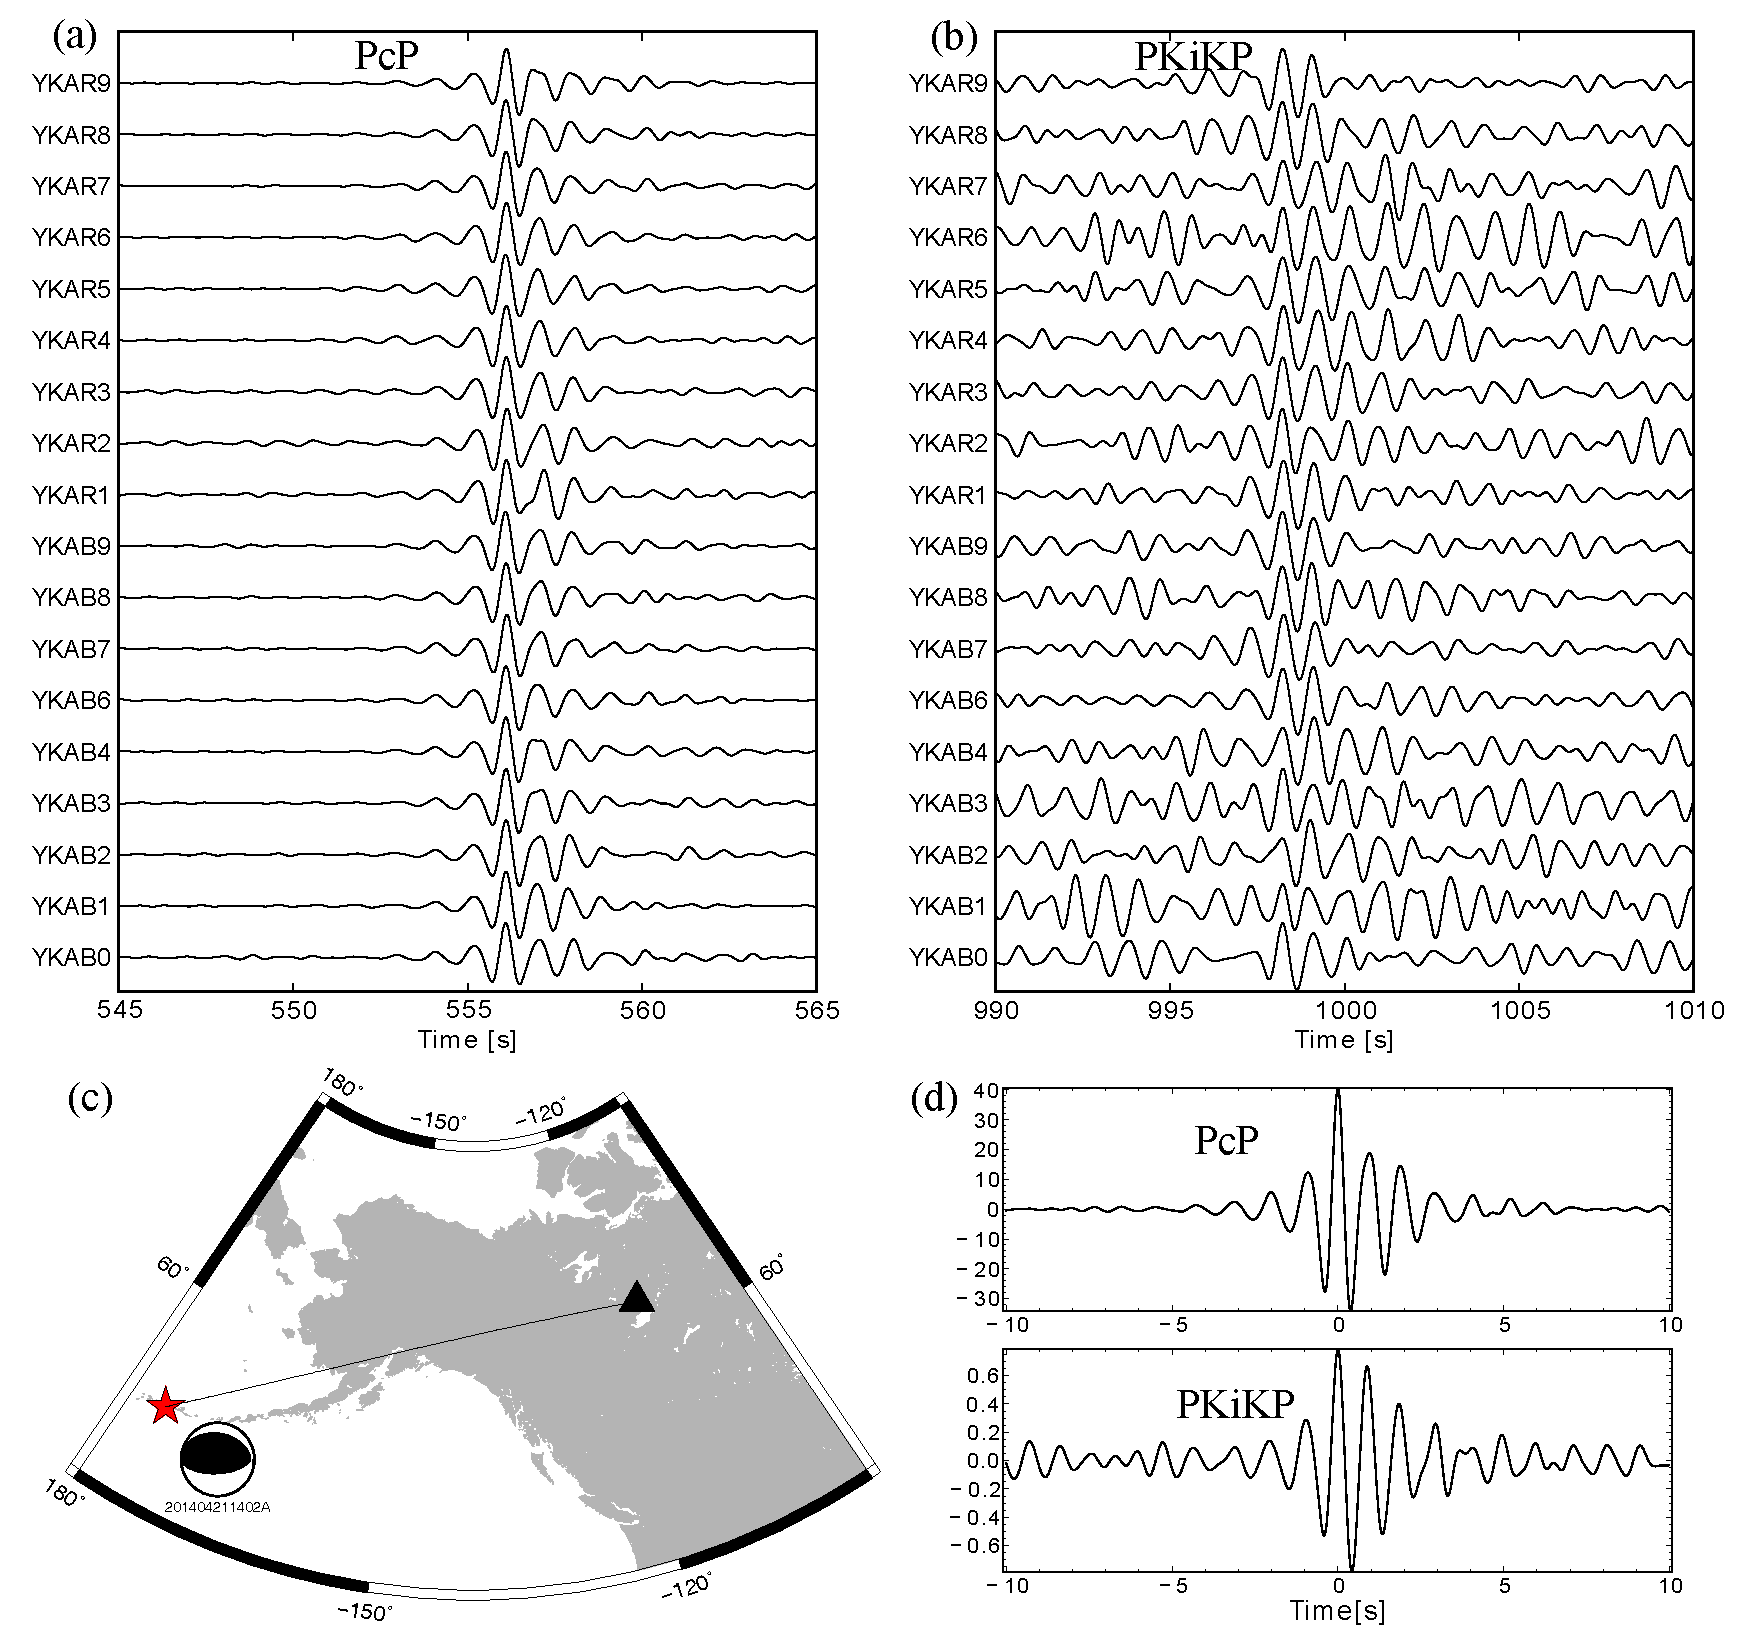
\includegraphics[width=\linewidth]{fig/chap2/4599655_yka}
\caption{YKA记录到的表\ref{evt}中事件10产生的PcP和PKiKP信号. (a) PcP;(b) PKiKP;(c)地震和台阵位置;(d) 按波峰对齐叠加后的PcP和PKiKP波形. }
\label{fig:4599655_yka}
\end{figure}

\begin{figure}
\centering
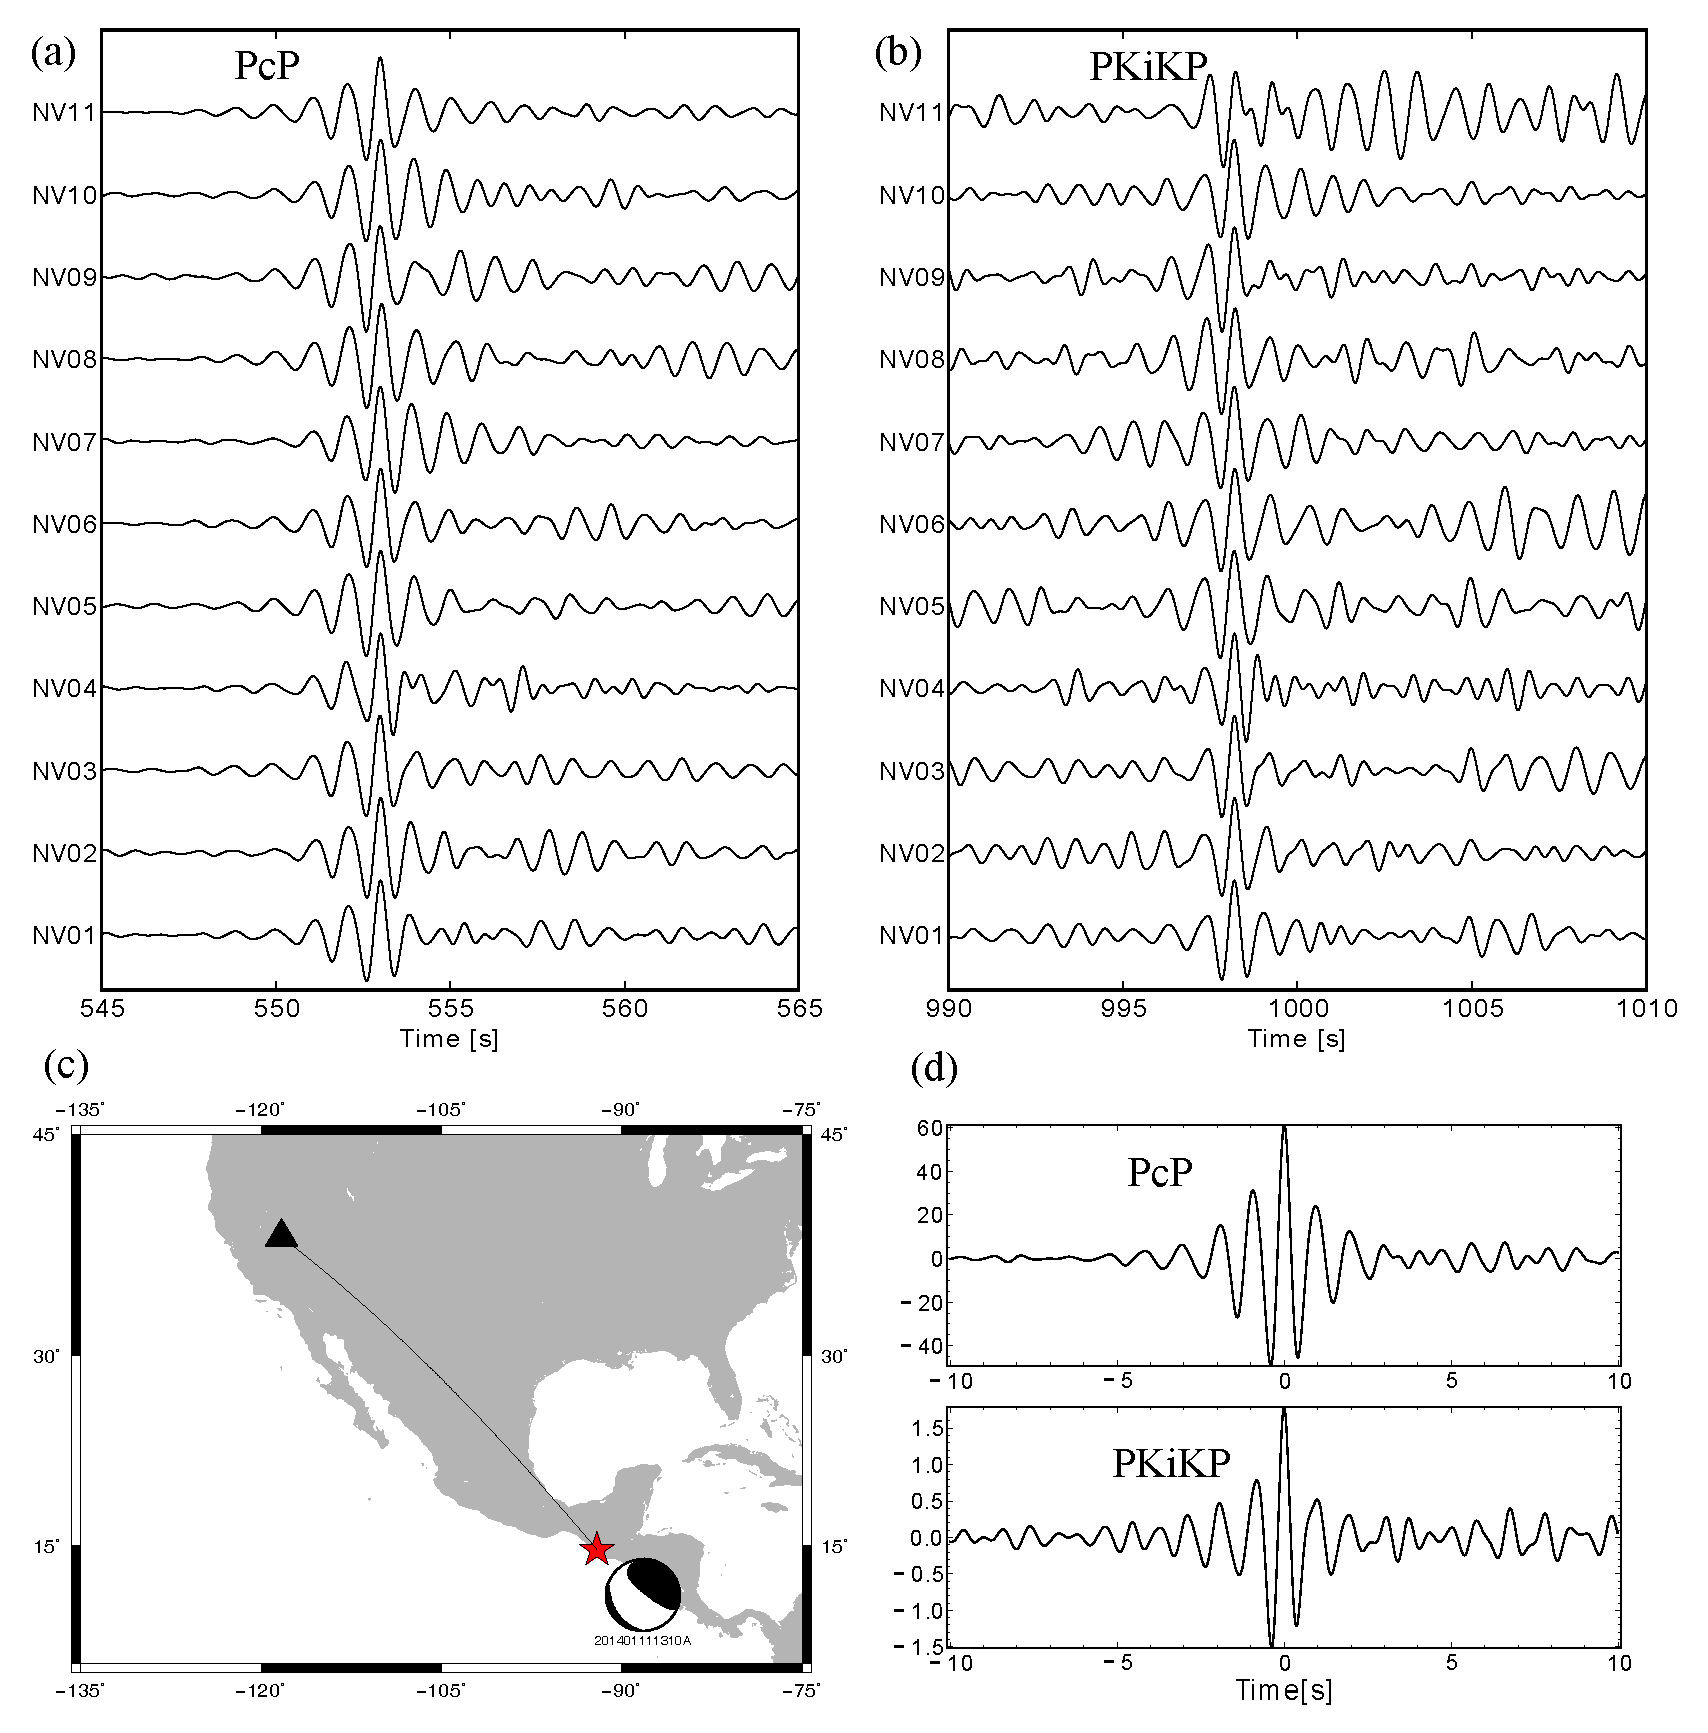
\includegraphics[width=1\linewidth]{fig/chap2/4371355_nvar}
\caption{NVAR记录到的表\ref{evt}中事件15产生的PcP和PKiKP信号. (a) PcP;(b) PKiKP;(c)地震和台阵位置;(d) 按波峰对齐叠加后的PcP和PKiKP波形. }
\label{fig:4371355_nvar}
\end{figure}

\begin{figure}
\centering
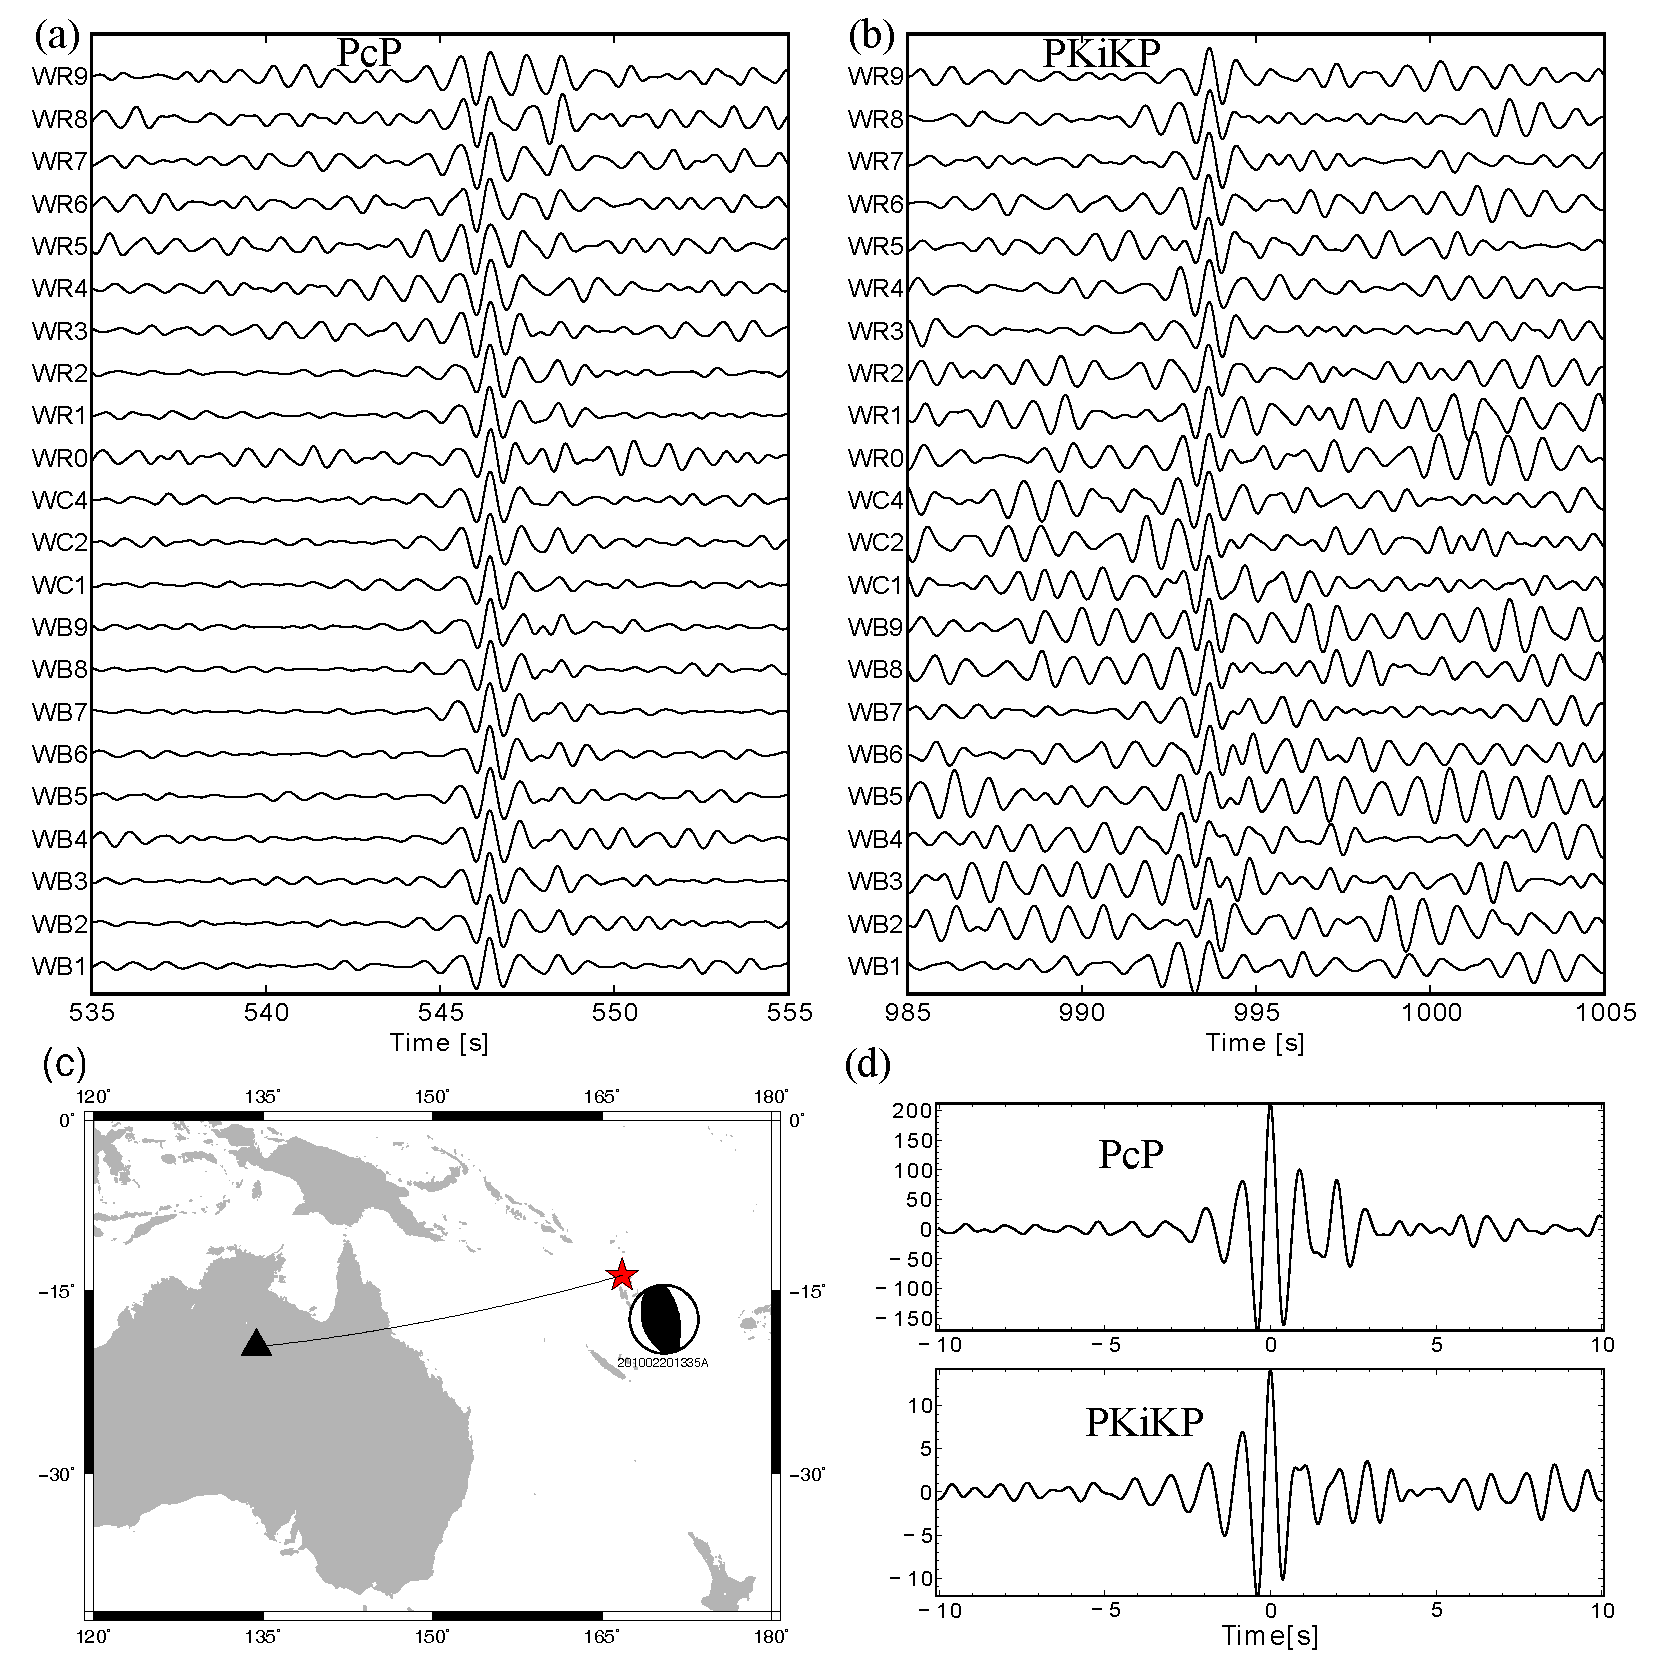
\includegraphics[width=1\linewidth]{fig/chap2/2844731_wra}
\caption{WRA记录到的表\ref{evt}中事件18产生的PcP和PKiKP信号. (a) PcP;(b) PKiKP;(c)地震和台阵位置;(d) 按波峰对齐叠加后的PcP和PKiKP波形. }
\label{fig:2844731_wra}
\end{figure}


由于IMS台阵的口径很小(一般为20km左右),每个台阵的台间距仅有几千米,因此可以减小单一台站产生的不确定性,比如由台站场地效应或者接收端下方的不均匀性造成的PcP和PKiKP振幅变化,并可以得到有效的观测质量评
价. 同时对PKiKP这样的弱震相的观测也将更加的可信,因为可以通过台阵叠加技术增加信噪比,对弱信号进行确认
,排除随机噪声的可能性~\citep{Rost2002},这一点将在后面进行详细叙述. 对所有的IMS数据,都经过去除仪器响应,并进行1--2Hz的四极Butterworth带通滤波. 根据前人的研究,这个频率范围是比较适合同时观测到PcP和PKiKP信号的~\citep{Koper2004a,Poupinet2004}. 在127个观测到PKiKP和PcP信号的地震之中,被两个台阵同时记录到这两个信号,且具有相近震中距情况的的只有30个左右,其中10个由NVAR和PDAR记录到(表\ref{evt},No.1--10);被WRA和ASAR记录的也有6个(表\ref{evt},No.17--23). 本文因此集中对这些地震的PKiKP和PcP数据进行分析. 

除了被两个台阵同时记录到的PcP和PKiKP数据,本研究还使用到了7个相邻地震产生的被同一个YKA台阵记录到的
PcP和PKiKP信号进行分析,来验证~\citet{Rost2004a}报道的阿拉斯加Kenai半岛下方CMB凹陷对PcP的放大效应. 这七个地震均位于阿留申群岛(表\ref{evt},No.11--17),与之前研究采样到相似的CMB区域. 

\begin{table}[ht]
	\centering
	\caption{本研究的对照分析所用到的所有地震.}
	\begin{tabular}{*{7}{c}}
	\hline
	事件号 & 日期 & 时间 & 纬度(\textdegree) & 经度(\textdegree) & 深度 & 震级(Mw)\\
	\hline
1 & 2003/08/25 & 06:28:34.9 &  13.9932 &  -91.1255 &  99.5 & 5.9\\
2 & 2007/07/23 & 22:30:09.2 &  14.465  &  -90.906  &  115  & 5.5\\
3 & 2009/11/26 & 19:08:10.4 &  13.4767 &  -89.9617 &  48.5 & 5.9\\
4 & 2009/04/27 & 16:46:27.5 &  16.9557 &  -99.5717 &  31.7 & 5.8\\
5 & 2009/05/03 & 16:21:46.4 &  14.6199 &  -91.2025 &  113.9 & 6.3\\
6 & 2009/08/15 & 13:22:43.1 &  18.0998 & -100.6157 &  61.2 & 5.5\\
7 & 2012/06/27 & 06:30:59.8 &  13.834  &  -89.967  &  132.6 & 5.7\\
8 & 2012/11/15 & 09:20:21.9 &  18.346  & -100.382  &  53  & 6.1\\
9 & 2013/07/08 & 02:52:42.6 &  13.2316 &  -89.1292 &  55  & 5.7\\
10 & 2014/01/11 & 13:10:51.1 &  14.6437 &  -92.0592 &  78  & 5.5\\
11 & 2015/04/23 & 14:57:27.7 &  51.7501 &  176.3353 &  31  & 5.3\\
12 & 2015/01/18 & 04:47:38.0 &  51.9238 &  179.578  &  102  & 5.5\\
13 & 2014/03/25 & 17:37:48.4 &  52.5754 & -177.1562 &  210.8 & 5.2\\
14 & 2007/07/13 & 21:54:44.9 &  51.904  & -176.2683 &  46.1 & 6.0\\
15 & 2014/04/21 & 14:02:15.8 &  51.844  & -175.9782 &  54.2 & 5.4\\
16 & 2009/04/21 & 08:37:28.8 &  52.2147 & -173.3826 &  68.3 & 5.2\\
17 & 2009/01/26 & 19:11:48.2 &  52.0884 & -171.3288 &  32.9 & 5.7\\
18 & 2010/02/20 & 13:35:57.1 & -13.6853 &  166.7666 &  87.3 & 5.5\\
19 & 2010/06/17 & 13:06:51.3 & -33.1905 &  179.7819 &  211.2 & 6.0\\
20 & 2011/01/26 & 17:03:30.1 & -11.0379 &  166.3601 &  153.5 & 5.8\\
21 & 2007/08/19 & 13:44:06.0 & -20.6189 &  169.7323 &  89.7 & 5.6\\
22 & 2007/11/20 & 15:28:28.6 & -29.973  & -177.9397 &  57.8 & 5.9\\
23 & 2007/10/11 & 05:31:55.6 & -18.5046 &  168.991  &  214  & 5.4\\
	\hline
\multicolumn{7}{l}{\footnotesize{注:1--10,11-17和18-23号事件分别用于后面三个区域的分析.}}
\end{tabular}
\label{evt}
\end{table}

\subsection{大型台网}

本研究还利用全球现有的大型台网增大PKiKP和PcP的观测数量,以此补充IMS小口径台阵的数据并增大采样区域,试图探索大尺度下的CMB或者ICB变化. 对于北美的NVAR和PDAR,它们记录到表\ref{evt}中地震2和3的时刻,美国的流动台网USArray恰好分别移动到这两个台阵附近,这样就提供了一个很好的机会比较两个数据集,进一步验证IMS台阵的观测结果. 虽然USArray台站的信噪比不如IMS台阵,但仍然有一些清晰的PKiKP和PcP观测. 

\begin{figure}[ht]
		\centering
		\subfloat[PKiKP]{\label{pkikp11}%
		\includegraphics[width=0.45\linewidth,height=0.4\textheight]{fig/chap2/pkikp_sec_2011.eps}
		}
		%\hspace{1em}
		\subfloat[PcP]{\label{pcp11}%
		\includegraphics[width=0.45\linewidth,height=0.4\textheight]{fig/chap2/pcp_sec_2011.eps}
		}
		\caption{国家测震台网记录到的事件2011/02/04 13:53:46(Dep=86km,Mw6.3)产生的549道单道可见的PKiKP\subref{pkikp11}信号,对应的PcP\subref{pcp11}也比较明显,但在某些区段看不到PcP信号. }
		\label{cn_2011}
\end{figure}


\begin{figure}
\centering
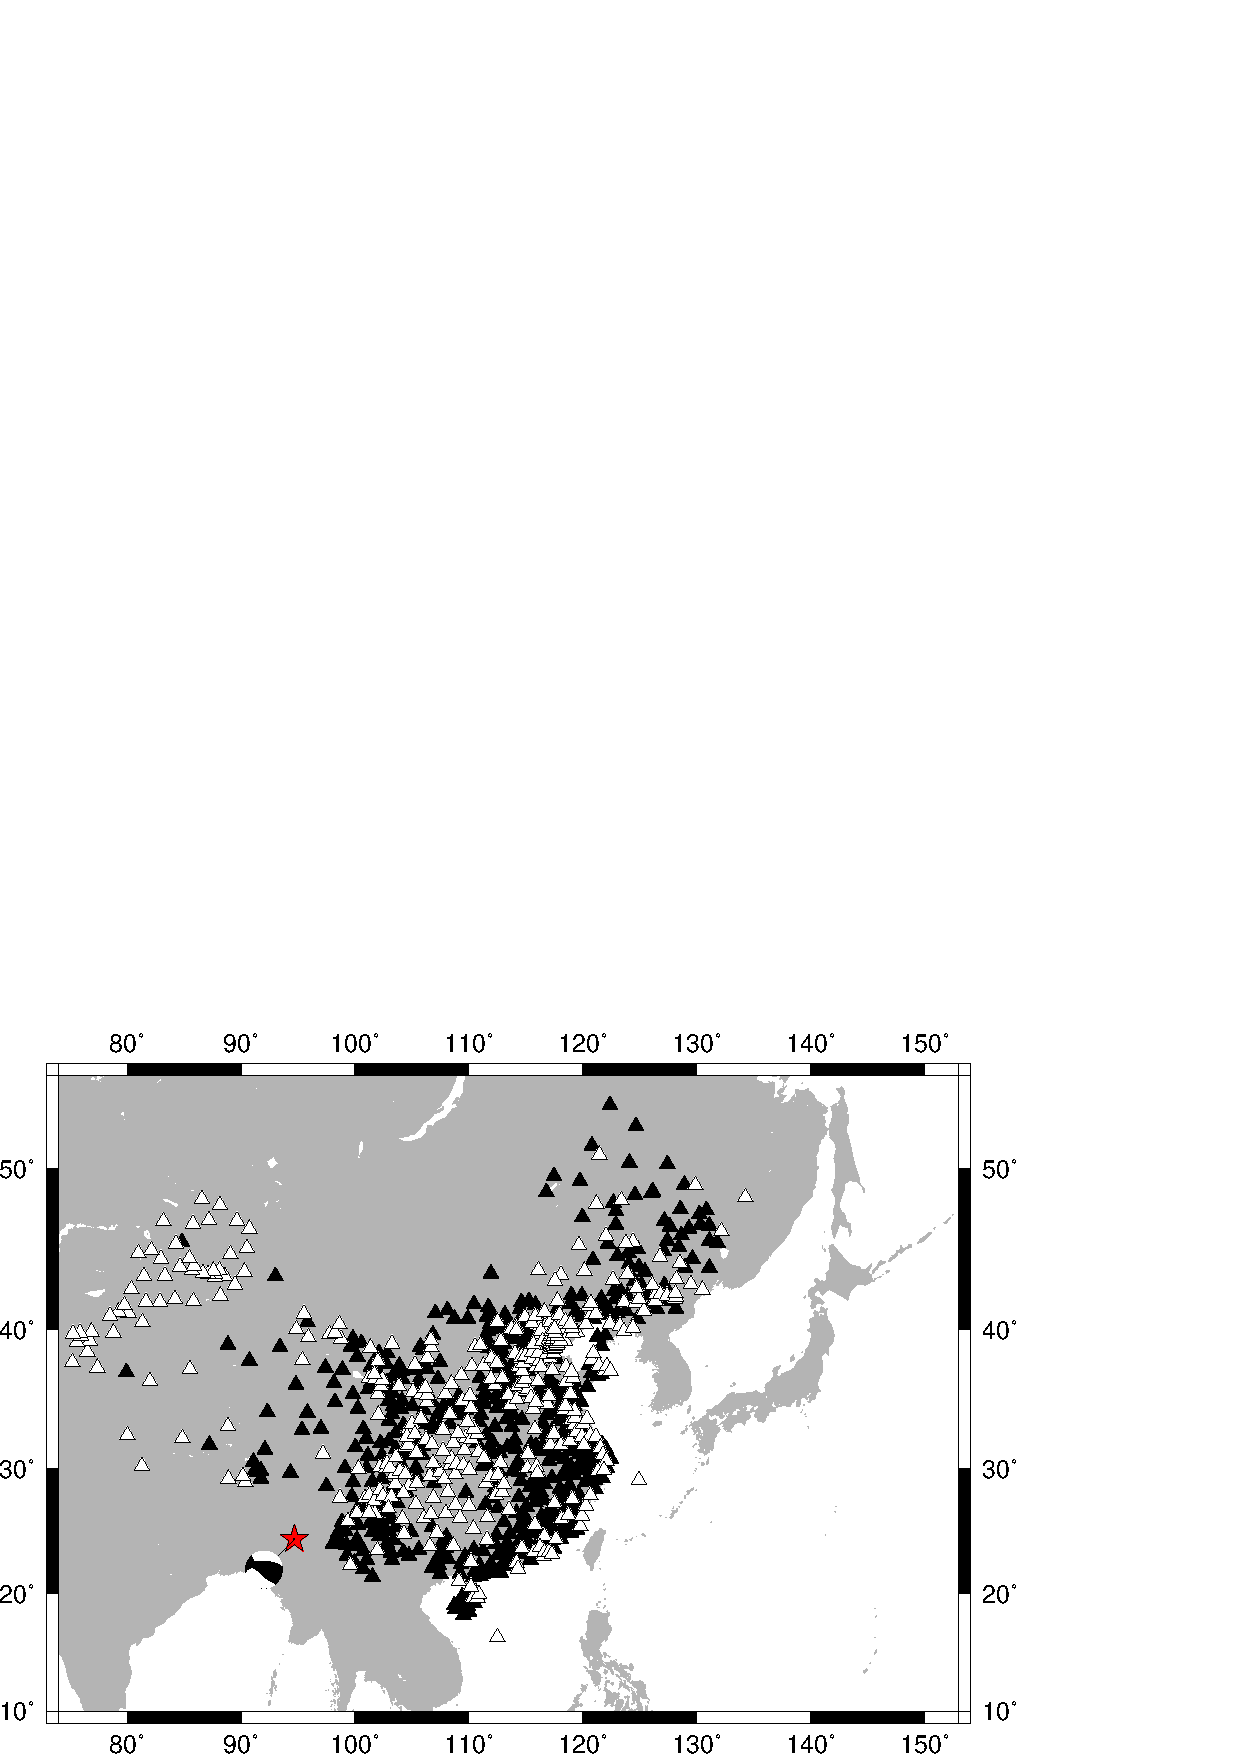
\includegraphics[width=0.8\linewidth]{fig/chap2/ev_sta_2011}
\caption{图\ref{cn_2011}中记录对应的台阵分布和地震位置. 黑色三角形表示记录到PKiKP信号的台站,白色的表示未记录到PKiKP信号的台站.}
\label{fig:ev_sta_2011}
\end{figure}


\begin{figure}[ht]
		\centering
		\subfloat[PKiKP]{\label{pkikp13}%
		\includegraphics[width=0.45\linewidth,height=0.4\textheight]{fig/chap2/pkikp_sec_2013.eps}
		}
		%\hspace{1em}
		\subfloat[PcP]{\label{pcp13}%
		\includegraphics[width=0.45\linewidth,height=0.4\textheight]{fig/chap2/pcp_sec_2013.eps}
		}
		\caption{国家测震台网记录到的事件2013/05/24 14:56:30(Dep=630km,Mw6.7)产生的513道单道可见的PKiKP\subref{pkikp13}信号,对应的PcP\subref{pcp13}也比较明显,但在某些区段看不到PcP信号. }
		\label{cn_2013}
\end{figure}


\begin{figure}
\centering
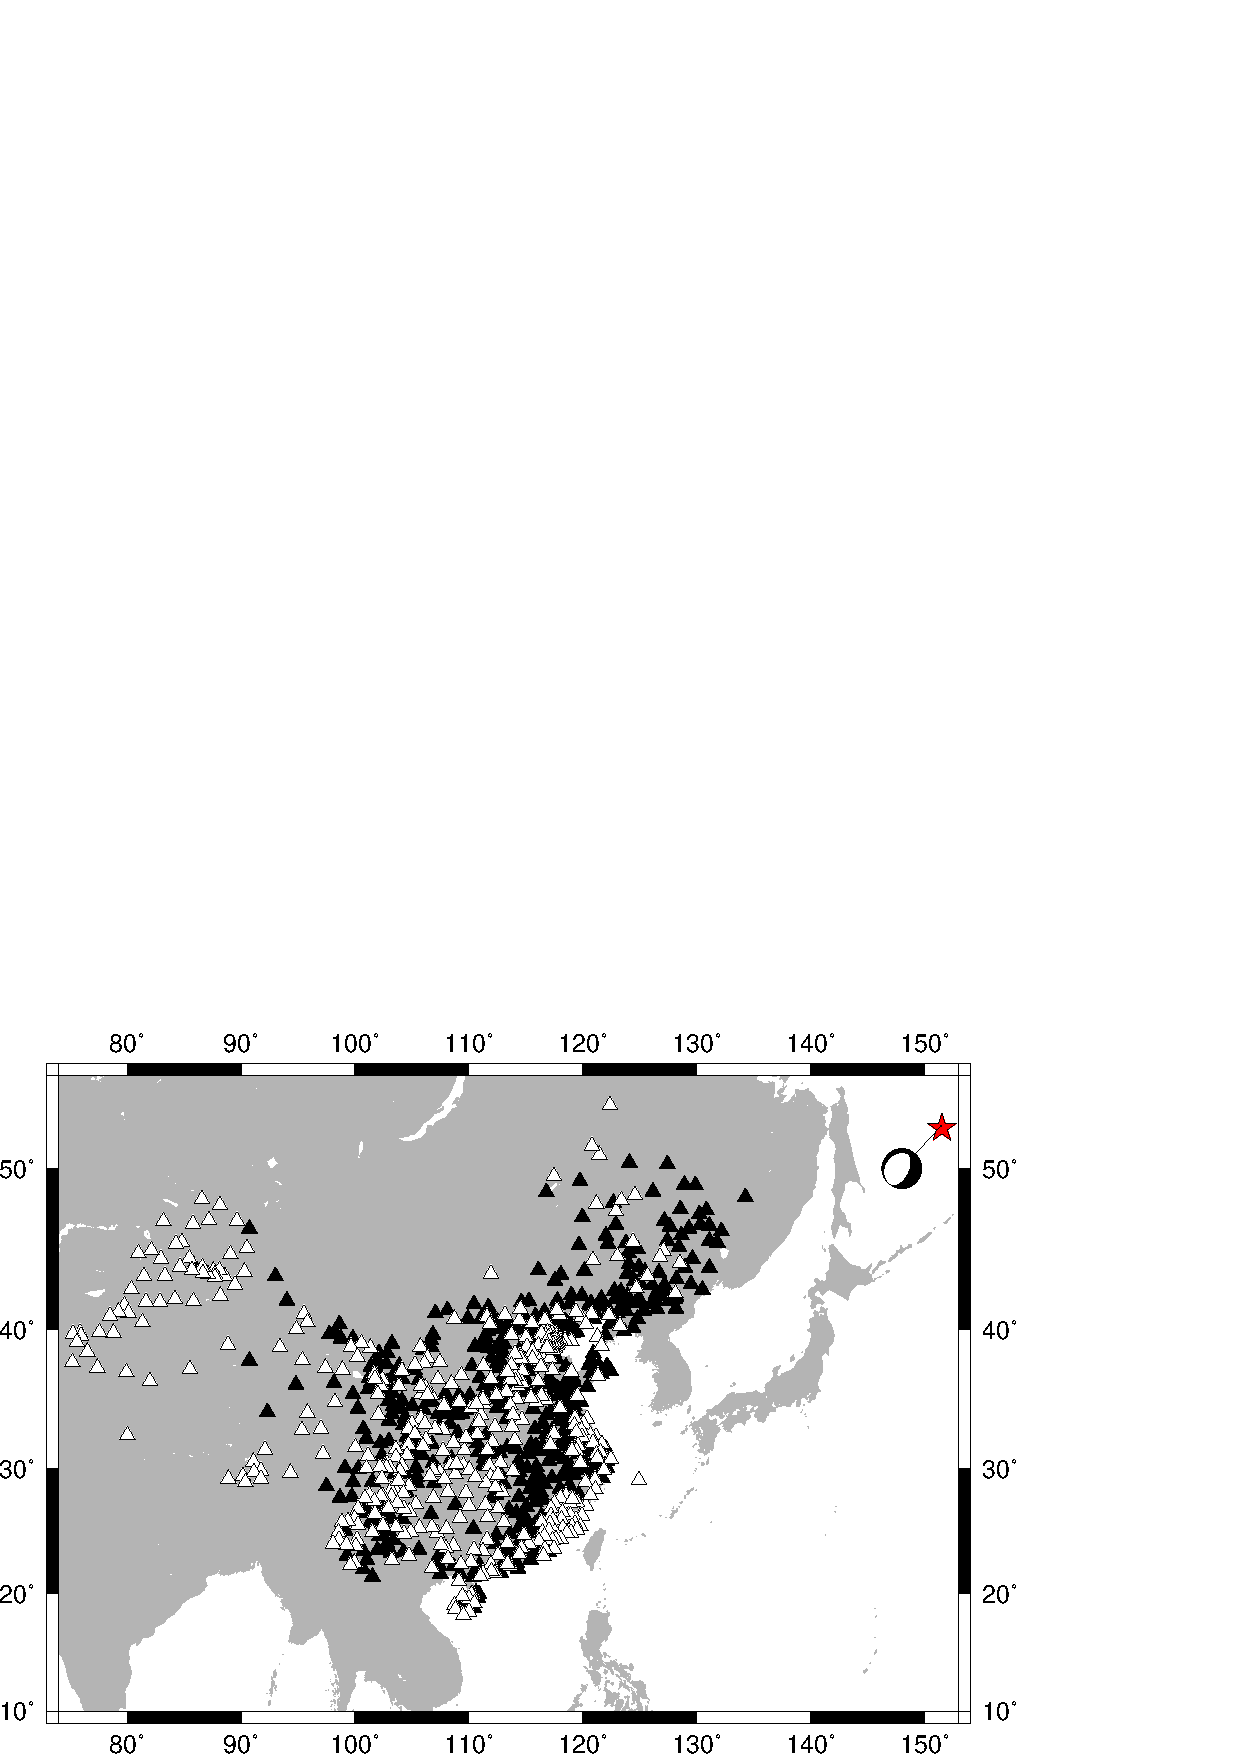
\includegraphics[width=0.8\linewidth]{fig/chap2/ev_sta_2013}
\caption{图\ref{cn_2013}中记录对应的台阵分布和地震位置. 黑色三角形表示记录到PKiKP信号的台站,白色的表示未记录到PKiKP信号的台站.}
\label{fig:ev_sta_2013}
\end{figure}

由于缺少东亚的IMS台站数据,这里用日本Hi-net台网和国家测震台网对东亚下方的CMB/ICB进行补充采样. 由于这些密集台网的台站数量均超过700个,所以不便用来搜索PKiKP观测. 于是本研究采用先用单个稳定的固定台先对附近的地震事件进行搜索,找到能产生PKiKP的事件,这里使用牡丹江台(MDJ)进行搜索近二十年的地震事件. 使用这种方法,利用国家测震台网观测到两个产生500个以上清晰PKiKP信号的地震事件,这在世界上也是首次得到如此连续的跨度达到40{\textdegree}震中距的记录(图\ref{cn_2011}和图\ref{cn_2013}). 尤其值得注意的是图\ref{cn_2011}中云南台网记录到的小于4{\textdegree}的清晰PKiKP波形,如此小震中距下仍然有清晰的内核反射震相,暗示了尖锐ICB的存在. 要产生大量的PKiKP反射必然要满足很多条件,首先必须要有足够大的震级激发出足够强的PKiKP信号,这两个地震均超过6级,相比而言,由牡丹江台搜索出的其他较小震级地震就没能产生类似的PKiKP观测数量;其次,地震需要有合适的震源辐射花样,PKiKP的离源角应该指向辐射能量大的方向,通过Harvd全球CMT解(\url{http://www.globalcmt.org/})计算,这也得到了验证(图\ref{fig:rad});除了震源因素,台阵场地效应、台阵周围的噪声环境都能影响PKiKP的观测. 就以上两个地震而言,中国中部普遍缺少PKiKP观测(图\ref{fig:ev_sta_2011},\ref{fig:ev_sta_2013}),正是源于台站下方的沉积层对PKiKP能量的衰减作用,而位于山地的台站,由于其台基在基岩之上,普遍都有清晰的PKiKP记录.


 

\begin{figure}[ht]
\centering
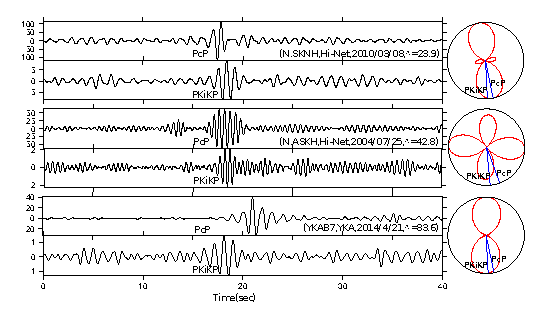
\includegraphics[width=0.8\linewidth]{fig/chap2/rad}
\caption{Hi-net和YKA台站记录到的三个不同震中距地震事件产生的PcP、PKiKP波形(左),和对应的P波辐射花样(右). 在小震中距情况下两者的离源角相差不大(上、下),当震中距增大时PcP和PKiKP的辐射能量有明显差异(中). }
\label{fig:rad}
\end{figure}


\section{数据处理方法}

这一节介绍研究中的数据处理方法. 包括搜索PKiKP信号用到的叠加方法,计算台阵平均PKiKP/PcP振幅比和平均差异走时残差的方法以及数据筛选的一些准则. 

\subsection{PKiKP信号的预识别}

如前文所提到,本研究需要从全球的IMS台阵数据中挑选可识别的PKiKP信号,但是人工挑选由于可能存在的肉眼识别偏差,会遗漏某些产生PKiKP信号的地震事件,虽然单个台站记录不太明显,但叠加后的波形却十分清晰. 本文所使用的均是能产生清晰叠加结果的记录,叠加方法使用的是PWS. 

PWS方法最早见于地幔间断面转换波的探测~\citep{Schimmel1997},能够增强连续的一致信号,压制不连续的随机噪声,目前较为广泛地用于弱信号的识别. 典型的例子就有其应用于前临界PKiKP的研究
~\citep{Koper2003,Koper2004},还有用于寻找穿过内核的S波震相PKJKP~\citep{Deuss2000}以及识别在内核内侧反射的PKIIKP震相~\citep{Niu2008}. 下面将简要介绍PWS方法的原理和其叠加效果. 

PWS是一种非线性叠加方法,它使用一种不依赖振幅的一致性度量方法来加权线性叠加. 在叠加的过程中
首先要构建一个解析复信号$S(t)$,它的实部是台站接收到的信号$s(t)$,虚部是则是实部的希尔伯特
变换

\begin{equation}
S(t) = s(t) + i \mathscr{H} [s(t)]
\end{equation}

上式可以写成振幅和震相分离的形式

\begin{equation}
S(t) = A(t) exp[i \Phi (t)]
\end{equation}

其中$A(t)$是地震信号的波包,$\Phi (t)$为瞬时震相. 震相叠加的表达式如下

\begin{equation}
c(t) = \frac{1}{N} \left| \sum_{j=1}^{N} exp[i \Phi_j (t)] \right|
\end{equation}

用震相的$\nu$次幂作为加权系数,就得到了PWS的表达式

\begin{equation}
 \nu_{PWS}(t) = \frac{1}{N} \sum_{j=1}^{N} s_j (t)c^{\nu} (t)
\end{equation}

当加权系数取0的时候即为常规的线性叠加,本研究中PWS加权系数均取2. 除此之外,在预挑选过程中不做慢度偏移,直接进行零慢度叠加. 首先,这样给数据处理带来了方便;其次,IMS台阵的口径都很小,对慢度的分辨能力很低~\citep{Rost2002},零慢度叠加常常就能得到很好的效果. 图\ref{fig:stack}分别对比了YKA台阵中对某个地震事件的单台记录、线性叠加和PWS叠加结果. 可以明显看出,叠加之后的微弱PKiKP信号明显增强. 这里需要特别提到,这里的叠加仅仅是为了对地震事件进行挑选,由于叠加之后的的振幅并不能体现出真实的振幅信息,因此不参与后面的振幅比计算. 

\begin{figure}
\centering
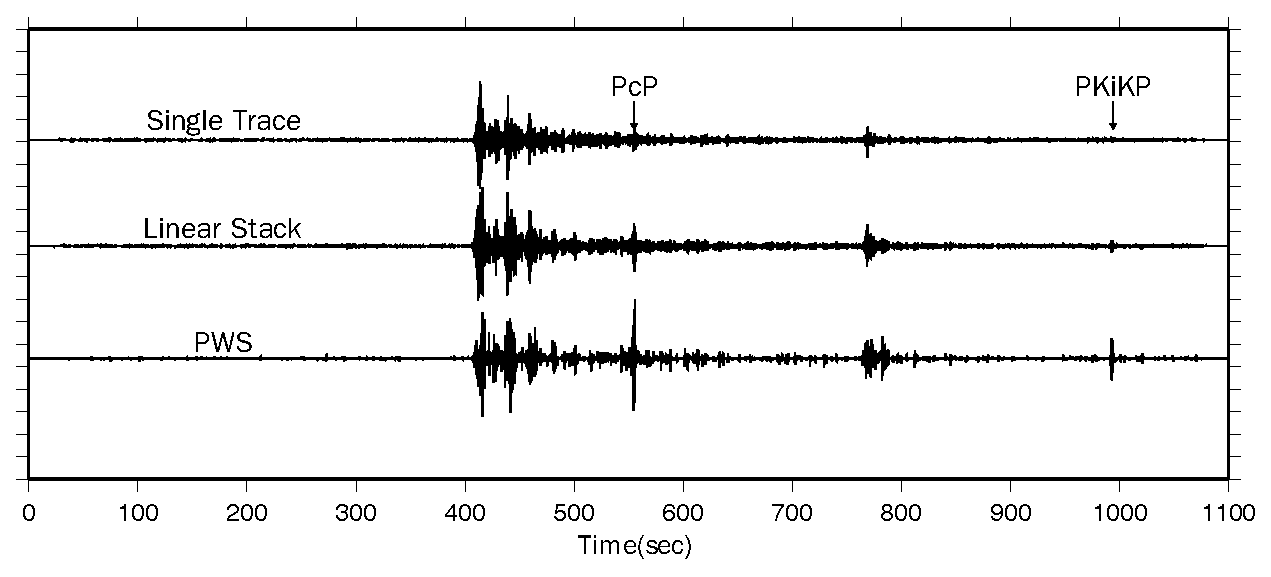
\includegraphics[width=0.8\linewidth]{fig/chap2/stack}
\caption{YKA台阵对事件2014/06/03,22:29:51(106 km, Mb6.0)的单道记录和叠加结果比较. 图中上为台阵中某单道记录,中间为线性叠加结果,下为PWS处理后的结果. }
\label{fig:stack}
\end{figure}

\subsection{振幅比和走时残差的计算}

\subsubsection{PKiKP/PcP振幅比}

前人利用IMS台阵数据研究内核边界通常使用的是所有台站记录经过线性叠加后得到叠加记录的PKiKP/PcP振幅比,最终每一个事件-台阵对就仅只剩下一个振幅比数据~\citep{Koper2004a}. 这样做虽然得到了一个平均的比值,但却丢失了很多信息. 因为即使是口径仅20千米的小口径台阵,每个台阵的记录差别可能依然会很大,而且尤其
体现在PcP的振幅差别上,因为PcP比PKiKP更容易受到浅层结构的影响. 产生差别的原因有很多,其中一个比较重要的
就是每个台站下方的物性差异. 比如,台站下方介质比较致密的岩石的台站记录到的PcP振幅就会比下方是松软沉积
层的台站记录到要大. 如果仅仅做简单的叠加,得到的振幅比可能与真实值相差很大,同时也不能得到振幅比测量
值的可信度估计. 

考虑到台阵内存在的不确定性,本研究采用计算台阵平均振幅比的方法,即先计算台阵内每个台站的PKiKP/PcP振幅比然后再计算所有台站的平均值. 假设台阵内的台站数为$N$,第$i$个台记录的PcP和PKiKP振幅分别为$A_i^{PcP}$和$A_i^{PKiKP}$,则该台的振幅比为

\begin{equation}
r_i = \frac{A_i^{PKiKP}}{A_i^{PcP}}
\end{equation}

于是可以得到台阵的平均振幅比

\begin{equation}
\overline{r} = \frac{1}{N} \sum_{i=1}^{N} r_i
\end{equation}

还可计算每个台阵振幅比的标准差,用于振幅比测量的可靠性评价

\begin{equation}
\sigma = \sqrt{\frac{\sum_{i=1}^{N} (r_i - \overline{r} )}{N}}
\end{equation}

虽然采用台阵平均振幅比有其优越性,但有的时候测量每个台阵的振幅比却会遇到困难,因为当信噪比过低的时候相
位的振幅不容易读出来. 因此关于每道记录的PKiKP/PcP振幅测量,采用如下方法:首先根据预叠加结果找到震相
最大振幅的位置,然后在所有台站记录中找到质量最好震相的最大振幅峰值位置,再对其他各道记录注意追踪震相,
以其峰值作为振幅,如果不能追踪,则剔除该道记录. 当然,对于每道记录,这个峰值并不一定是该信号的最大振幅
值,但即使这样也并不会有太大差异,而且这些差异都最终体现在平均振幅比的标准差上. 

前面提到在震中距较大时PcP和PKiKP离源角有比较大的差异,因此需要做震源辐射校正,否则可能对后续的振幅比分析产生影响. 根据~\citep{Aki2002a},远场P波辐射花样可以表示为,

\begin{equation}
\mathcal{F}^P = \bm{\gamma} \cdot \bm{M} \cdot \bm{\gamma}
\end{equation}

其中$\bm{M}$是矩张量,而$\bm{\gamma}$为P波极化方向,可以用离源角$i_{\xi}$和方位角$\phi$表示

\begin{equation}
\bm{\gamma} = \left(\begin{array}{c}
\sin i_{\xi} \cos \phi \\
\sin i_{\xi} \sin \phi \\
\cos i_{\xi}
\end{array}\right)
\end{equation}

做震源辐射校正即将关测的振幅比乘上PcP和PKiKP辐射因子的比值%
$\frac{\mathcal{F}^{PcP}}{\mathcal{F}^{PKiKP}}$. 

\subsubsection{PKiKP-PcP走时残差}

对于PKiKP-PcP走时残差,其计算方法和台阵平均振幅比类似,也是先得到每一个台站的走时残差,再计算整个台
阵的平均值. 本研究中,PcP和PKiKP的走时差均认为是其峰峰或者谷谷的时差;残差则是相对于PREM而言,这是
因为在该模型的构建过程中加入了PcP-PKiKP走时观测结果,使得其与实际观测资料能有比较好的拟合度. 影响PK
iKP-PcP走时残差的影响因素除了相对PREM的局部的内外核厚度变化,还有地球的椭率和两个震相经过的地幔部分
速度的差异. 但在本研究中不考虑后两种因素,首先本研究分析所用的IMS台阵数据采样的CMB区域非常小,因此假
定这两个因素对残差的贡献很小. 而且分析考虑的是走时残差的相对变化,并由此推测CMB的小尺度结构,所以走时
残差仅做如下计算,

\begin{equation} T_{res} = (T_{PKiKP}^{obs} - T_{PcP}^{obs}) - (T_{PKiKP}^{prem} - T_{PcP}^{prem})
\end{equation}

相比与台阵平均振幅比的不确定性, 每个台站的相对走时残差的差异都很小,平均走时残差的标准差一般为0.01秒的量级,这也体现出走时观测比振幅观测要稳定可靠得多. 

\chapter{IMS台阵数据约束CMB结构变化}

利用PKiKP和PcP的振幅比可以约束ICB的密度和波速变化~\citep{Koper2004a},即认为在小震中距情况下,PcP和PKiKP在地幔中的传播路径比较接近,则地幔对振幅观测的影响可以基本消除,同时也可以避免由于仪器增益
差异造成的绝对振幅不准确的影响,振幅比异常的贡献主要来自于内核,从而可以据此估计内外核边界的物理参数
. 但利用振幅比研究ICB结构有几个重要的假设,即核幔边界起伏很小,且PKiKP/PcP振幅比对核幔边界的物
性参数变化不敏感. 引言中已经提到,一些研究已经揭示出CMB可能存在小尺度的起伏~\citep{Rost2004a},且对PcP会造成显著的聚焦或发散效应,引起其振幅出现较大变化~\citep{Wu2014a,Shen2016};存在于CMB及其上方的低速异常结构~\citep{He2009}也会降低反射PcP的振幅. 在受到这些影响的情况下,利用PKiKP/PcP振幅比来估计ICB的物性参数就会很困难;若CMB存在厚的转换带~\citep{Garnero2000},且转换带的厚度接近与入射PcP的波长,其反射系数也会剧烈减小~\citep{Richards1972}. 

通过分析所收集的PKiKP和PcP数据,本研究发现CMB小尺度变化的确是造成振幅比变化的重要因素. 首先,在所有
观测到PKiKP的300个事件-台阵对数据中,仅有不到一半的数据中同时出现可观测的PcP和PKiKP信号. 影响这
两个震相同时可观测性的因素有很多,主要包括(1) 震源的参数,即震源深度和震级. 震源深度增大会同时增大PcP和PKiKP离源角的差异,而震级太小的地震则不足以产生足够强的反射能量;(2) 震中距. 由于不同震中距对应不同的PcP和PKiKP的入射角,且由图\ref{fig:rtf}可知,不同入射角下的PcP和PKiKP反射系数可能会有比较大的不同;(3) CMB、ICB及它们顶部的结构. PcP和PKiKP均为由不连续界面反射的震相,因此,它们的振幅对反射界面的性质和结构变化非常敏感. 为了初步确定影响PcP可观测性的因素,这里对所有IMS台阵数据的分布做了一些统计分析,即PcP可观测性随震源深度、地震震级(图\ref{dep_mag_hist})和震中距(图\ref{dis_hist})的分布. 从结果来看,对于本研究收集的IMS数据而言,不管是地震的震级、震源深度还是还是震中距都不会
对这两个震相是否能被同时观测到产生太大的影响. Mw5.0震级之上的事件都能够产生可观测的PcP和PKiKP信
号,这些地震深度也基本集中在0--100km,这说明在最初对事件的选择上不加太多限制是正确的,较多的5级地震
保证了有效数据的数量. 

由于震源深度并不对PKiKP和PcP的同时可观测性产生很大影响,因此可以很大程度上排除未能观测到PcP但观测到
PKiKP是上地幔结构的影响,比如俯冲板块对PcP的振幅的衰减作用. 这就更加强烈暗示了核幔边界的结构是影响P
cP观测的主要因素,也隐含了CMB结构对PKiKP/PcP振幅比可能产生巨大影响. 从观测到和未观测到的PcP在CMB
的反射点分布来看,即使在某个较小的区域内,PcP的观测性都会存在交替变化(图\ref{loc_distri}). 如前
面提到,CMB对PcP的影响因素也并非单一,仅考虑某一因素也常常不能解释为理论预期数倍的振幅比观测~\citep{Koper2004a},本章则尝试结合前人的观测和理论模拟结果,并对IMS台阵-事件对数据进行对比分析,尝试确定造成PKiKP/PcP振幅比和走时观测异常的CMB结构,包括CMB的小尺度起伏和低速异常结构. 

\begin{figure}
	\centering
	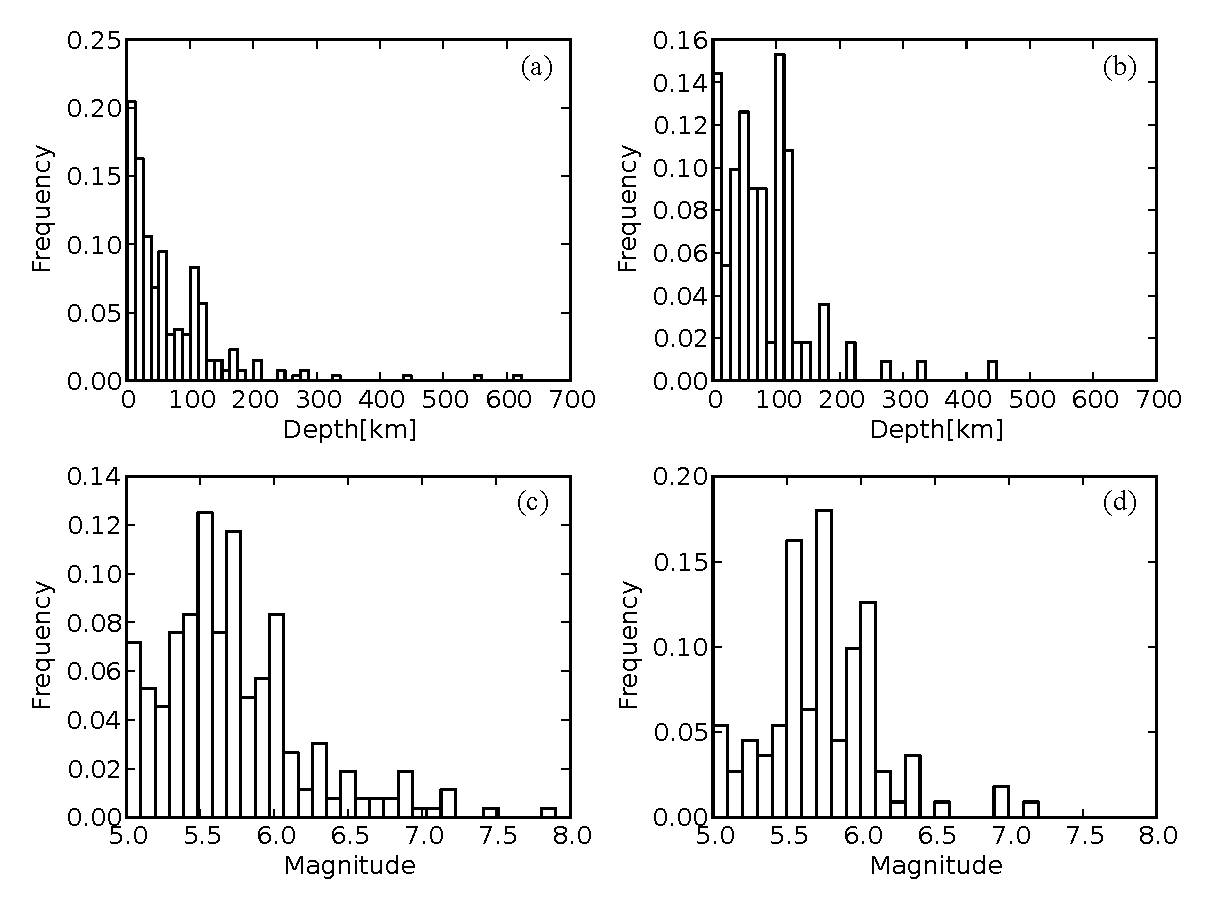
\includegraphics[width=0.85\linewidth]{fig/chap4/depmag_hist1.eps}
	\caption{(a)、(b)分别为观测到PKiKP震相的事件和同时观测到PcP和PKiKP的事件随震源深度%
的分布;(c)、(d)分别为观测到PKiKP震相的事件和同时观测到PcP和PKiKP的事件随震级的分布. }
	\label{dep_mag_hist}
\end{figure}

\begin{figure}
	\centering
	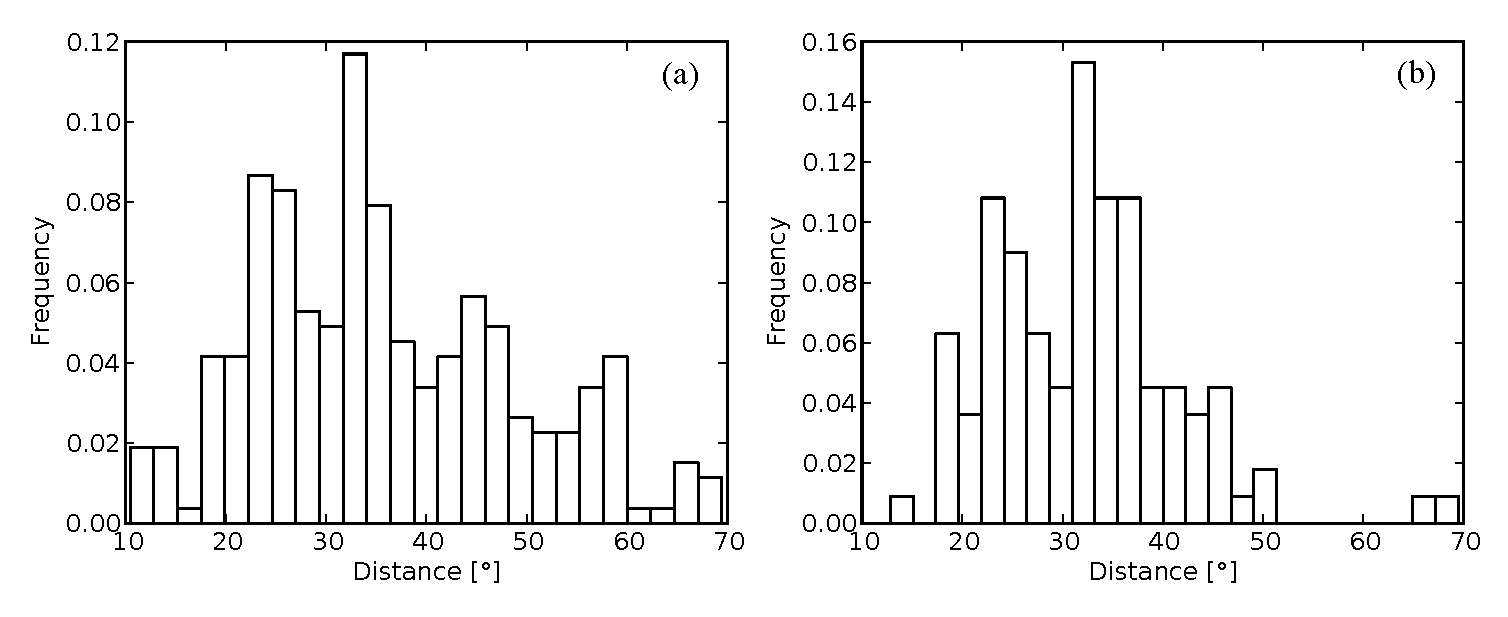
\includegraphics[width=0.85\linewidth]{fig/chap4/dist_hist1.eps}
	\caption{(a)、(b)分别为观测到PKiKP震相的事件和同时观测到PcP和PKiKP的事件随震中距%
的分布. }
	\label{dis_hist}
\end{figure}

\begin{figure}
	\centering
	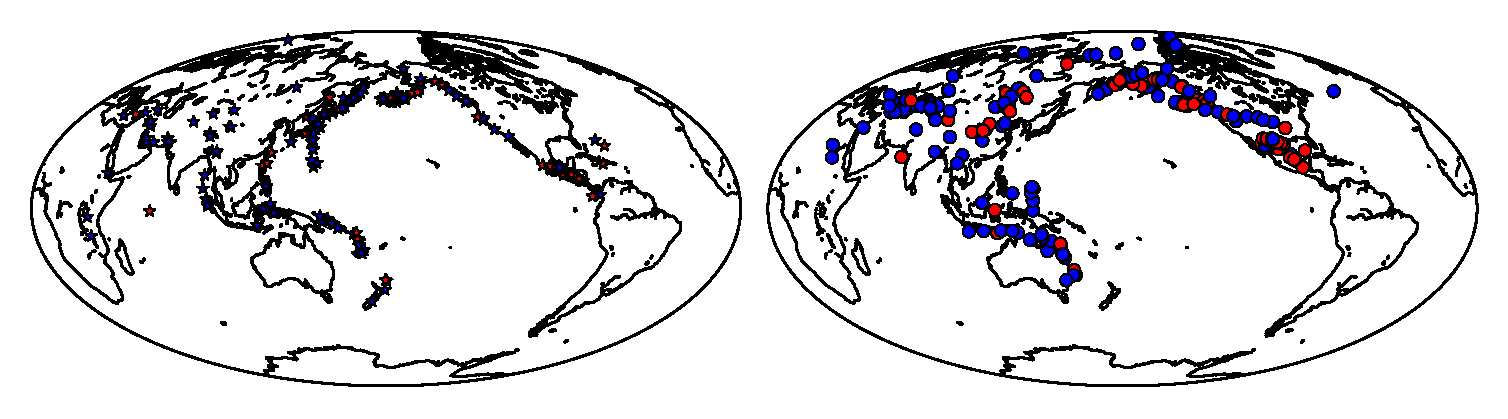
\includegraphics[width=\linewidth]{fig/chap4/loc_distri.eps}
	\caption{左图为地震事件的分布,红色五角星表示同时观测到PKiKP和PcP的事件,蓝色五角星表示%
仅观测到PKiKP的事件;右图为PcP在CMB的上的反射点分布,红色圆圈表示同时观测到PKiKP和PcP,蓝色%
圆圈表示仅观测到PKiKP的反射点. 红色与蓝色的交替体暗示CMB存在小尺度结构的变化. }
	\label{loc_distri}
\end{figure}

\section{CMB界面起伏}

CMB的界面起伏包括其上凸和下陷,分别会造成PcP的发散和汇聚,从而减小或增大台站记录到的PcP振幅~\citep{Neuberg1991}. 本小结基于采样相邻CMB和ICB区域的PKiKP与PcP的振幅比的差异,并结合相对PREM的差异走时残差分析CMB的小尺度起伏变化. 由于本研究主要考虑确定对PcP产生影响的CMB变化因素,因此重点关注的是相邻采样点的振幅比和走时残差的差异,并不要求根据绝对值来约束CMB变化的细节,因此不对所有的观测数据作过多解释. 

\subsection{CMB的局部上凸}

 前人利用全球PKiKP和PcP数据研究ICB物性参数的研究都曾报道过某些区域存在较大的振幅比值,例如\citet{Koper2004a}观测到Vanuatu俯冲带的地震产生的接近理论PREM预测十倍的观测振幅比,并将其解释为CMB起伏和波速异常的综合效应;\citet{Waszek2015a}则将很多大的振幅比观测归结于ICB对PKiKP的放大. 本研究
中采样中美洲下方的CMB的NVAR和PDAR数据很大程度上可以用一个局部上凸的CMB来解释. 对于表\ref{evt}
中前10个地震事件,它们产生的PcP和PKiKP同时被NVAR与PDAR记录到,本研究通过比较与CMB上不同的PcP反
射点位置所对应的PKiKP/PcP振幅比,发现了对于不同反射区域,振幅比存在非常明显的差异. 这10个地震按照地
理位置关系大致可以被划分为两组. 纬度较高的一组包含3个地震,位于墨西哥南部;而纬度较低的一组包含7个地
震,位于危地马拉地震带(图\ref{map}a). 位于下方的一组中的地震的震源机制相似正断型的震源机制,但深
度都不相同,从数十至一百km左右. 

\begin{figure}
\centering
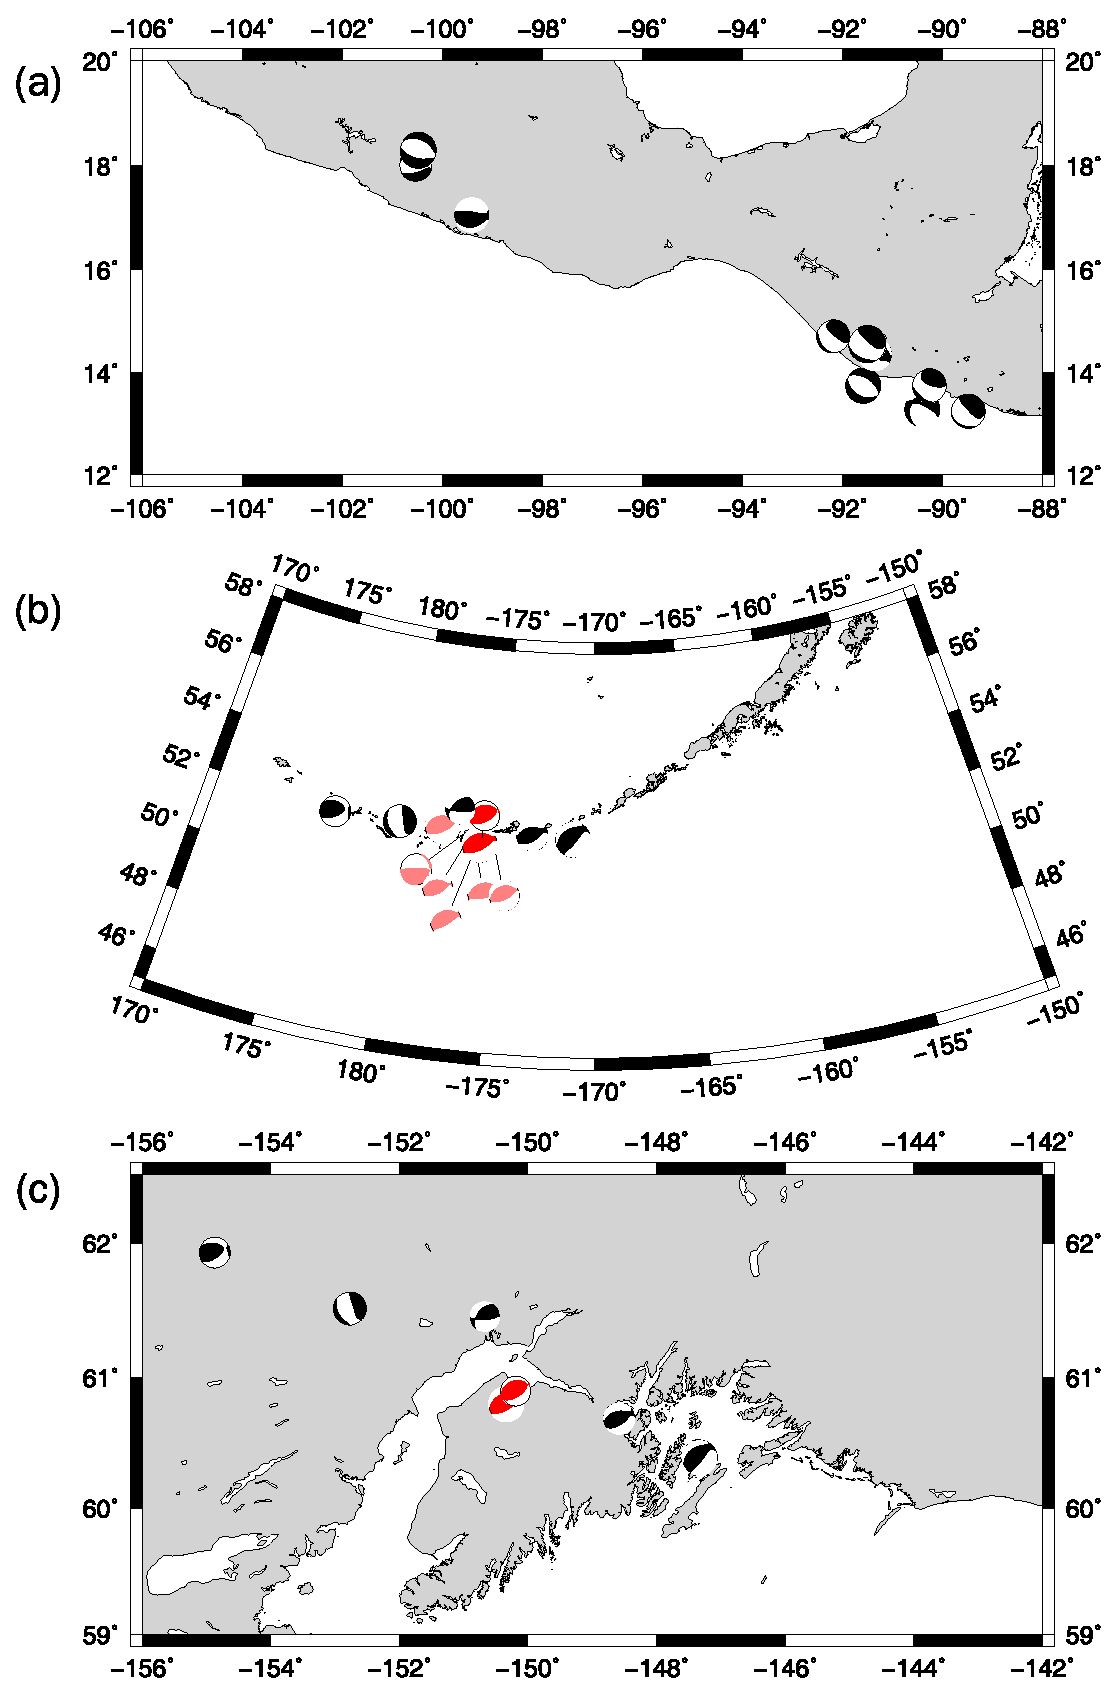
\includegraphics[width=0.7\linewidth]{fig/chap3/evt_bp.eps}
\caption{(a)~表\ref{evt}中第1--10号地震的位置;(b)~黑色和红色的震源球表示是表\ref{evt}中第11--17号地震, 红色震源球表示产生相对与相邻地震异常小的振幅比的事件. 浅红色的震源球表示地震产生与小振幅比事件相似的大振幅PcP,但没有PKiKP的观测;(c)~(b)中黑色和红色事件产生的PcP在CMB上的反射点位置. }
\label{map}
\end{figure}

根据这十个地震-台阵对的PcP反射点的位置,可以在CMB上划分出四个小反射区域,如图\ref{ratio_loc}所
示. 通过测量每个事件-台阵平均PKiKP/PcP振幅比,可以注意到对应于位于危地马拉的7个地震,NVAR和PDAR
记录到的振幅比的明显差异(图\ref{ratio_loc}b),这也体现出相应的CMB上的PcP反射区域1和4的性质存
在明显的差异. 对于NVAR,其观测振幅比相比于由PDAR记录的振幅比要小很多,然而这两个台阵的震中距比较接近,仅相差1{\textdegree}左右,因此可以排除震中距差异的影响. 对于下方7个地震的振幅比测量,NVAR的结果
几乎都是0.03左右,且平均振幅比的标准差全小于0.008,仅有事件7稍大为0.067,与PREM对各项同性源的预测
值0.04还是比较接近的. 这也体现出对于这些地震,NVAR的振幅比测量结果是比较稳定和可信的. 与NVAR台阵的测
量结果相反,使用PDAR的记录得到的PKiKP/PcP振幅比则普遍偏大,均为PREM理论值的两倍以上,同时也具有很
大的标准差. 关于标准差的差异,可以解释为,当PcP振幅很大且变化不大的情况下,由于其位于分母且PKiKP振幅
都比较小,造成最终的振幅比偏小且每道的值相差不大,这就对应NVAR的结果;而PcP振幅较小,若其稍有变化,
便使得振幅比有较大的变化,这就对应PDAR的情况. 以上分析也表明,PDAR记录到的PcP受到了强烈的衰减. 对于
上方3个地震,NVAR和PDAR的观测振幅还较为接近,均为PREM预测的数倍. 

进一步比较采样区域1和4的数据,可以推断出CMB结构对振幅比的强烈变化有重要贡献. 首先,从振幅的角度看,与
相对稳定PKiKP相比,两个位置反射的PcP振幅显示出了很大的差异. 对于事件10,在观测的频率范围(1--2 Hz) ,NVAR和PDAR记录的PcP振幅大小明显不同,NVAR的PcP叠加振幅要比PDAR的要大6倍以上,然而,两个台阵的叠加PKiKP振幅却十分相近(图\ref{amp_nv_pd});其次,从波形的角度来看,采样两个区域的PcP波形也存在显著差异(图\ref{amp_nv_pd},\ref{pcp_pkikp_nvpd}). 采样区域1的PcP波形显得相对尖锐,而采样区域4的PcP显得波形被延长了;与PcP的差异产生鲜明对比的是,两个台阵记录的PKiKP波形都显得清晰尖锐. 除此之外,由NVAR记录的PcP波形与两台阵记录的PKiKP波形也比较相似. 不仅对事件10,出现这种现象,对于图\ref{map}中下方其他几个地震也是如此. 这就有力地表明,造成PcP波形和振幅的变化的源头并非来自浅部的衰减或不均匀结构,因为在浅部PKiKP和PcP具有相近的传播路径,因而会有相似的特点. 所以可以把造成PcP和PKiKP/PcP振幅比差异的源头继续追踪至CMB的结构. NVAR和PDAR间距约为1000km,而1和4两个反射区域在CMB上距离约为280km,这可能暗示了CMB在中等尺度下的变化. 

\begin{figure}
\centering
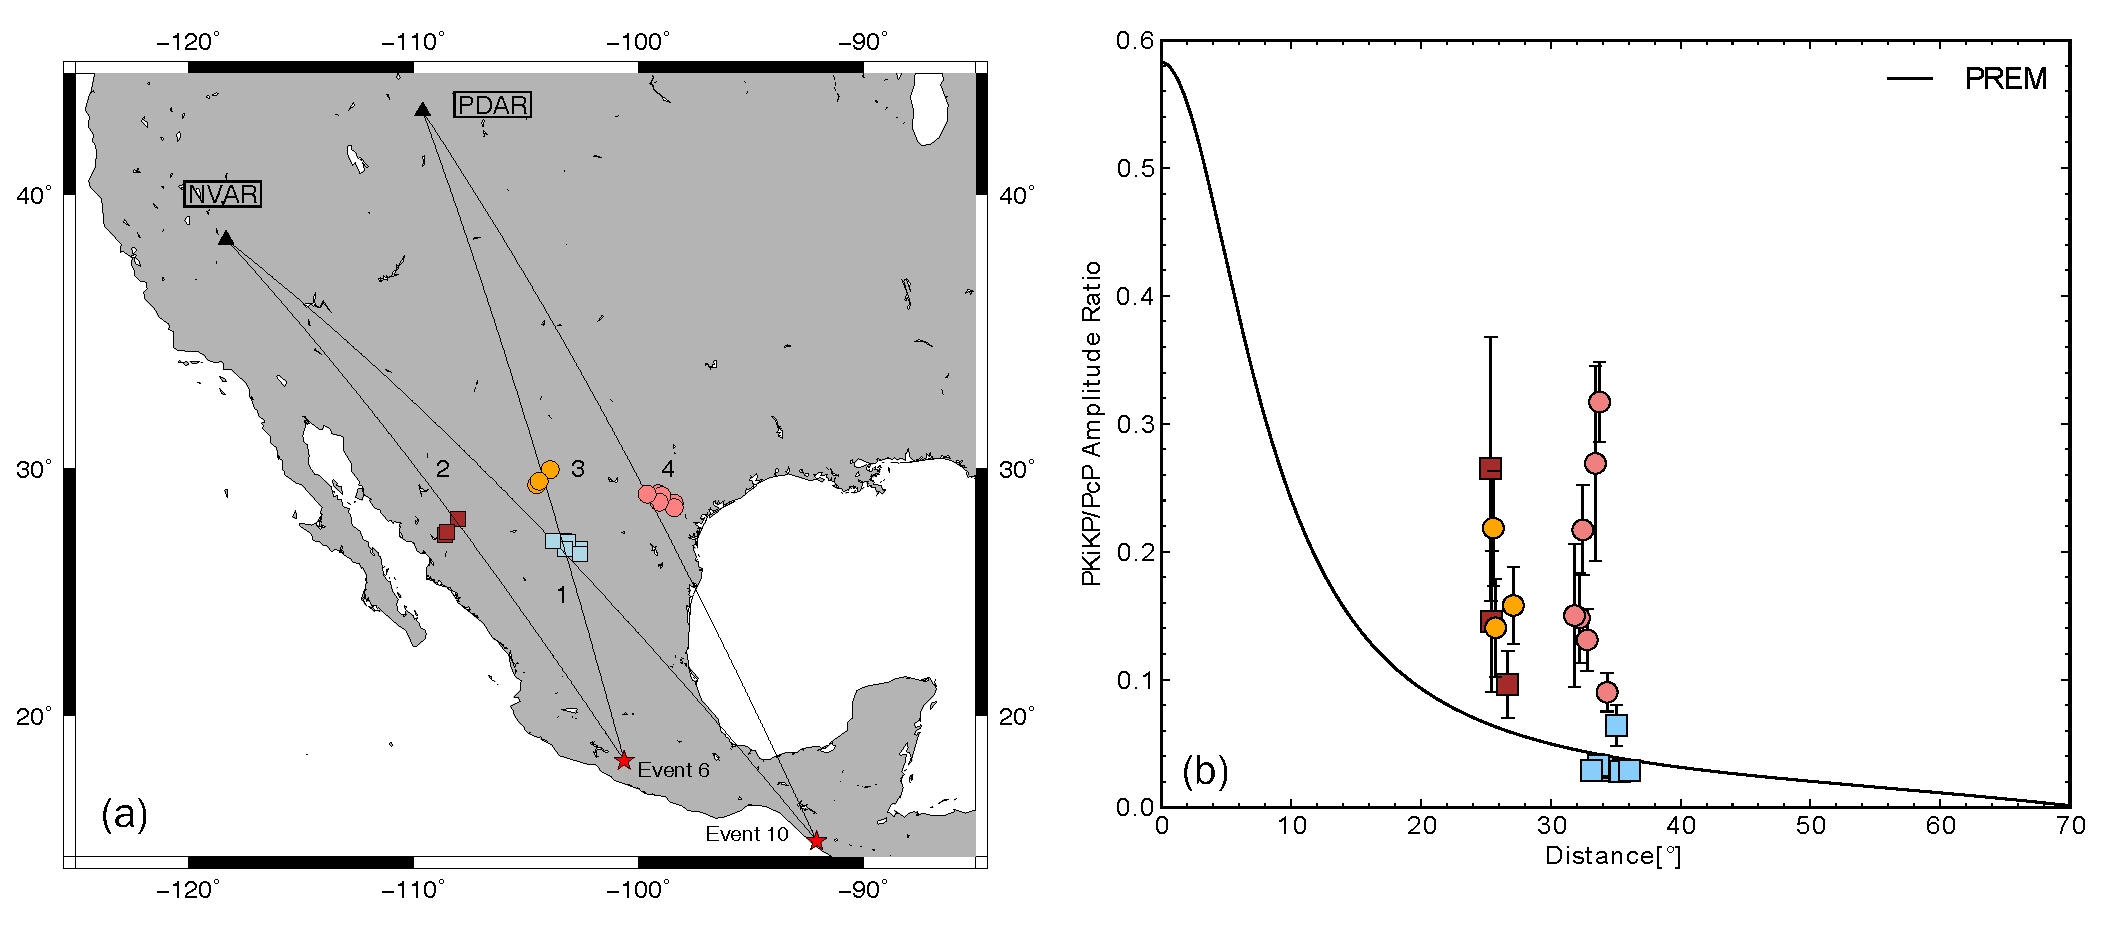
\includegraphics[width=\linewidth]{fig/chap3/evt_bp_us.eps}
\caption{(a)~台阵NVAR、PDAR和表\ref{evt}中前十个事件的PcP反射点位置. 两个台阵和事件6、10的位置也被画出. 浅蓝色圆圈表示相应与较低PKiKP/PcP振幅比的PcP反射点位置,浅红色圆圈则表示相对大的振幅比. 四个PcP反射区域用数字1--4标出;(b)~NVAR和PDAR观测到的由图\ref{map}下方事件组产生的PKiKP与PcP信号的振幅比. 可以看出两个台阵观测的明显差异. PREM对与一个各项同性源的预测振幅比值也被画出,作为参考. }
\label{ratio_loc}
\end{figure}

\begin{figure}
\centering
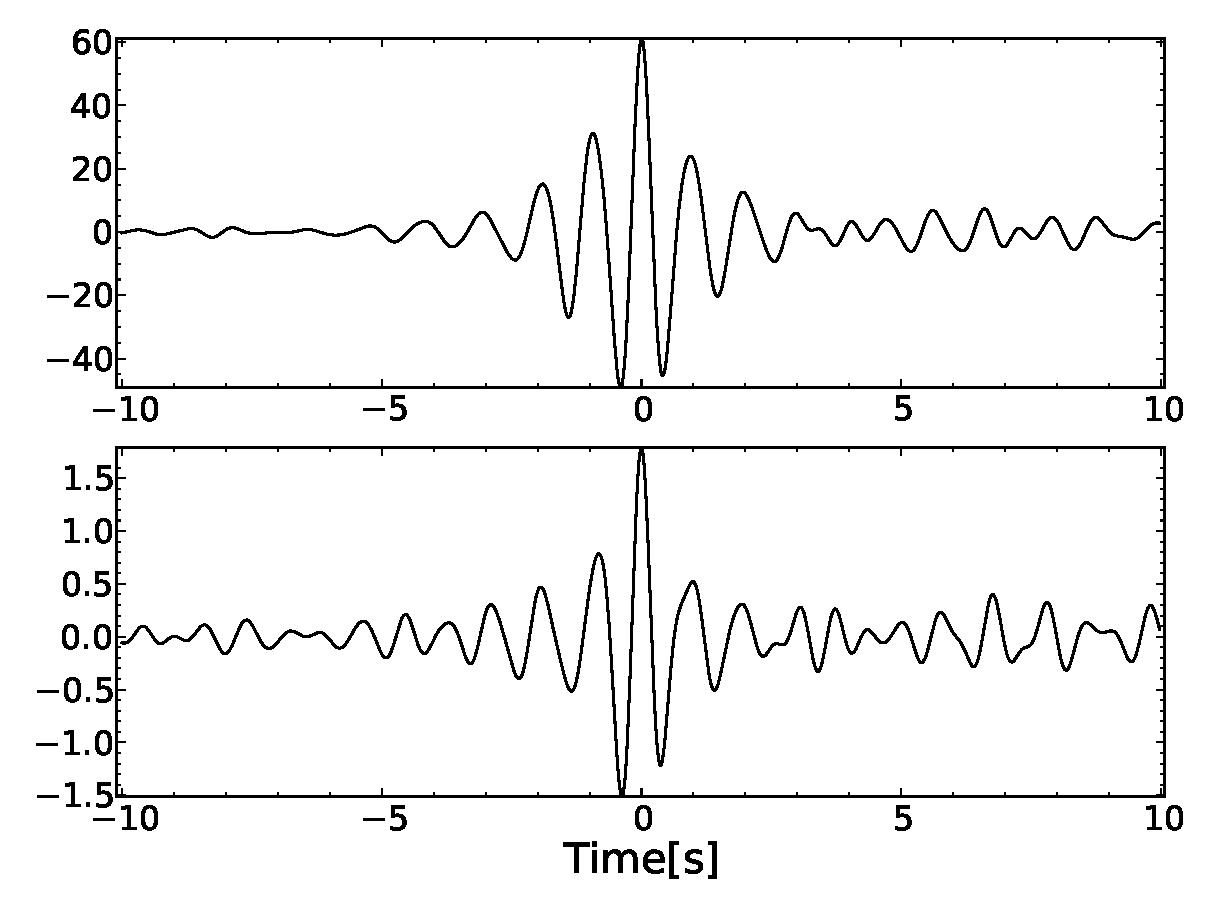
\includegraphics[width=0.4\linewidth]{fig/chap3/amp_nv_4371355_s.eps}
\quad
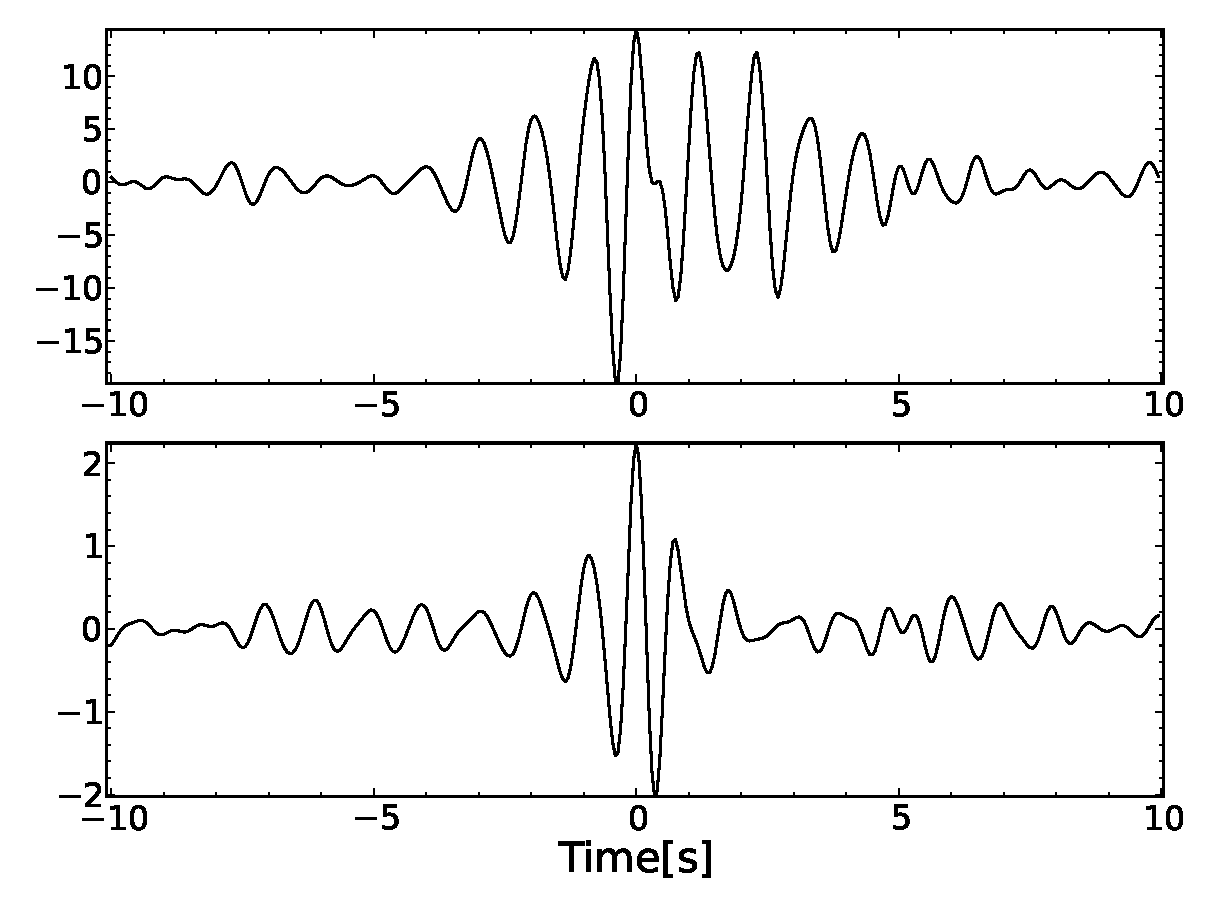
\includegraphics[width=0.4\linewidth]{fig/chap3/amp_pd_4371355_s.eps}
\caption{表\ref{evt}中事件10产生的PcP and PKiKP,分别由(a)~NVAR和(b)~PDAR所记录. 波形均为台阵内所有台站的叠加,震中距标在图的左上角. }
\label{amp_nv_pd}
\end{figure}

\begin{figure}
\centering
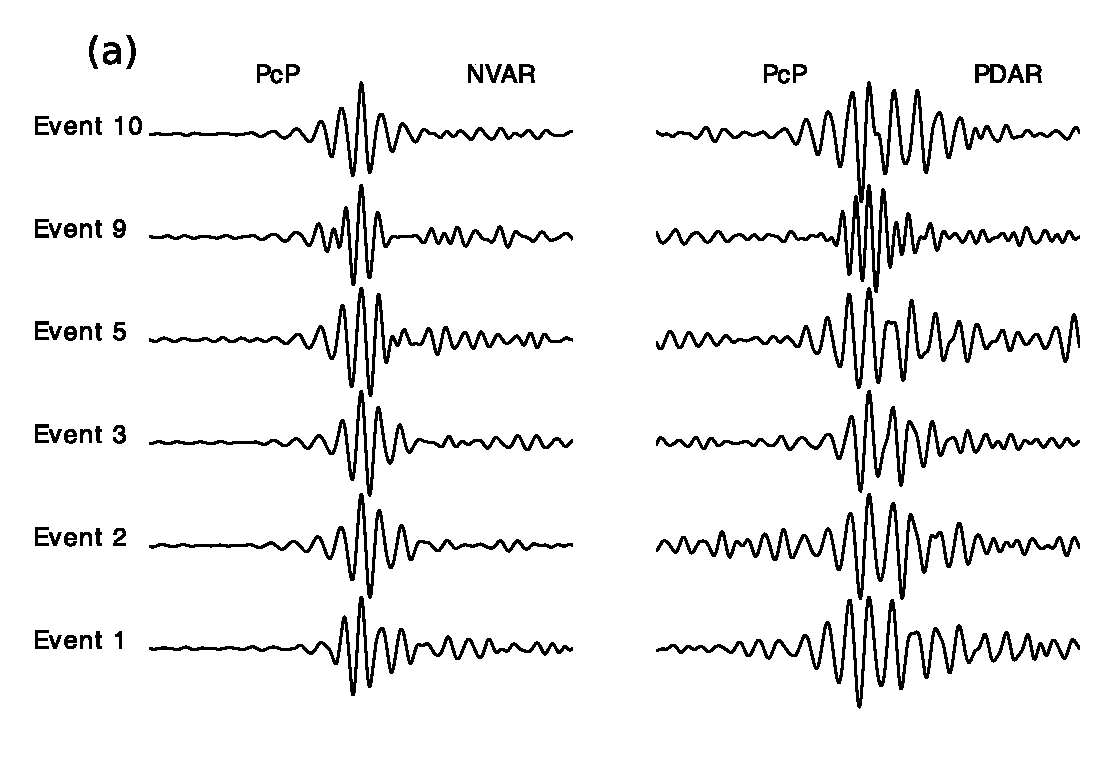
\includegraphics[width=0.7\linewidth]{fig/chap3/pcp_nvpd.eps}
\\
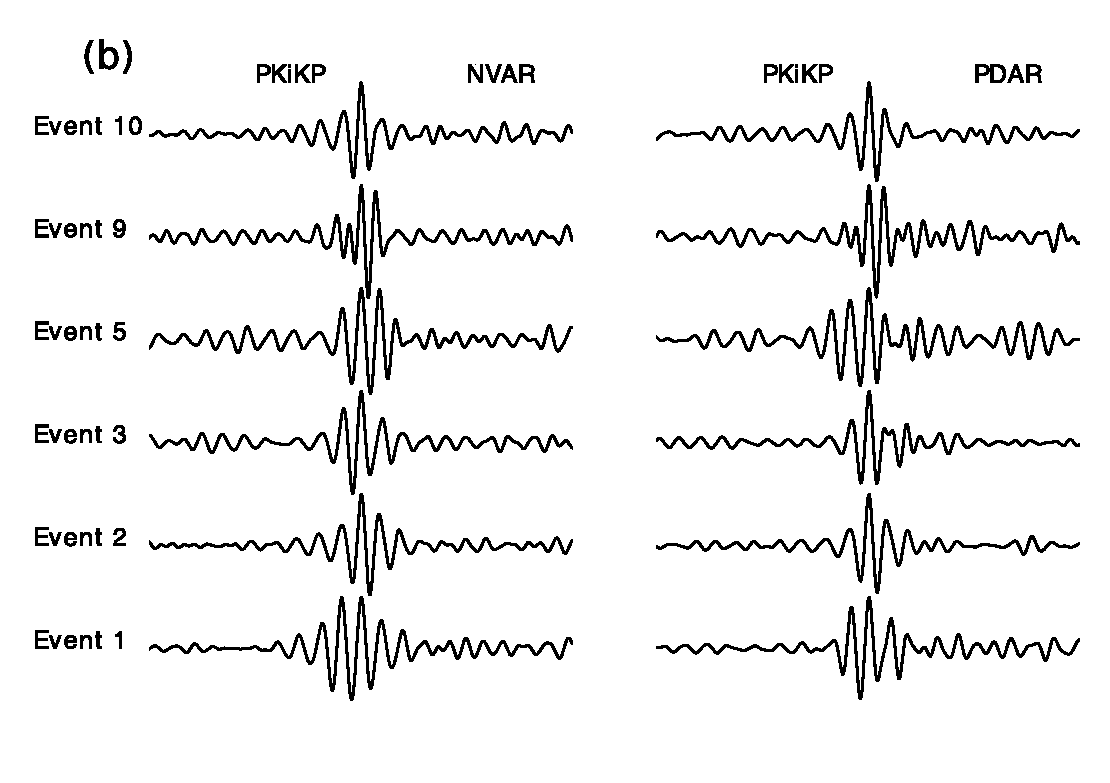
\includegraphics[width=0.7\linewidth]{fig/chap3/pkikp_nvpd.eps}
\caption{NVAR和PDAR记录的表\ref{evt}中6个事件的PcP(a)和PKiKP(b)波形比较. 采样区域1和区域4的PcP波形有显著不同,而PKiKP则具有相似的特点. 图中所有记录均为台阵的叠加波形. }
\label{pcp_pkikp_nvpd}
\end{figure}

接下来再将以上的观测结果与最近关于起伏CMB下的PcP模拟结果比较\citep{Wu2014a},可以发现两者具
有很好的一致性. 根据模拟结果,一个局部上凸的CMB可以造成PcP振幅的减小同时伴有波形的延长,而这正是
本研究所观测到的现象. 还可以注意到,对于事件9,PDAR记录的PcP波形和PKiKP相比并没有太大变化,而且平
均台阵PKiKP/PcP振幅比为0.09,这可能意味着对于这个事件-台阵对,PcP受到了较小的界面起伏的影响. 为了
进一步验证上面的观测,再对采样区域4的USArray数据进行检查,这里选取距离PDAR为2{\textdegree}以内
的USArray台站的数据,结果也显示,在存在较清晰PKiKP波形的情况下,PcP的波形也和PDAR台阵的记录一致,
这也很大程度排除了台站因素对观测的影响. 

由于这两个台震数据采样的区域位于俯冲带的下方,因而CMB的隆升可能与古俯冲板块的残片在CMB堆积有某种联系. 

\subsection{CMB的局部下陷}

除了CMB的上凸,CMB的局部下陷的情况也同样存在. \citet{Rost2004a}曾报道了在阿拉斯加Kenai半岛
下方的CMB上存在这样一个凹陷,造成PcP振幅的异常放大. 该研究发现在Kenai半岛下方采样的PcP与P波的
振幅比远高于理论估计值,由此推断此处的CMB很可能存在一个下凹. 但影响PcP/P振幅比的因素还有很多,
比如(1)P波传播路径的高衰减;(2)俯冲板块的聚散焦效应;(3)CMB上方的波速、密度异常,或者CMB的界面起伏
. 之前的研究通过分析各种情形下,PcP/P振幅比的变化,最终认为CMB起伏是最可能的异常来源. 然而,将P作为
参考震相,来约束CMB结构,其引入的很多不确定性还是不能被消除,毕竟P和PcP在上地幔中的传播路径还是有很
大差异,因此它们经历不同的衰减和不均匀结构的可能性还是很大. 考虑到各种因素,估计的CMB起伏对PcP的放大
效应就可能并不明显. 

为了尽量避开上面的问题,本研究使用PcP和PKiKP组合来进一步验证之前研究所提出的Kenai半岛下方CMB下凹的
情形. 图\ref{map}b中的7个地震均产生了能被YKA台阵记录到的PcP和PKiKP,其中事件14和15的记录显示
出约为PREM预测二分之一的PKiKP/PcP振幅比,PcP的反射点位置几乎和之前研究发现的高PcP/P振幅比的区域
一致(图\ref{map}c),除此之外,在这两个地震发生位置很近的地方,有很多产生相似大振幅PcP的地震,但
没有观测到相应的PKiKP. 与这两个地震不同,其余5个地震均没有产生这样低的振幅比,特别是与这两个地震相邻
的另外两个地震. 如果假设,在很小的范围内,ICB并无太大变化,则可能是Kenai半岛下方CMB上的某种变化使得
PcP的振幅被放大了. 由于研究用到的7个地震均沿着阿留申群岛分布,它们产生的PcP反射点在CMB上大致形
成一条长约500km的线状剖面,这样就可以使得细致地研究该区域的CMB界面起伏提供了可能. 

\begin{figure}
\centering
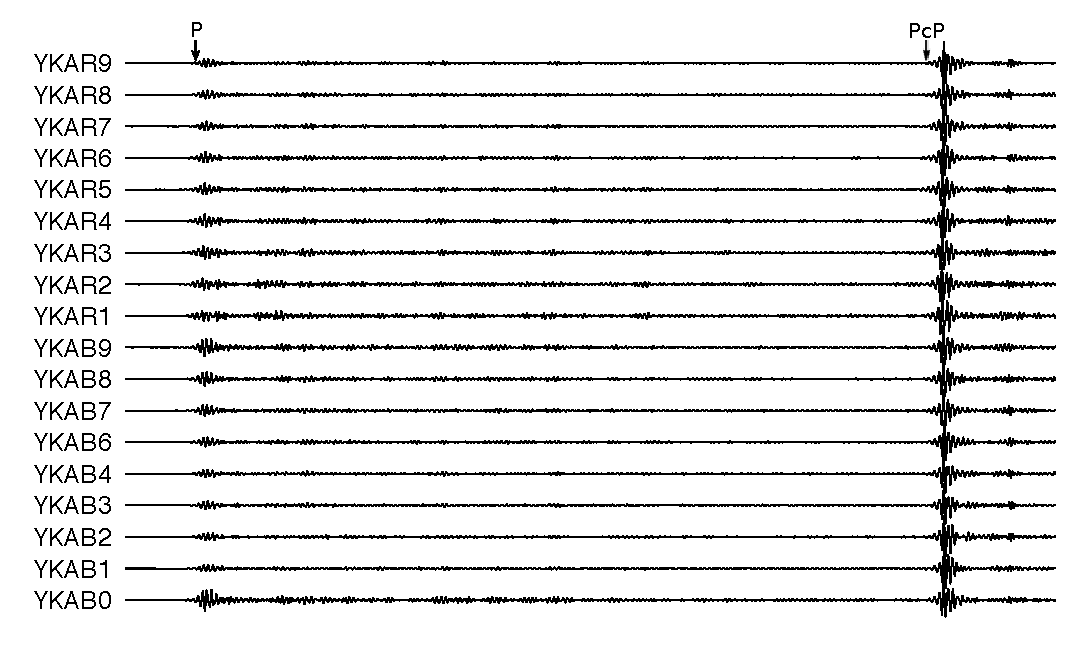
\includegraphics[width=0.87\linewidth]{fig/chap3/p_pcp_4599655.eps}
\caption{YKA对事件2014/04/21 14:02:15(Mw 
5.4, 54 km)产生的P和PcP记录. 每一道按照PcP振幅归一化, 可以明显看出台站间P波的振幅差异. }
\label{p_pcp}
\end{figure}

通过观察事件14、15每道记录的P和PcP振幅,可以发现即使在同一台阵内,台站间的P波振幅差异可以达到2倍,而PcP的振幅差异则很小,因此若将每道记录的振幅按照PcP振幅归一化,可以明显看出P波振幅的变化(图\ref{p_pcp}). YKA台阵位于稳定的克拉通岩石圈之上,其所处区域经受了稳定的沉积过程,所以这可能是由于台阵下方存在的沉积结构对P波的衰减,而PcP由于其相对小的慢度,受到的影响较小. 仅考虑这一点,使用P作为参考将为就会造成对CMB结构不正确的估计,以此使用PKiKP作为参考相就显得很有必要. 

\begin{figure}
\centering
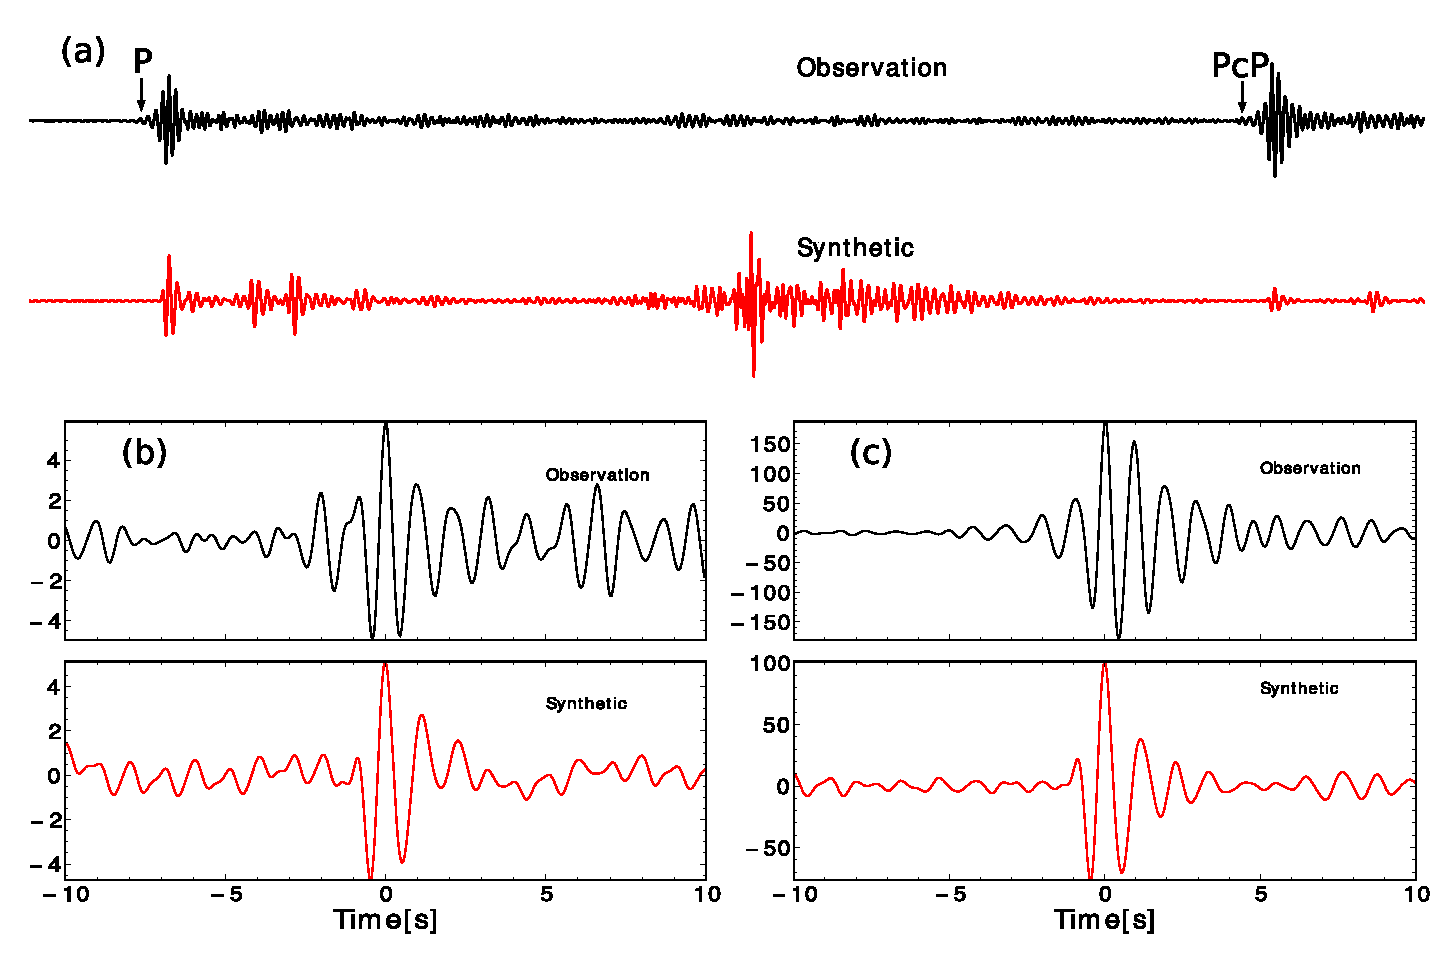
\includegraphics[width=0.85\linewidth]{fig/chap3/syn_2}
\caption{YKA台阵对表\ref{evt}地震14的记录和DSM理论地震图. (a)观测和理论的P和PcP的振幅比较;(b)观测和理论的PKiKP振幅比较;(c)观测和理论的PcP振幅比较. 其中观测记录来自台站YKB8. }
\label{fig:syn_2}
\end{figure}

\begin{figure}
\centering
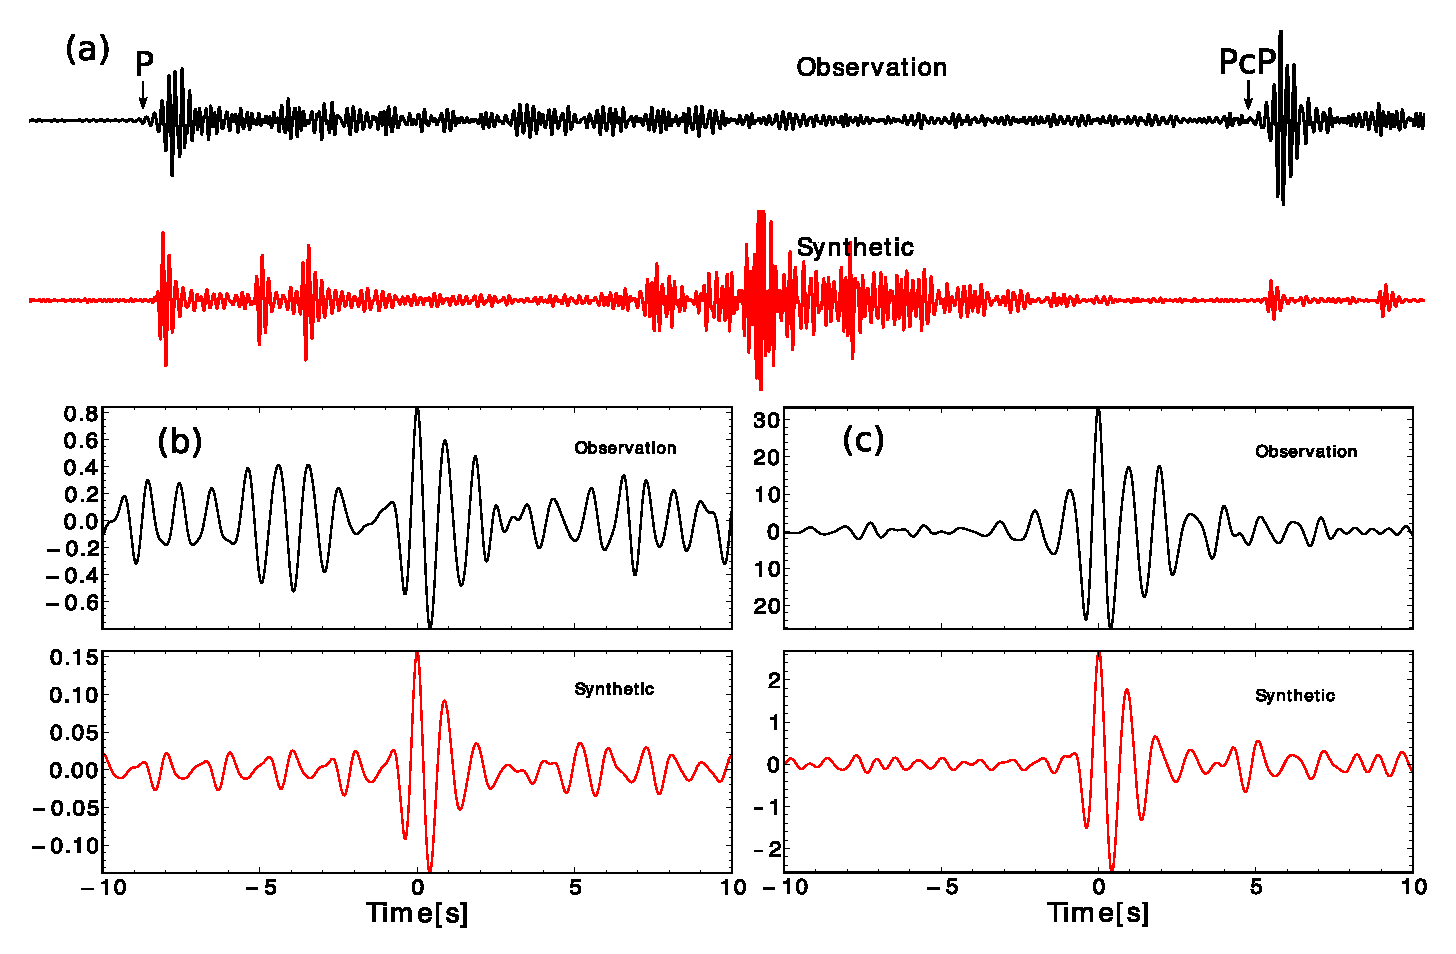
\includegraphics[width=0.85\linewidth]{fig/chap3/syn_3}
\caption{YKA台阵对表\ref{evt}地震15的记录和DSM理论地震图. (a)观测和理论的P和PcP的振幅比较;(b)观测和理论的PKiKP振幅比较;(c)观测和理论的PcP振幅比较. 其中观测记录来自台站YKAR9. }
\label{fig:syn_3}
\end{figure}

\begin{figure}
\centering
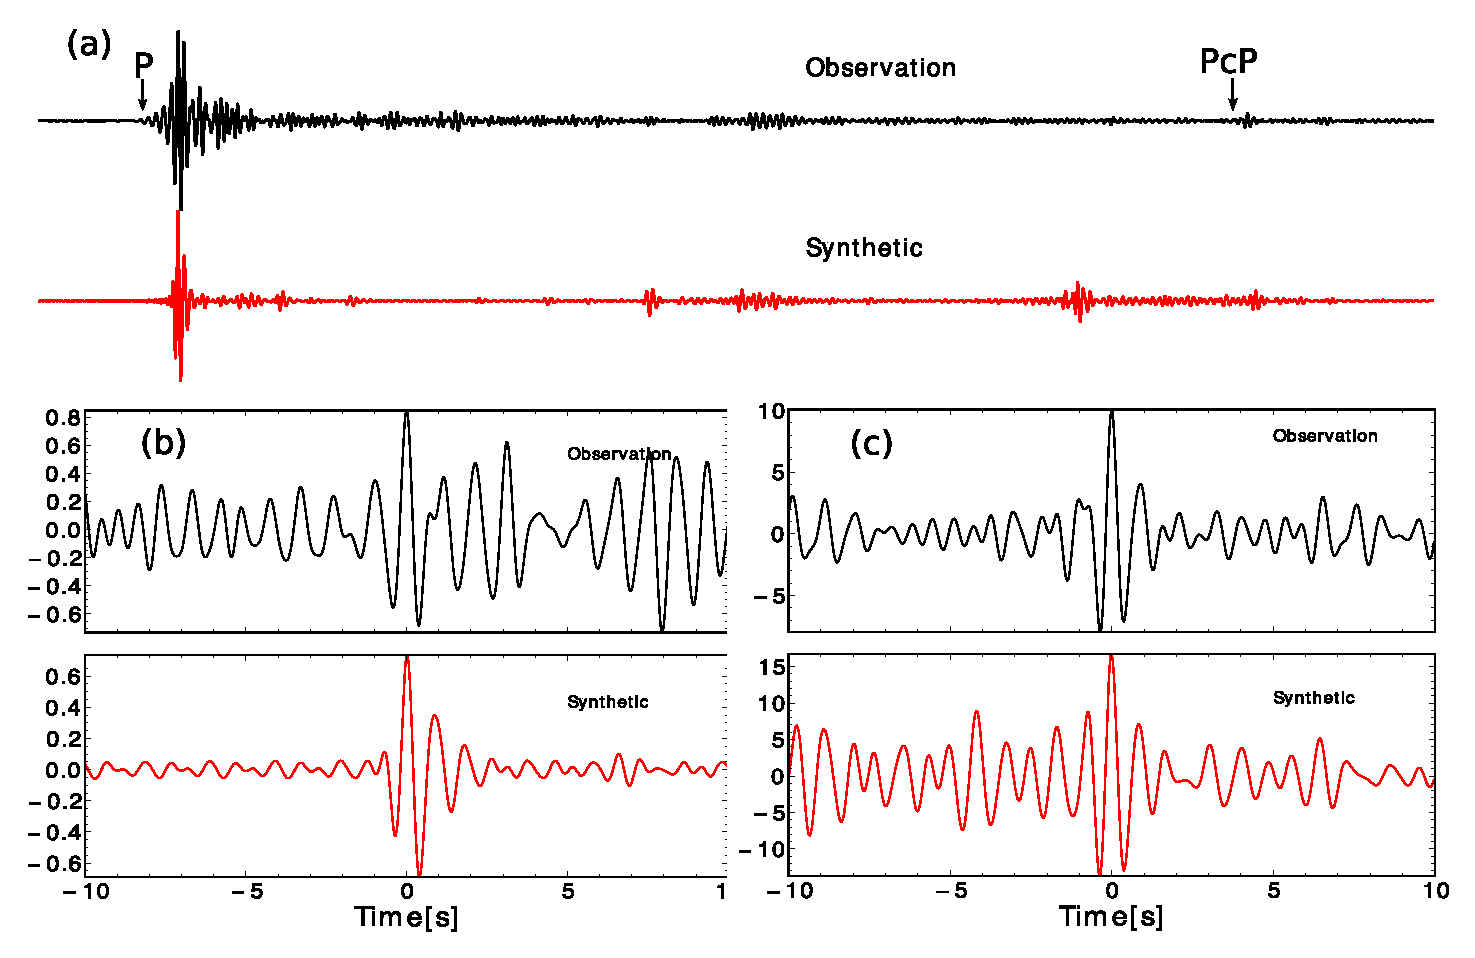
\includegraphics[width=0.85\linewidth]{fig/chap3/syn_1}
\caption{YKA台阵对表\ref{evt}地震13的记录和DSM理论地震图. (a)观测和理论的P和PcP的振幅比较;(b)观测和理论的PKiKP振幅比较;(c)观测和理论的PcP振幅比较. 其中观测记录来自台站YKAR9. }
\label{fig:syn_1}
\end{figure}

\begin{figure}
\centering
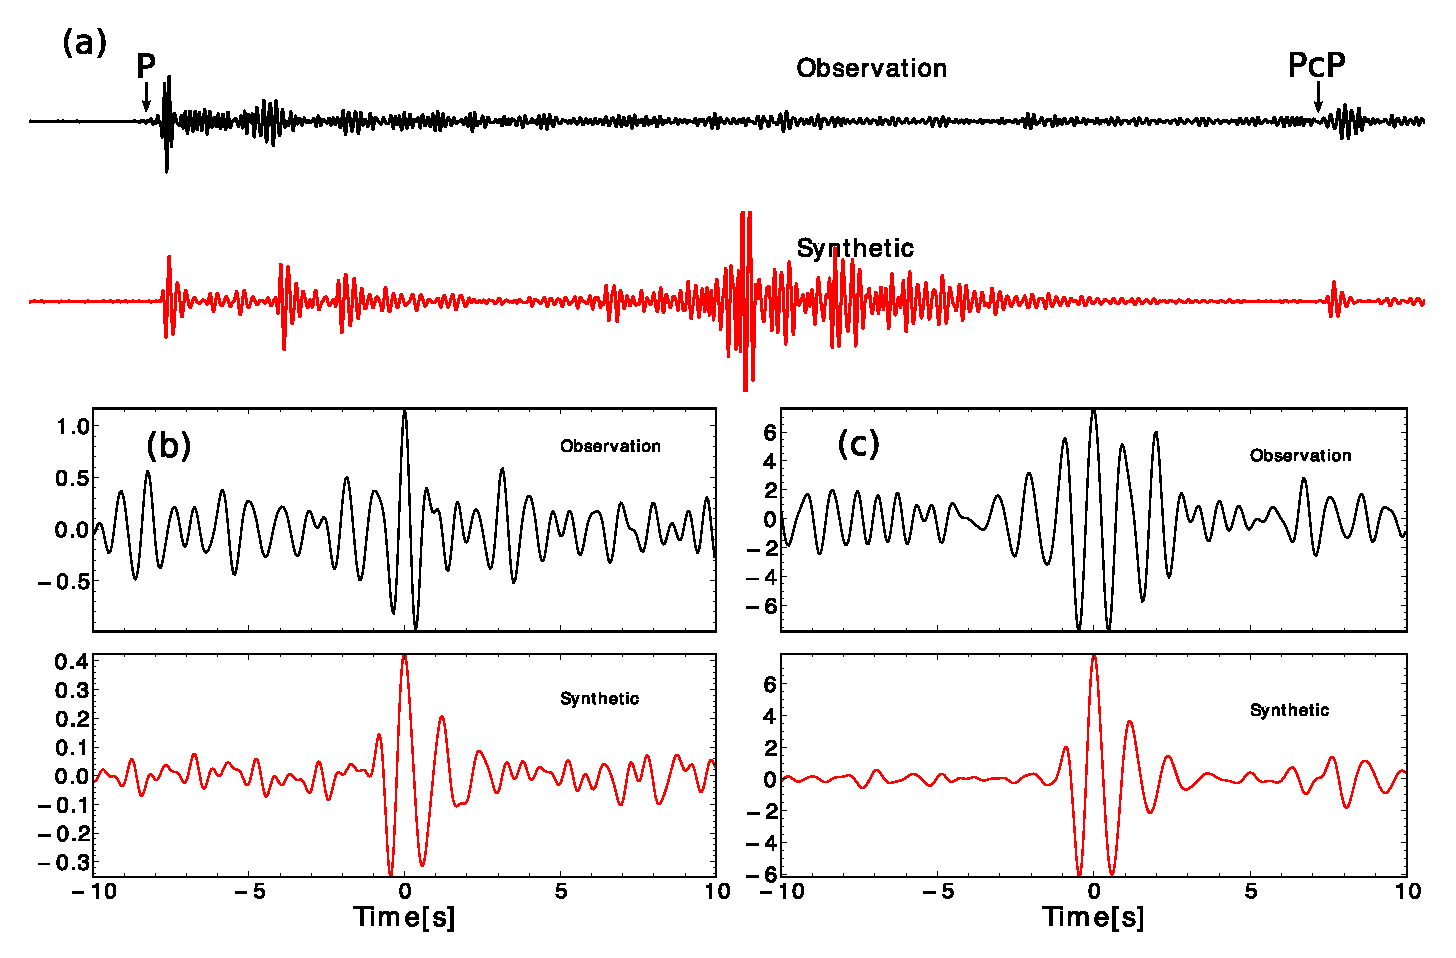
\includegraphics[width=0.85\linewidth]{fig/chap3/syn_4}
\caption{YKA台阵对表\ref{evt}地震16的记录和DSM理论地震图. (a)观测和理论的P和PcP的振幅比较;(b)观测和理论的PKiKP振幅比较;(c)观测和理论的PcP振幅比较. 其中观测记录来自台站YKR2. }
\label{fig:syn_4}
\end{figure}

为了消除震源对P、PcP和PKiKP振幅的影响,这里再使用DSM~\citep{Takeuchi1996,Kawai2006}计算理论地震图,将其与观测记录比较,进一步对PcP被放大的推测作检验. 为了尽量减小P波受台阵下方结构衰减对分析的干扰,所用的观测记录均选取台阵内具有最大P波振幅的台站记录. 可以发现,对于两个产生异常小振幅比的事件,DSM计算的PcP振幅比P波振幅小,与观测记录有很大差异,PKiKP/PcP振幅比也比DSM预计的要小一倍(图\ref{fig:syn_2},\ref{fig:syn_3});而对于
另外两个相邻地震,观测的的P/PcP振幅比并没有明显小于DMS预测的振幅比,反而PKiKP/PcP振幅比却比预测值
要大(图\ref{fig:syn_1},\ref{fig:syn_1}). 通过测量这七个事件的PKiKP-PcP相对PREM的差异走时
残差,也发现残差也恰好可以与一个Kenai半岛下方下凹的CMB对应(图\ref{fig:topo}b、c). 还
可以注意到,这7个地震的PKiKP/PcP振幅比和PKiKP-PcP差异走时残差之间存在一个正相关,这表明振幅比可能
与CMB或者ICB的起伏变化有所联系,而本研究更加倾向于前者,因为根据观测,PcP的变化要比PKiKP更加显著. 
观测到的Kenai半岛下方达到1.5秒的负走时残差也和之前的研究一致~\citep{Koper2004a,Waszek2015a},进一步验证了该区域走时残差测量的可靠性. 

在CMB处1$\sim$2Hz的PcP菲涅尔半径约为120km~\citep{Tkalcic2009},并且当CMB起伏的横向尺度和PcP的菲
涅尔带相当的时候,CMB起伏才会对PcP的振幅造成显著的影响~\citep{Wu2014a},因而图\ref{fig:topo}c中所描述的起伏尺度似乎也是比较合理的. 从7个地震的PcP-PKiKP差异走时残差的相对变化来看,观测值与标准模
型之间存在一个系统性的偏差,这可能是该区域下方的外核厚度有整体的变薄. 总而言之,所有的观测都支持该区域CMB存在一个局部下凹,但由于ICB的起伏变化仍然是未知的,而且走时残差仍然受地幔结构的影响,因此得到准确的界面起伏尺度仍然存在困难.

\begin{figure}
\centering
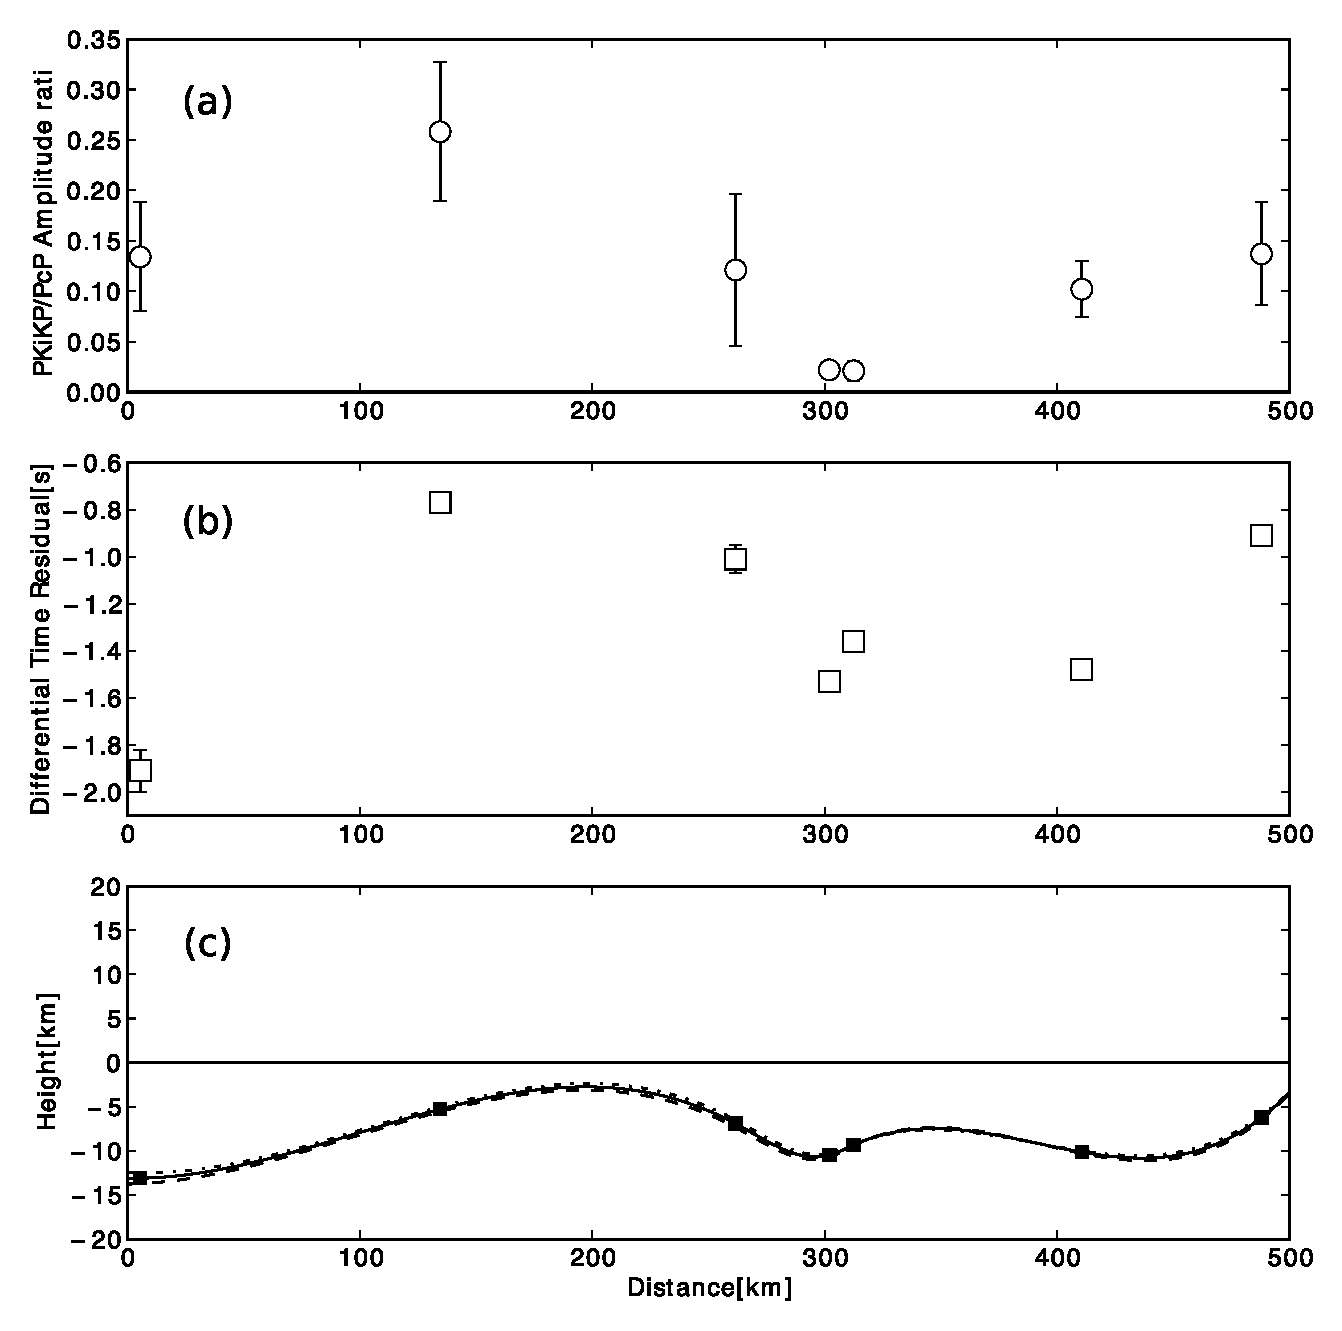
\includegraphics[width=0.7\linewidth]{fig/chap3/topo}
\caption{(a)YKA记录的图\ref{map}b中7个地震的PKiKP/PcP平均振幅比;(b)对应图\ref{map}c中反射点的PKiKP-PcP差异走时残差;(c)利用关系$H=\frac{t}{\sqrt{\frac{1}{V^2-p^2}}}$,可以将走时残差转换为深度变化,然后在插值得到界面的起伏变化. 点线和虚线表示应台阵走时残差的标准差. }
\label{fig:topo}
\end{figure}

由上面的观测,可以认识到CMB的起伏可能会出现比较复杂的情况,而产生这些复杂变化的则是复杂的外核和地幔的动力学过程. \citet{Lassak2010a}通过地球动力学模拟,认为地幔底部的物质堆积(Pile)和地幔柱在CMB起伏变化的形成过程中起到了重要作用. CMB上的物质堆积或地幔柱的上升流下方均对应CMB的隆升,而与俯冲板块相联系的下降流下方的CMB则呈现出凹陷. 但通过模拟难以将这两类模型的效应区分开,本研究所探测到的CMB小尺度界面起伏变化可能有助于缩小用于解释CMB结构变化的模型空间. 同时,形成当前地幔的速度结构和CMB起伏的动力学过程也不是相互独立的,通过地幔对流,它们可能存在相互耦合~\citep{Forte1991a}. 即地幔底部的速度异常和CMB的起伏存在某种对应关系~\citep{Forte1994a},如果将这种关系代入到地震波走时反演中就可以减少反演参数,从而得到更有物理意义的CMB模型~\citep{Soldati2012a}.

\subsection{ICB结构和CMB横向不均匀}

以上给出了两个用PKiKP和PcP分析CMB起伏变化的例子,但还有其他因素也会对振幅比和走时残差的观测造成影响,下面对一些主要的影响因素即ICB的结构和CMB横向不均匀性变化作一些讨论. 

\subsubsection{ICB结构}

对于前面的分析中并没有提及太多ICB效应对PKiKP/PcP振幅比和走时残差的影响,通常来说,其影响主要来自界面起伏变化及横向不均匀性变化. 如果这些变化比较显著的话,ICB的效应就不能忽略. 对于前面阿拉斯加的例子,除
了CMB局部凹陷的解释,观测到的异常小的PKiKP/PcP振幅比和大的负走时残差也可以被解释为一个局部上凸的ICB的效应(图\ref{fig:model}). 这样的一个ICB结构可以同时减小PKiKP走时和其振幅,导致负的走时残差和
小的振幅比. 如果是这种情况,PKiKP应该会出现与如图\ref{pcp_pkikp_nvpd}中PcP相似的波形变化,但实际上这并没有观测到,而且PKiKP在小于其菲涅尔半径的区域产生显著的能量发散也似乎是不可能的;另一方面,如果观测也可解释为ICB上局部速度和密度差的急剧降低,这种变化常被认为是ICB上方的小尺度对流的结果~\citep{Krasnoshchekov2005},但对于阿拉斯加的情况,相邻地震在ICB采样区域非常接近,因此出现这样变化的可能性很小,且PKiKP对这种10km级别的变化也不会太敏感. 对于NVAR和PDAR的数据,观测到的同一地震采样两个区域的ICB的PKiKP高度一致,因而ICB的效应可以忽略. 

\begin{figure}[!ht]
\centering
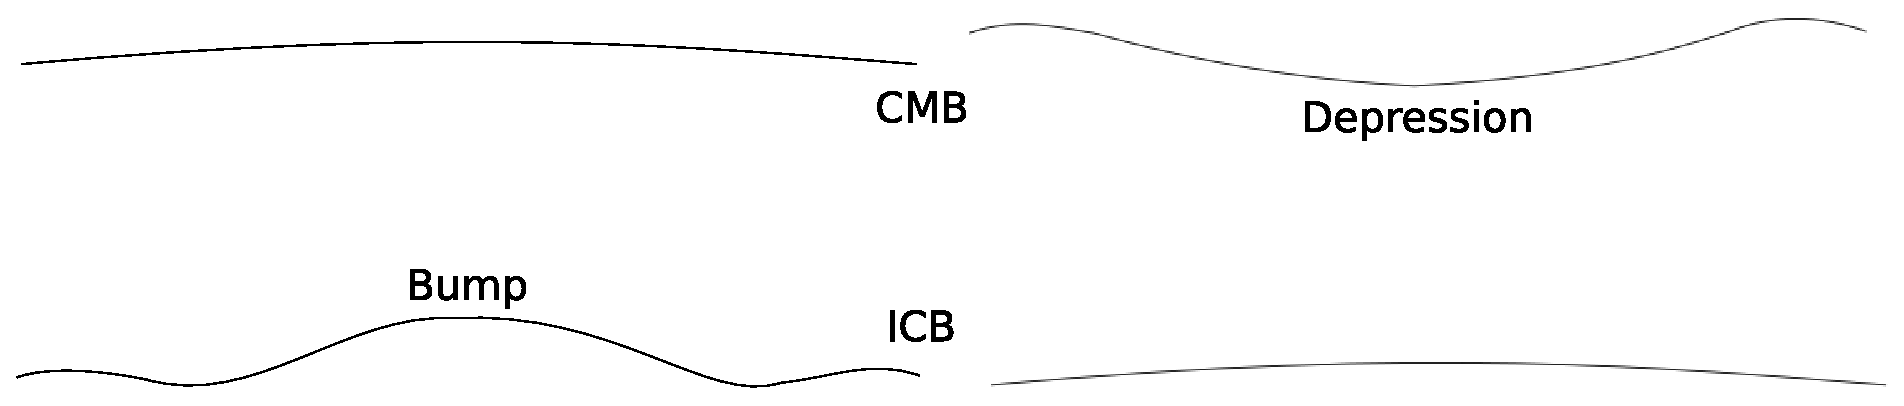
\includegraphics[width=0.7\linewidth]{fig/chap3/model}
\caption{两种可以解释YKA台阵PcP和PKiKP观测的CMB和ICB起伏模式,(左)下凹的CMB和平坦的ICB,(右)平坦的CMB和上凸的ICB. }
\label{fig:model}
\end{figure}

到目前为止,已经有一些研究给出ICB上存在小尺度起伏变化的证据. 其中一些研究使用间接方法,即基于内核差异
旋~\citep{Song1996}造成的ICB随时间变化,利用重复地震对产生的后临界PKiKP的变化来约束ICB起伏~\citep{Wen2006};一些使用前临界PKiKP观测来直接探测ICB起伏变化\citep{Dai2012}. 估计的ICB起伏的高度变化
从数百米~\citep{Cao2007}至数km~\citep{Dai2012},横向尺度也大约也是km的数量级. 对比ICB和CMB起伏的研究,似乎ICB的起伏程度要小于CMB,如果再考虑内外核差异旋转的效应,一个很高的ICB的上凸也是很难维持的. 因此本文认为仅ICB起伏不能完全解释所有的观测. \citet{Krasnoshchekov2005}引入了一种马赛克结构的ICB模型来解释PKiKP的剧烈振幅变化,这种类似补丁的结构由ICB上方薄的部分熔融液体和固体层交替组成,PKiKP在固体或液体层反射后的振幅会有显著不同. 之前的研究认为这种补丁结构是由与内核的不均一冷凝或者是ICB上方的物质对流所致,并估计这种结构的尺度从数十至数百km. 然而,在本研究中,小范围内剧烈的PKiKP振幅变化并没有被观测到,临近区域相同震级的地震产生的PKiKP振幅往往也是接近的,这也说明在本文的研究区域并没有这样的结构存在. 

\subsubsection{CMB横向不均匀性}

除了CMB的界面起伏,其物性的横向的不均匀也会对PcP的产生比较大的影响. 典型的超低速带(ULVZ)通常存在30\%的S波波速和10\%的P波波速的降低~\citep{Thorne2004a},这样的一个低速异常可以有效低降低50\%的PcP反射系数. 然而,仅用ULVZ并不能解释PDAR记录的PcP波形的变化(图\ref{amp_nv_pd}),并且之前的研究
并没有发现存在ULVZ的证据~\citep{Havens2001a}. 对于阿拉斯加的下方的CMB,虽然可能存在一个凹陷的地
形和高剪切波波速的折衷效应~\citep{Castle2000},但根据本研究的观测,异常小的PKiKP/PcP振幅比仅仅存
在于Kenai半岛的下方,因为尺度很小,如果将其认为突然的剪切波速度增高使PcP振幅增大,则很难说明其形成机制,因而解释为CMB局部的下凹显得更加合适. 除了本文提到的CMB起伏变化,前人的观测还显示出阿拉斯加下方地幔底部存在3\%的各向异性,即水平极化的S波比垂直极化的S波快3\%,其与上覆地幔的各项异性差异形成了D''不连续面~\citep{Matzel1996a};并且还有研究发现在该区域存在异常的P和S波波速比,同时两者呈现反相关,这可能暗示阿拉斯加下方的CMB存在某种物质组分的异常~\citep{Wysession1999a}. 异常的来源可能是硅质地幔与液态铁合金的化学反应的产物~\citep{Jeanloz1993a}. 这些可能的CMB上方的结构异常与Kenai半岛下方的CMB起伏有何种联系,还需要今后进一步的研究.

\section{CMB上方的低速结构}

\begin{figure}[ht]
\centering
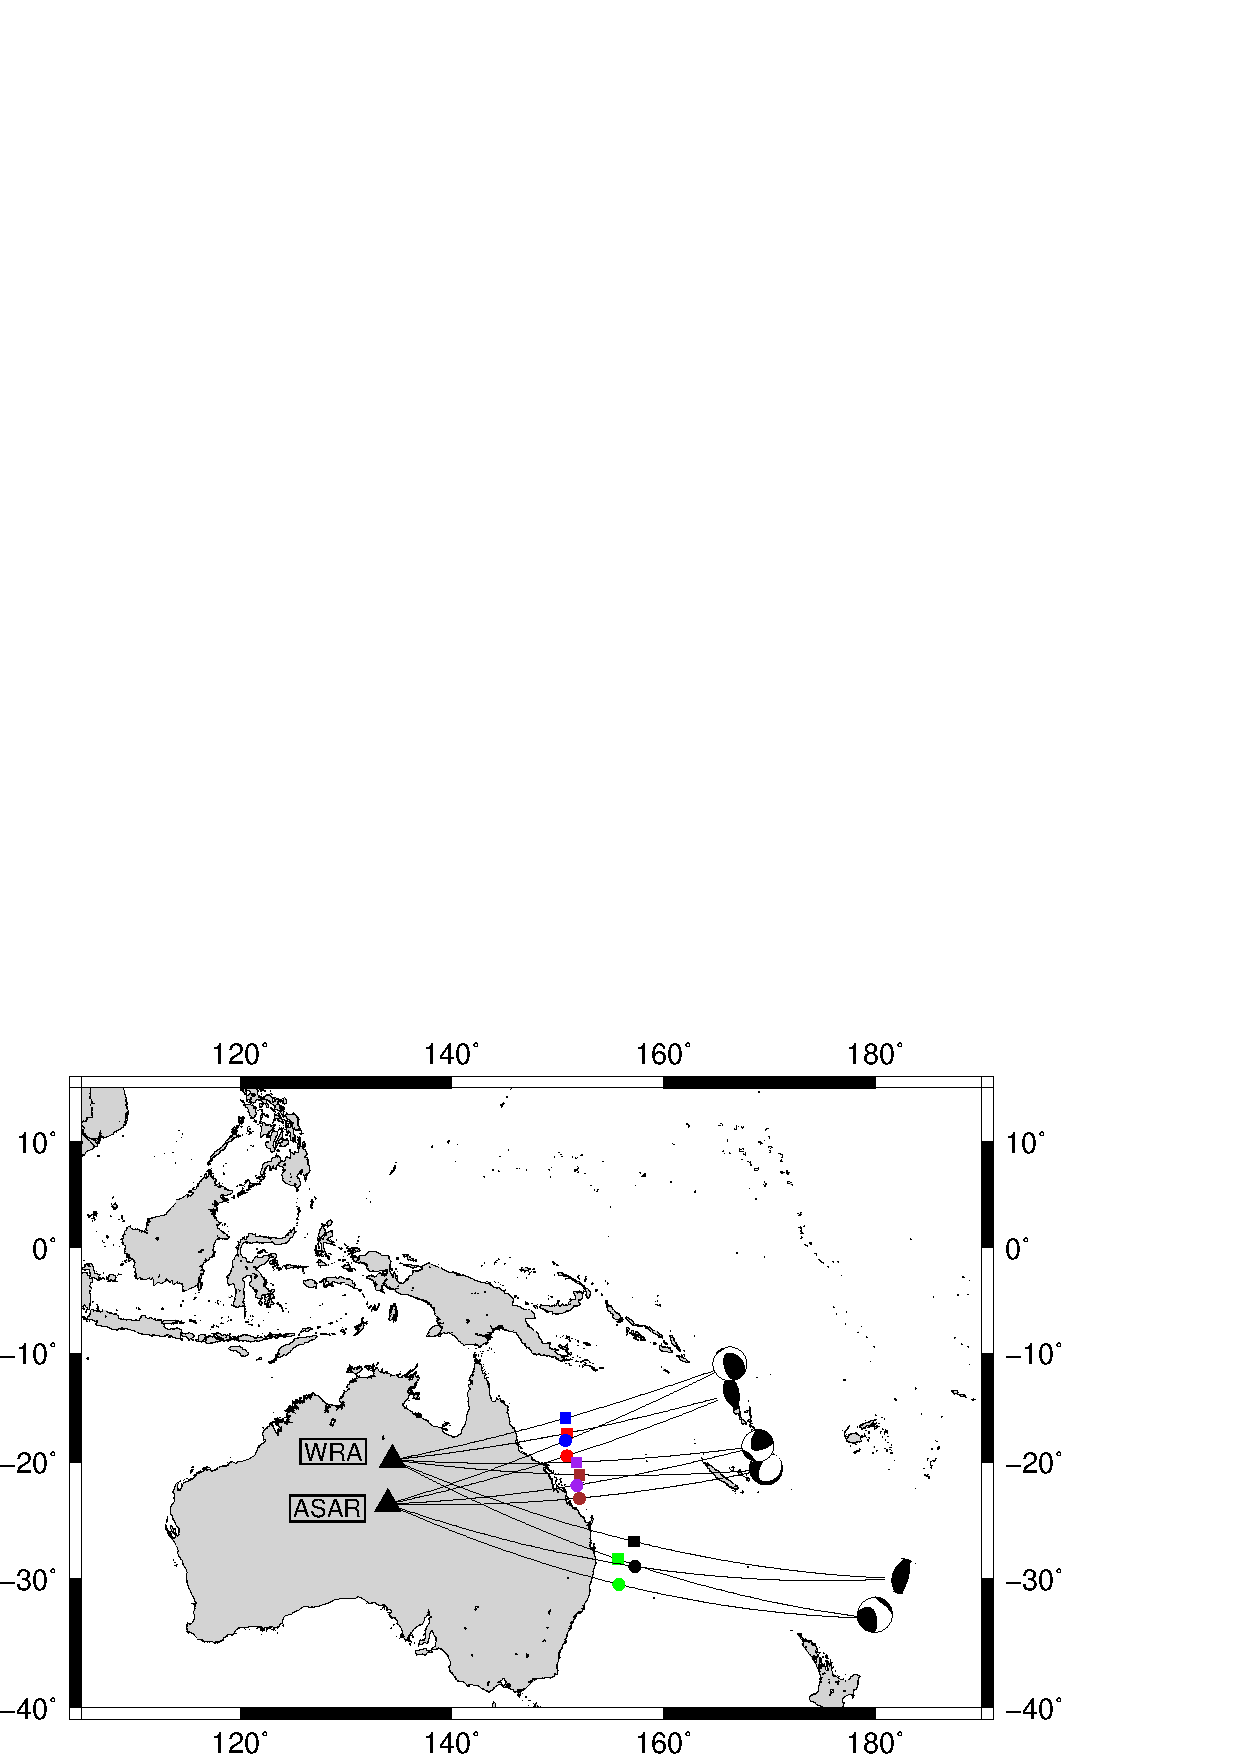
\includegraphics[width=0.8\linewidth]{fig/chap3/evt_au}
\caption{位于澳大利亚中部的WRA和ASAR台阵及表\ref{evt}中第18--23号事件的位置. 黑色三角形表示台阵位置,黑色连线表示地震到台阵的路径. CMB反射点位置用彩色方框和圆圈表示,方框代表WRA,圆圈代表ASAR,每种颜色代表一个地震. }
\label{fig:evt_au}
\end{figure}

前面一节主要分析了CMB界面起伏对PcP、PKiKP/PcP振幅比和PKiKP-PcP走时残差的影响,这一节就CMB上部低
速结构特别是ULVZ结构对观测振幅比和走时残差的影响进行探讨. 结合\citet{McNamara2010}总结的前人对全球范围内超低速带的观测和全球IMS小口径台阵的分布情况,能采样到前人研究所发现的CMB超低速带的只有位于澳大利亚的WRA-ASAR台阵对的数据. 因此,这一节利用对这两个台阵的PcP和PKiKP数据,分析CMB低速或ULVZ结构对PKiKP/PcP振幅比异常的贡献;同时,结合PKiKP-PcP走时残差分析所采样区域的界面起伏变化. 

这里一共选取6个地震事件,其中四个分布在圣克鲁兹群岛至瓦努阿图群岛之间,另外两个位于新西兰的克马德克群
岛. 对于前四个地震,两个台阵到它们的震中距基本在31{\textdegree}--32{\textdegree}之间,PcP反射
点位于CMB上$-$23{\textdegree}S至$-$16{\textdegree}S的位置,8个反射点位置经度变化不大,在CMB
上近似地排成一条线状剖面,并恰好位于\citet{Thorne2004a}利用SKP${}_{diff}$S探测到的ULVZ附近,
并位于\citet{He2012a}所定义的“太平洋异常”西边界上;台阵到其余两个地震的震中距约42{\textdegree}--44{\textdegree},PcP反射点在CMB上$-$30{\textdegree}S附近,在“太平洋异常”西南边界稍稍偏下的
位置. 

\begin{figure}
\centering
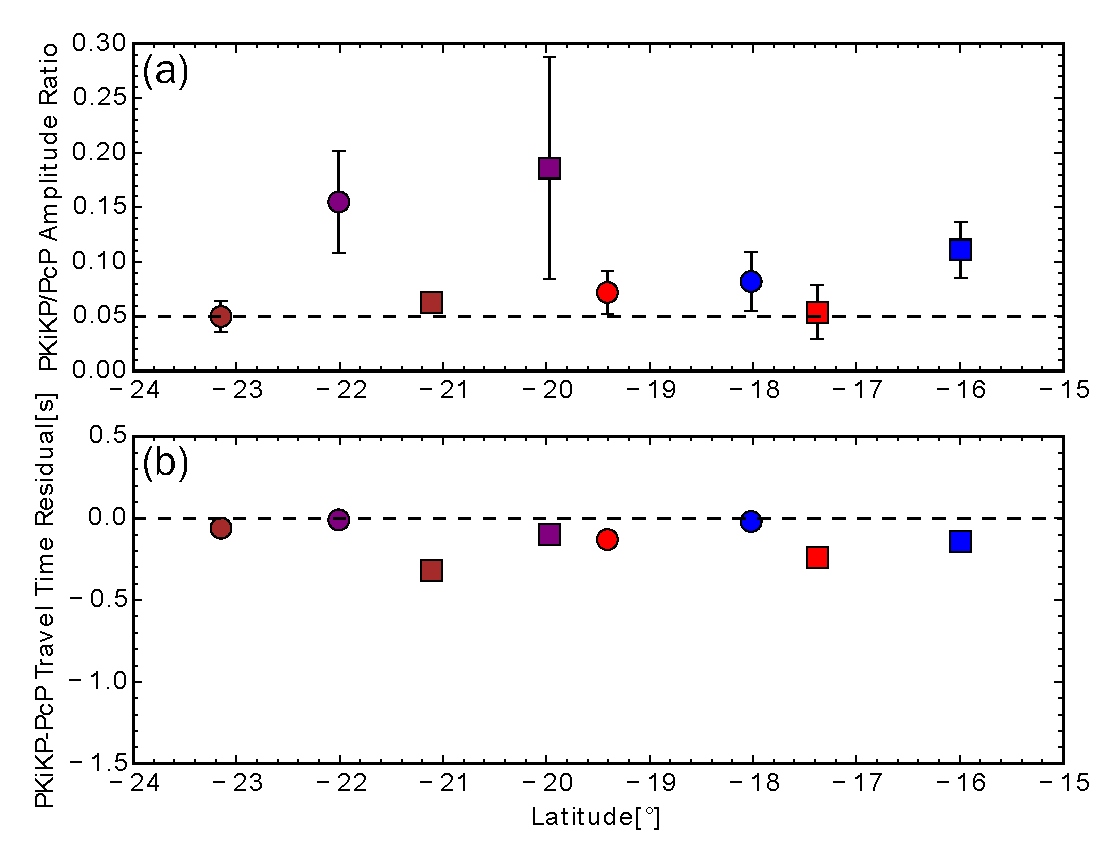
\includegraphics[width=0.7\linewidth]{fig/chap3/au_ratio_tres}
\caption{(a)图\ref{fig:evt_au}中事件-台阵对的PKiKP/PcP振幅比,每个观测点的颜色和形状图\ref{fig:evt_au}中的颜色形状对应. 虚线表示震中距30{\textdegree}时PREM预测的振幅比;(b)每个事件-台阵对的PKiKP-PcP相对PREM的走时残差,颜色表示同(a). 虚线表示走时差于PREM零偏差的位置. }
\label{fig:au_ratio_tres}
\end{figure}

WRA和ASAR仅距离400km,而且每个相邻地震-台阵对的PcP反射点在CMB距离大多在60km左右,有的甚至只有30km,因此比起距离1000km的NVAR和PDAR,这两个台阵更适合探测CMB小尺度的变化. 本研究首先对前四个地震的
数据进行分析,尝试估计CMB变化的横向尺度. 首先看图\ref{fig:evt_au}中连续8个反射CMB反射点的位置,
每个事件相应的反射点相互交错,这样就使得不同事件-台阵对的振幅比和走时残差可以互相参考. 8个事件-台阵对
的平均振幅比显示(图\ref{fig:au_ratio_tres}a),对于同一个地震,WRA和ASAR的平均PKiKP/PcP振
幅比基本上比较接近,这说明两个台阵数据采样到的CMB结构是相似的;褐色和红色表示的反射点对应的振幅比也大
致接近,约为PREM预测值的1.5--2倍左右,而圣克鲁兹群岛事件对应的振幅比均稍稍偏大,但ASAR的振幅比较WRA
的小一些;比较异常的是紫色表示的Vanuatu事件,其振幅比平均值远大于相邻两个CMB采样点的,但可以注意到,平均振幅比的标准差也非常大.由于相邻采样点对应的振幅比并不存在特别大的异常,这里可以推测过大的振幅比并非是CMB或者ICB结构变化造成的. 

与振幅比的局部突然增大相比,走时残差却显得非常稳定,所有的事件-台阵对均显示出微负的走时残差,相邻CMB采样点对应的残差的差别最多不超过0.3秒. 值得注意的是,由ASAR观测到的走时残差都接近零,而对于同一地震,相应的WRA观测总是稍稍偏大约0.1--0.3秒,这表明WRA数据可能存在某种系统性的偏差,比较合理的解释是在WRA台阵侧PKiKP和PcP经历了不同的速度结构,假设这种情况成立,那么由CMB起伏引起的走时残差变化就会更小,因而可以认为采样区域的CMB是比较平坦的,估计的起伏上限也只有数百米,这与之前利用ScP研究CMB起伏的研究结果相似~\citep{Vidale1992a}. 

\begin{figure}[ht]
\centering
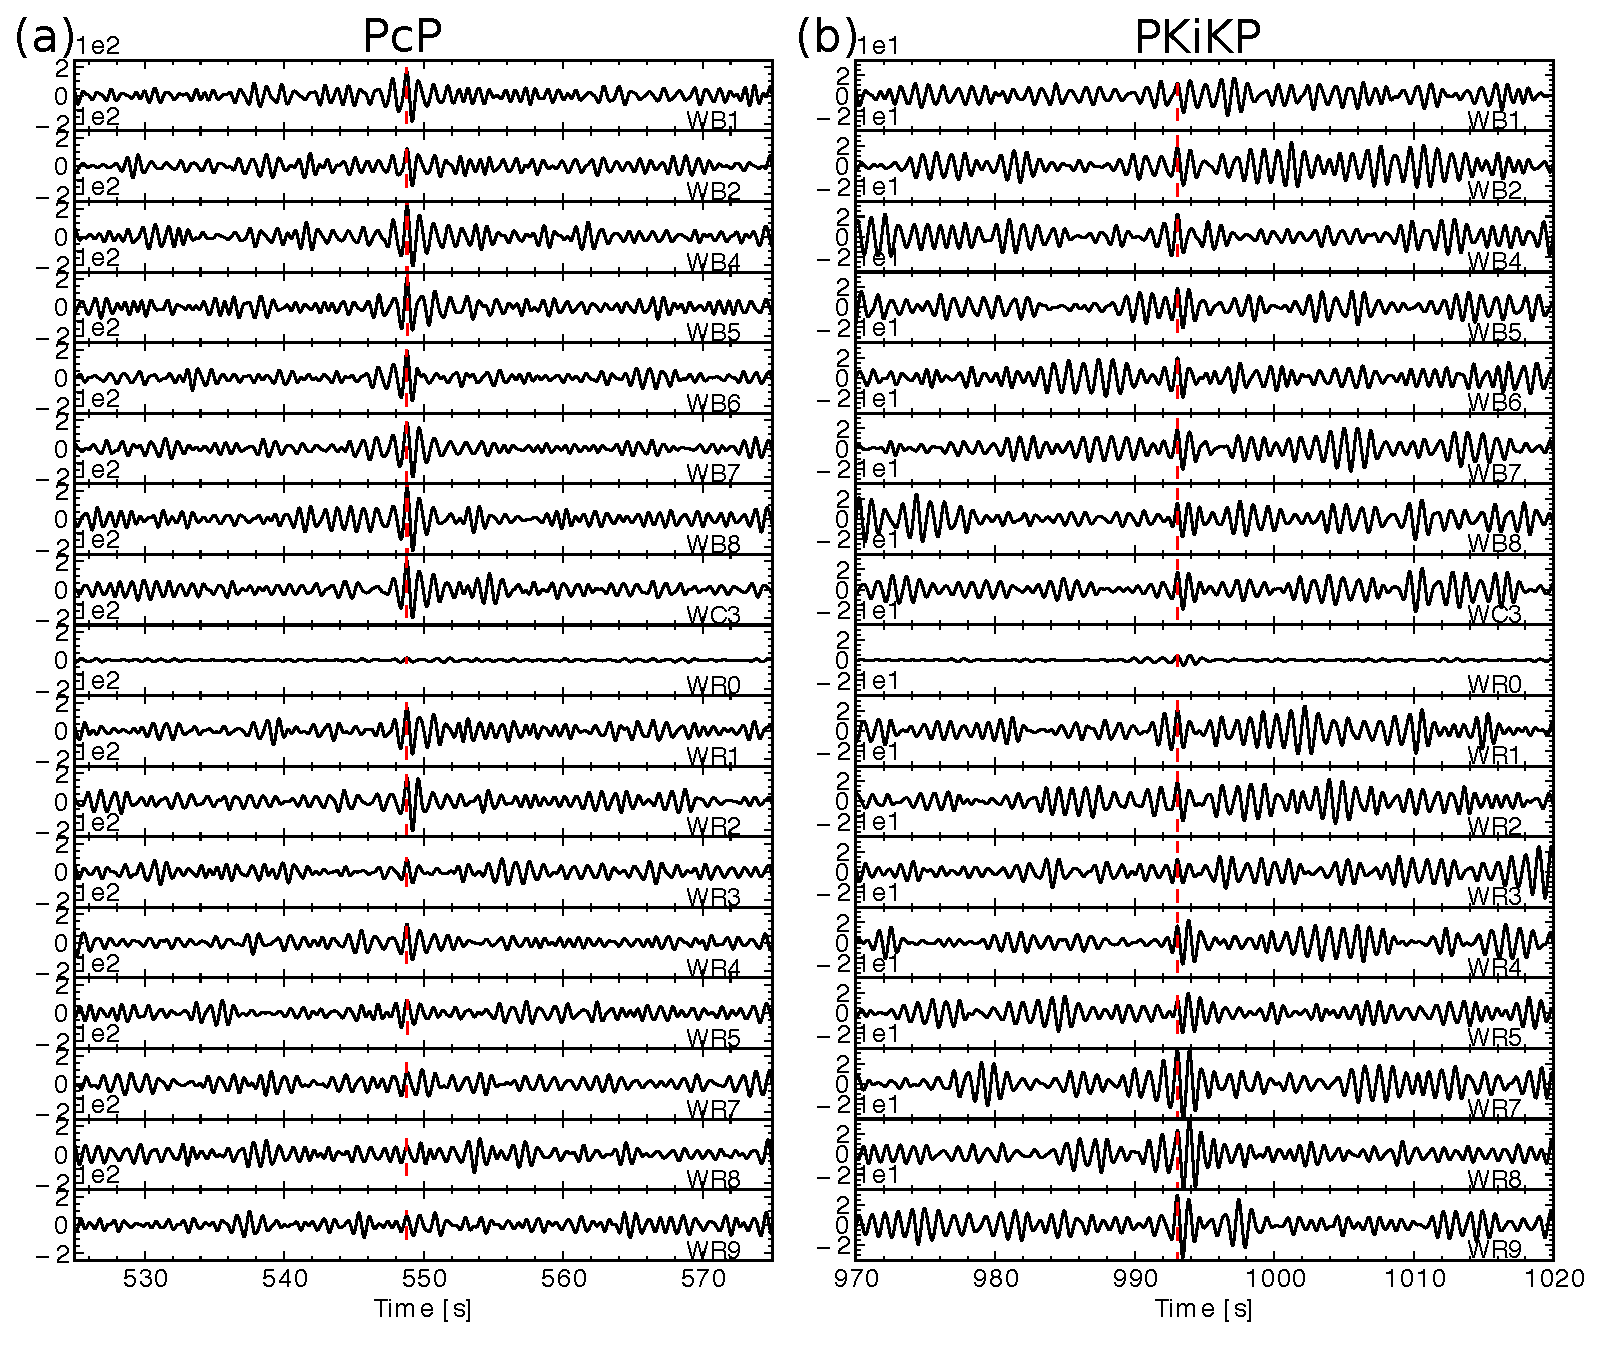
\includegraphics[width=\linewidth]{fig/chap3/pcp_pkikp}
\caption{WRA对表\ref{evt}中第22号地震的PcP(a)和PKiKP(b)记录. 红色虚线标出测量的PcP和PKiKP振幅峰值位置. }
\label{fig:pcp_pkikp}
\end{figure}

再回到PKiKP/PcP振幅比的问题上来. 根据走时残差的结果,推断采样的CMB区域是比较平坦的,那么造成振幅比
突然变化的因素便不会是CMB起伏,可能是由于震源的因素,即在离开震源后,PcP立刻受到较大的衰减,通过比较
震源深度,发现产生振幅比较大的事件震源深度达到200km,可能受到俯冲板块的影响,造成异常的振幅比观测. 虽然台阵记录的不确定性也会造成很大的平均振幅比和标准差,但两个台阵呈现一致的变化,因此可以排除台阵本身的因素. \citet{Koper2004a}在此区域也同样观测到很多异常大的PKiKP/PcP振幅比,但这里并没有发现很多类似的情况,之前研究大振幅比的观测可能是台阵内台站记录存在较大差异的结果,如图\ref{fig:pcp_pkikp}显示的WRA对事件22的PcP和PKiKP记录,所有的台站记录全都按照相同振幅尺度画出,可以发现很多WRX台站记录的PcP振幅要明显偏小,而PKiKP则明显偏大了,这样单道的振幅比就会明显增大. 之前研究通常采用的是所有记录的叠加后的振幅比,即把那些振幅比很大的记录也包含在内了,因此可能得到一个虚假的振幅比异常. 还是以图\ref{fig:pcp_pkikp}的记录为例,如果包含所有WRX台记录,得到的平均台阵振幅比将超过0.25,当舍弃这些小PcP的记录,平均振幅比立刻降到0.1之下(图\ref{fig:au_ratio_tres}a中的褐色方框),且标准差也大大减小了. 通过以上分析,可以认为某些观测到的异常大的振幅比并不是CMB变化所造成的,震源一侧的结构可能对此有很大的贡献,这也可以解释两个台阵振幅比观测的一致性. 除此之外也不能排除过大的振幅比是不正确的震源校正造成的~\citep{Rost2004a},在小震中距情况下,虽然PcP和PKiKP的离源角相差不大,但当它们的出射位置接近辐射花样的节平面的时候,两者的能量可能有显著差异.

%采样区域恰好处于以往研究所定义的超低速带附近,而关于西太平洋低速异常边缘的超低速带研究显示S波波速可以
%达到13\%的降低~\citep{He2006a,He2012a},即使不考虑比较极端的30\%的情况~\citep{Thorne2004a},用ULVZ也足以解释振幅比大于PREM预测一倍左右的观测(图\ref{fig:model_cmb}). 

\begin{figure}[ht]
\centering
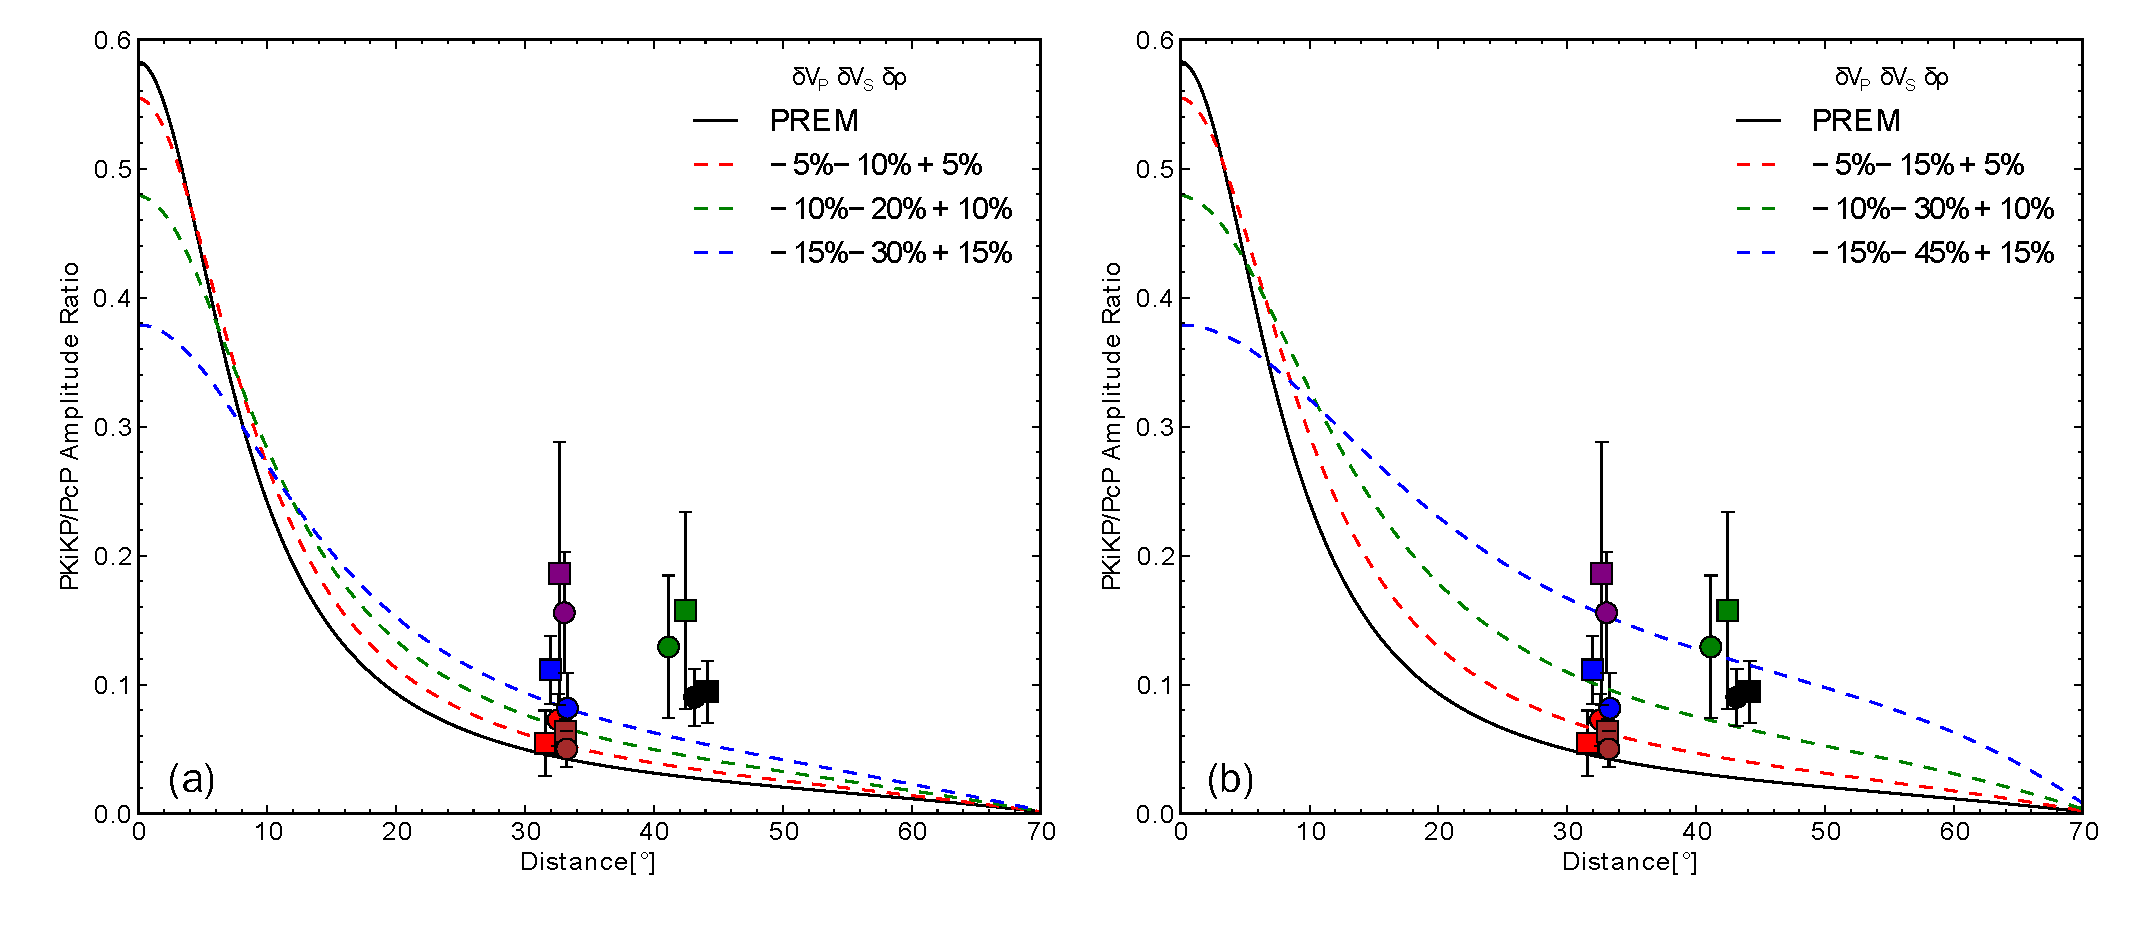
\includegraphics[width=1\linewidth]{fig/chap3/model_cmb}
\caption{不同ULVZ模型参数下的理论PKiKP/PcP振幅比曲线和观测振幅比. (a)$\delta$V${}_P$:$\delta$V${}_S$=1:2,波速的减小和密度的增大以整数倍增加;(b)$\delta$V${}_P$:$\delta$V${}_S$=1:3,参数变化方式同(a). }
\label{fig:model_cmb}
\end{figure}

由于采样区域恰位于前人定义的ULVZ附近,关于西太平洋CMB低速异常边缘的研究显示CMB底部S波波速可以降低13\%~\citep{He2006a,He2012a},假设实际的ICB物理参数与PREM描述一致,则本文观测到的振幅比中的较小值可以和之前的研究结果相吻合(图\ref{fig:model_cmb}),除了异常的大振幅比,图8中稍大的振幅比可能需要用20\%至30\%的S波波速降低来解释. 对于位于“太平洋异常”西南边界之外的两个采样点对应的振幅比,可能还需要用更大的S波波速降低来解释(大于30\%). 考虑到观测的不确定性,仅用PKiKP/PcP振幅比仍然不能很好地约束CMB参数,这里的结果也仅能为之前的研究提供一些支持,同时也体现出用振幅比研究界面参数的局限性. 还可以注意到,采样“太平洋异常”西边界的PcP波形与PKiKP相似,主反射震相之前并没有出现明显的信号,这说明即使超低速层是存在的,这一层的顶部也并非是一个不连续界面,或者层的厚度很薄,小于PcP的波长(约13km),不足以产生可观测到的反射波,这也与之前利用ScP的研究该区域ULVZ厚度的结果相吻合~\citep{Rost2010a}.


\chapter{东亚下方CMB结构}

本章主要利用国家测震台网的PKiKP/PcP振幅比和走时残差数据,简要分析中国下方CMB的结构变化. 首先,前一节通
过振幅比和走时残差分析,研究CMB的中型尺度范围的变化;后一小结通过对比相同台站对两个不同时间,震级不同,但位置和震源深度都很接近的两个地震的PKiKP和PcP观测结果,讨论引起振幅比观测波动的因素. 

\section{振幅比和走时残差分析}

第二章中提到,利用国家测震台网,本研究发现了两个产生超过500个单道可识别的PKiKP信号. PcP和PKiKP的反射
点分别覆盖了中国西南和东北部下方的CMB和ICB上大约20{\textdegree}$\times$20{\textdegree}的区
域,记录的震中距接近40{\textdegree}(图\ref{cn_2011},\ref{cn_2013}). 虽然记录到如此多的PKiKP信号,但按照本研究的标准,实际可用的台站数据就不多了. 首先,对于2011年的地震,清晰PcP的观测质量
整体不高,且数量要远远小于PKiKP的;而对于2013年地震,绝大多数的台站PcP均比较清晰,少部分台站记录的
信噪比甚至超过10. 这种PcP的记录差异可能源于受S波尾波干扰程度的差异,中国西南下方的地幔结构可能比东北
下方的更复杂. 其次,每个台站的信噪比可能有很大差异,如果测量全部记录的PKiKP/PcP振幅比,会发现数据分
布非常离散,这样也会给分析带来极大的困难,因此为了减小离散,丢掉不确定性大的数据,进一步的数据挑选和数
据质量控制就很有必要. 

与IMS台阵不同,本研究对所有的挑选出同时含PcP和PKiKP信号的国家测震台网的台站记录再作如下两步筛选:(1)剔除信
噪比低的记录. 这里要求PcP和PKiKP的信噪比均大于2.5;(2)单道记录中PcP和PKiKP波形的相关系数大于0.9. 这也符合一个简单CMB和ICB的理论计算结果,如果两者波形比较相近,说明PcP和PKiKP都没有受到太大的干扰,因而适合用于振幅比的分析. 按照以上标准,对2013年事件,共挑选出119道记录;对2011年事件,挑选出59
道记录. 为了更好描述振幅比相对于PREM预测的偏差,这里采用\citet{Koper2004a}所定义的PKiKP/PcP对数振幅比残差(LARR),

\begin{equation}
LARR = \log 10 \left[\left(\frac{A_{PKiKP}}{A_{PcP}}\right)_{obs}\biggl/\left(\frac{A_{PKiKP}}{A_{PcP}}\right)_{prem}\right]
\end{equation}

同时计算挑选出记录的PKiKP-PcP走时残差,得到的图\ref{fig:bp_amp_res}中的结果. 从两次地震的PKiKP/PcP振幅比对数残差来看(图\ref{fig:bp_amp_res}a、c),可以发现某些相似的特征,即LARR都存
在比较明显的区域性差异. 2009年事件CMB上103{\textdegree}E以东的反射点大多都呈现稍大的正LARR,而靠近震源一侧,对应震中距从0至20{\textdegree}的反射点的振幅比则基本与PREM预测结果一致,其中有偏小的振幅比可能是由较低的PKiKP信噪比造成(表\ref{repeat_obs});2013年的事件,距离震源较近的,对应震中距小于25{\textdegree}反射点,显示出偏低的振幅比,PREM预测大约为观测的1.5倍左右,而其CMB西南方向一侧,也大多呈现较大的正LARR. CMB上138{\textdegree}E,48{\textdegree}N附近,可能存在某种过渡,存在由负到正的LARR变化. 观察这两个地震PKiKP-PcP的走时残差,再与LARR的分布比较,可以看出两者之间也存在明显的对应关系. 不论对哪个事件,较小的振幅比对应小的负走时残差,较大的正LARR和走时残差则出现相反的对应关系(图\ref{fig:bp_amp_res}(b)、(d)). 所有测量的走时残差均为负,绝大多数在2秒左右,最小的也接近1秒,表明中国下方的外核厚度存在明显的变薄,本研究的走时观测也和\citet{Shen2016a}在中国东岸下方的观测结果相吻合. 但在较小尺度的范围(约200km)内,走时残差的变化则很小,约为0.1秒的量级,这也暗示在小范围内,东亚下方的CMB起伏是不大的.

\begin{figure}[ht]
\centering
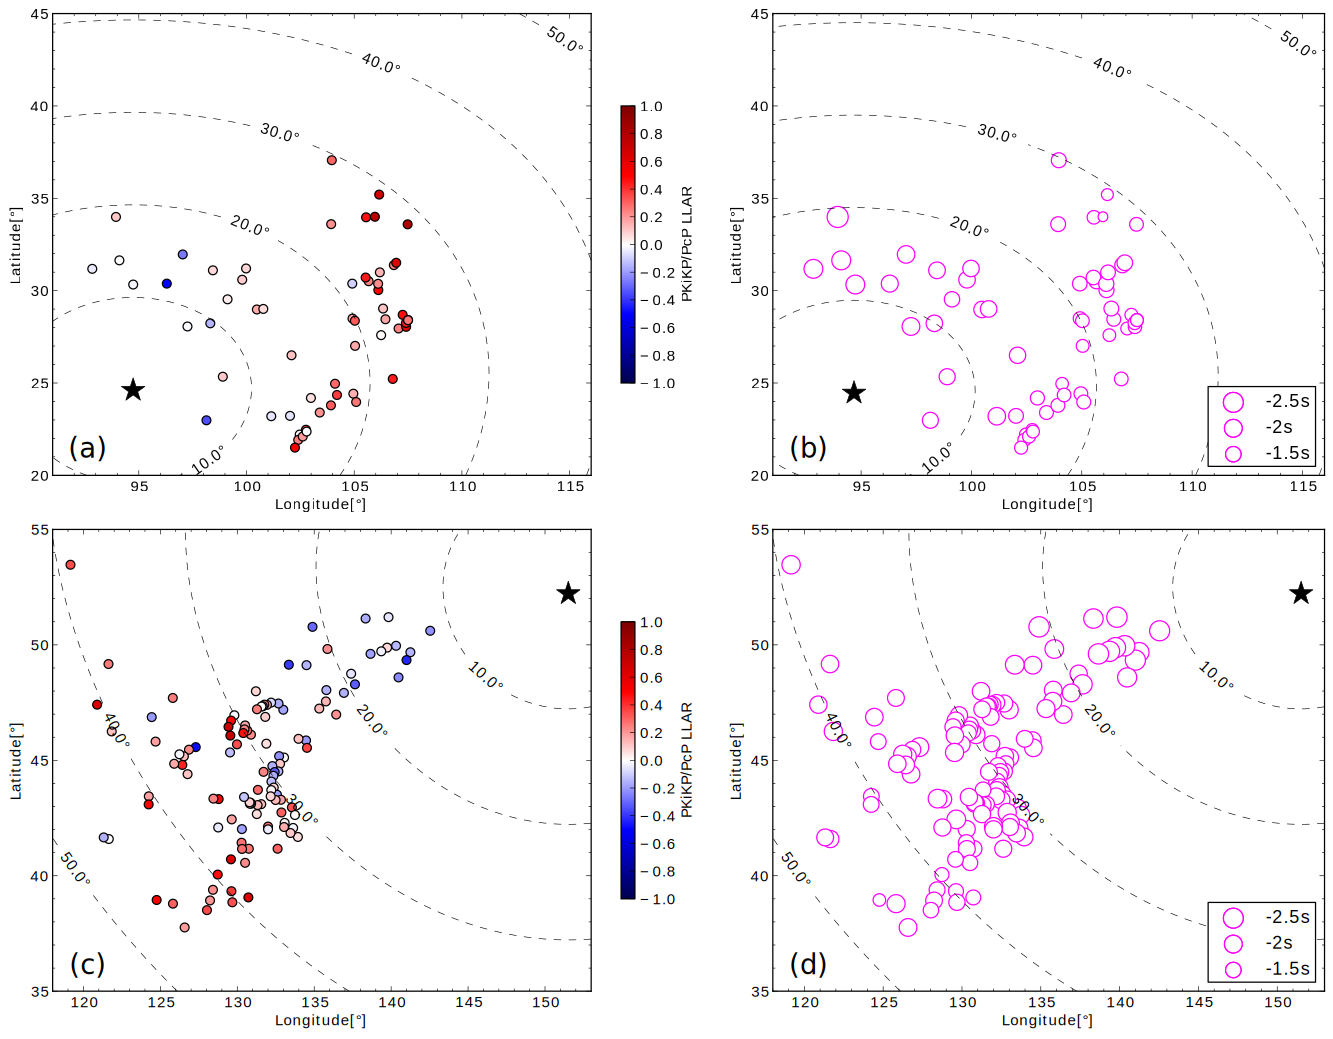
\includegraphics[width=\linewidth]{fig/chap4/bp_amp_res}
\caption{(a)、(b)事件2011/02/04(文中简称事件A)的PKiKP/PcP相对与PREM的对数振幅比残差和PKiKP-PcP走时残差分布;(c)、(d)对应事件2013/05/24(文中简称事件B)的结果,其余与(a)、(b)一致.图中的黑色五角星表示地震位置,等值线表示CMB上反射点对应的震中距位置.}
\label{fig:bp_amp_res}
\end{figure}

观察到的走时残差和LARR的正相关性和上一章所述及阿拉斯加Kenai半岛的情形一致,仅是尺度略微增大,因此也暗示了PKiKP/PcP振幅比受到了界面起伏变化的影响. 但这究竟是源于CMB的起伏还是类似\citet{Shen2016a}所提到的黄海周围ICB的界面起伏变化,还需要进一步讨论.

如前面提到的,对于事件A,在震中距10{\textdegree}到20{\textdegree}范围内观测的LARR
接近零,这就说明PREM就已经可以很好地拟合观测结果了. 因此,如果假定这部分区域的CMB和ICB的波速与密度
变化是PREM所描述的,而且该LARR“正常”区域的2秒走时残差负异常可以认为是中国下方背景外核厚度与PREM的
偏差,那么其东侧的LARR正异常和1~1.5秒的走时残差负异常就可以被认为是外核厚度的加厚,可能是CMB的局部
隆升造成的PcP振幅减弱或者是ICB的局部下沉造成的PKiKP振幅放大(图\ref{fig:model}). 假设是ICB的地
形下陷,那么这里的观测就要求ICB至少存在横向尺度为200km的起伏变化,但之前没有任何研究揭示ICB存在这样
的起伏尺度,而且就此事件而言,观测数量而言PKiKP要远远多于PcP,且超过40{\textdegree}震中距仍然有
清晰PKiKP的观测,这显示在大范围内ICB是稳定的、变化较平缓的. 对界面起伏来说,有下陷就必然有隆升,但就
本研究数据采样范围内,没有发现超过30{\textdegree}震中距出现增大的负走时残差;类似地,对于事件B,CMB上140{\textdegree}E,50{\textdegree}N附近可能存在一个平缓的局部下陷,因为此处的
走时残差相比负2秒的背景偏差还要低0.5秒左右,且存在普遍微负的LARR. 对应震中距30{\textdegree}附近
的反射点,又再次集中出现负的LARR,周围伴有正的LARR,而走时残差却并无增大,这可能说明在大范围隆升的CMB上还耦合了凹陷的地形.

除了界面起伏对观测结果的贡献,仍然需要考虑CMB和ICB的波速、密度等参数变化. 首先讨论CMB的速度异常. 若CMB上存在ULVZ,会增大LARR,而存在高速结构则有相反的效果. 根据~\citet{Thorne2004a,Xu2009a}的观测,本研究区域并CMB上不存在ULVZ,即使存在低速和高速的变化,对走时残差的影响也应和观测的结果截然相反,
因此这里可以排除CMB速度变化的影响. 其次,若考虑ICB的速度异常,要产生观测到的LARR,则必然要求ICB存
在数十km级别的速度扰动. 由于内核S波波速很难约束,这里近讨论P波波速. 根据之前采用PKIKP研究内核顶部
速度的研究~\citep{Tanak2012,Iritani2014},内核准东西半球P波速度分别较标准模型的变化均在1\%以内,即小于0.1km/s的变化,这种级别的变化是不可能造成明显的观测差异的~\citep{Koper2004a}. 最后,ICB密度差变化似乎能对LARR产生显著的影响,比如~\citet{Shen2016a}就用从ICB北到南0.6$g/cm^3$的密度差增加来解释LARR的增大. 然而这种解释看似合理,但基于本研究的观测,ICB密度变化不能解释走时残差和LARR的相关性,而且中国下方的ICB恰好位于前人定义的准东西半球~\citep{Tanaka1997}的正中,前人的地球动力学对流模型均认为内核东西半球存在不均匀的结晶环境. 准半球出现高衰减的和其上方ICB处于熔融状态存在关系,而西半球处于结晶冷凝状态,因而较为致密,且衰减较小~\citep{Tkalcic2015}. 同时很多研究都支持内核东半球的晶体粒度要更大~\citep{Niu2002,Iritani2014a},这样就更加减小了是由于ICB内外密度差增大造成PKiKP放大从而产生大的LARR的可能性. 综合以上的分析讨论,本研究认为中国下方CMB起伏变化是造成LARR和PKiKP-PcP走时残差区域变化的主要原因.

\section{对重复地震的PcP/PKiKP观测}

综合之前所有的结果,PcP和PKiKP的振幅比观测比往往存在很多不确定性,而这也是造成观测数据离散的一个很重
要的原因. 虽然利用IMS台阵可以对振幅比的观测质量作一个大致的评估,但对于单台观测要作一个这样的估计就很
难了. 这一节将利用相同台站对震源位置、深度和震源机制都很接近的两个地震的PKiKP和PcP记录来分析造
成单台站观测不确定性的因素,同时这也可以对振幅比和走时残差的观测结果作一定程度上的检验.


\begin{table}[ht]\xwu%
\centering
\begin{tabular}{*{11}{|c}|}
\hline
\diagbox[height=1cm,width=1.3cm,innerwidth=1cm]{}{事件} & \multicolumn{5}{c|}{2009/09/03 19:51:05, MW5.9, 104km} & \multicolumn{5}{c|}{2011/02/04 13:53:44, MW6.3, 116km}\\
\cline{1-11}
台站& $\Delta$({\textdegree}) & $\delta$t(s) & LARR & SNR${}_{PcP}$ & SNR${}_{PKiKP}$ & $\Delta$({\textdegree})  & $\delta$t(s) & LARR & SNR${}_{PcP}$ & SNR${}_{PKiKP}$ \\
\hline
GOM & 11.8502 & -2.26 & 0.033 & 2.916 & 2.548 & 11.5609 & -2.27 & -0.019 & 3.566 & 5.035\\
\hline
SGT & 14.9752 & -1.82 & 0.110 & 2.583 & 3.078 & 14.6917 & -1.78 & 0.076 & 3.928 & 2.980 \\
\hline
GTA & 15.6692 & -2.00 & -0.083 & 3.901 & 4.105 & 15.3762 & -1.97 & -0.260 & 5.995 & 2.535 \\
\hline
XIT & 23.0573 & -1.36 & 0.594 & 2.667 & 2.829 & 22.8458 & -1.36 & 0.447 & 5.134 & 5.546 \\
\hline
JUN & 23.5845 & -1.49 & 0.4306 & 4.607 & 3.883 & 23.3827 & -1.49 & 0.2239 & 6.225 & 9.314 \\
\hline
\end{tabular}
\caption{五个台站对两个距离仅30km地震的观测结果对比,包括PKiKP/PcP对数振幅比残差,相对PREM的走时残差以及每个震相的信噪比. 每个台站的PcP和PKiKP的信噪比均大于2.5,且每一道记录的中的PcP和PKiKP相关系数都在0.9之上.}
\label{repeat_obs}
\end{table}

选取的两个地震分别为上一节中2013年的事件和2009年9月3日距这个该事件发生处30km的另一个震级较小的地震,两个地震具体参数见表\ref{repeat_obs}. 根据Havard CMT解,这两个地震的震源机制基本是一样的,有
趣的是,这两个地震还有相反的震源时间函数,它们的P、PcP和PKiKP信号恰好是相反的. 2009年事件的震级较小,仅产生一百多个可见的PKiKP记录,经过信噪比、相关系数等筛选,最终得到同时记录到两个事件产生的PKiKP和PcP信号的五个台站(表\ref{repeat_obs},图\ref{fig:doublet_m}). 虽然这两个地震的近似程度不及之前内核差异旋转研究中用到
的地震对~\citep{Zhang2005},但它们在CMB上的反射点距离不足一个PcP波长(约13km),在ICB上的空间差
异则更小,因此这里也称这两个地震为“重复地震”. \citet{Tkalcic2013}总结了之前内核外核差异旋转的结
果,认为这种差异旋转是不稳定的,有时候会出现内外核相对静止的状态. 因此这里不考虑内核的这种运动,即使考虑每年0.5{\textdegree}的内核差异旋转速度,由于这两个地震发生时间间隔也仅有一年多,内核也只能转过10km左右,因此本研究认为认为两个地震几乎采样到相同位置的ICB和CMB.

\begin{figure}[ht]
\centering
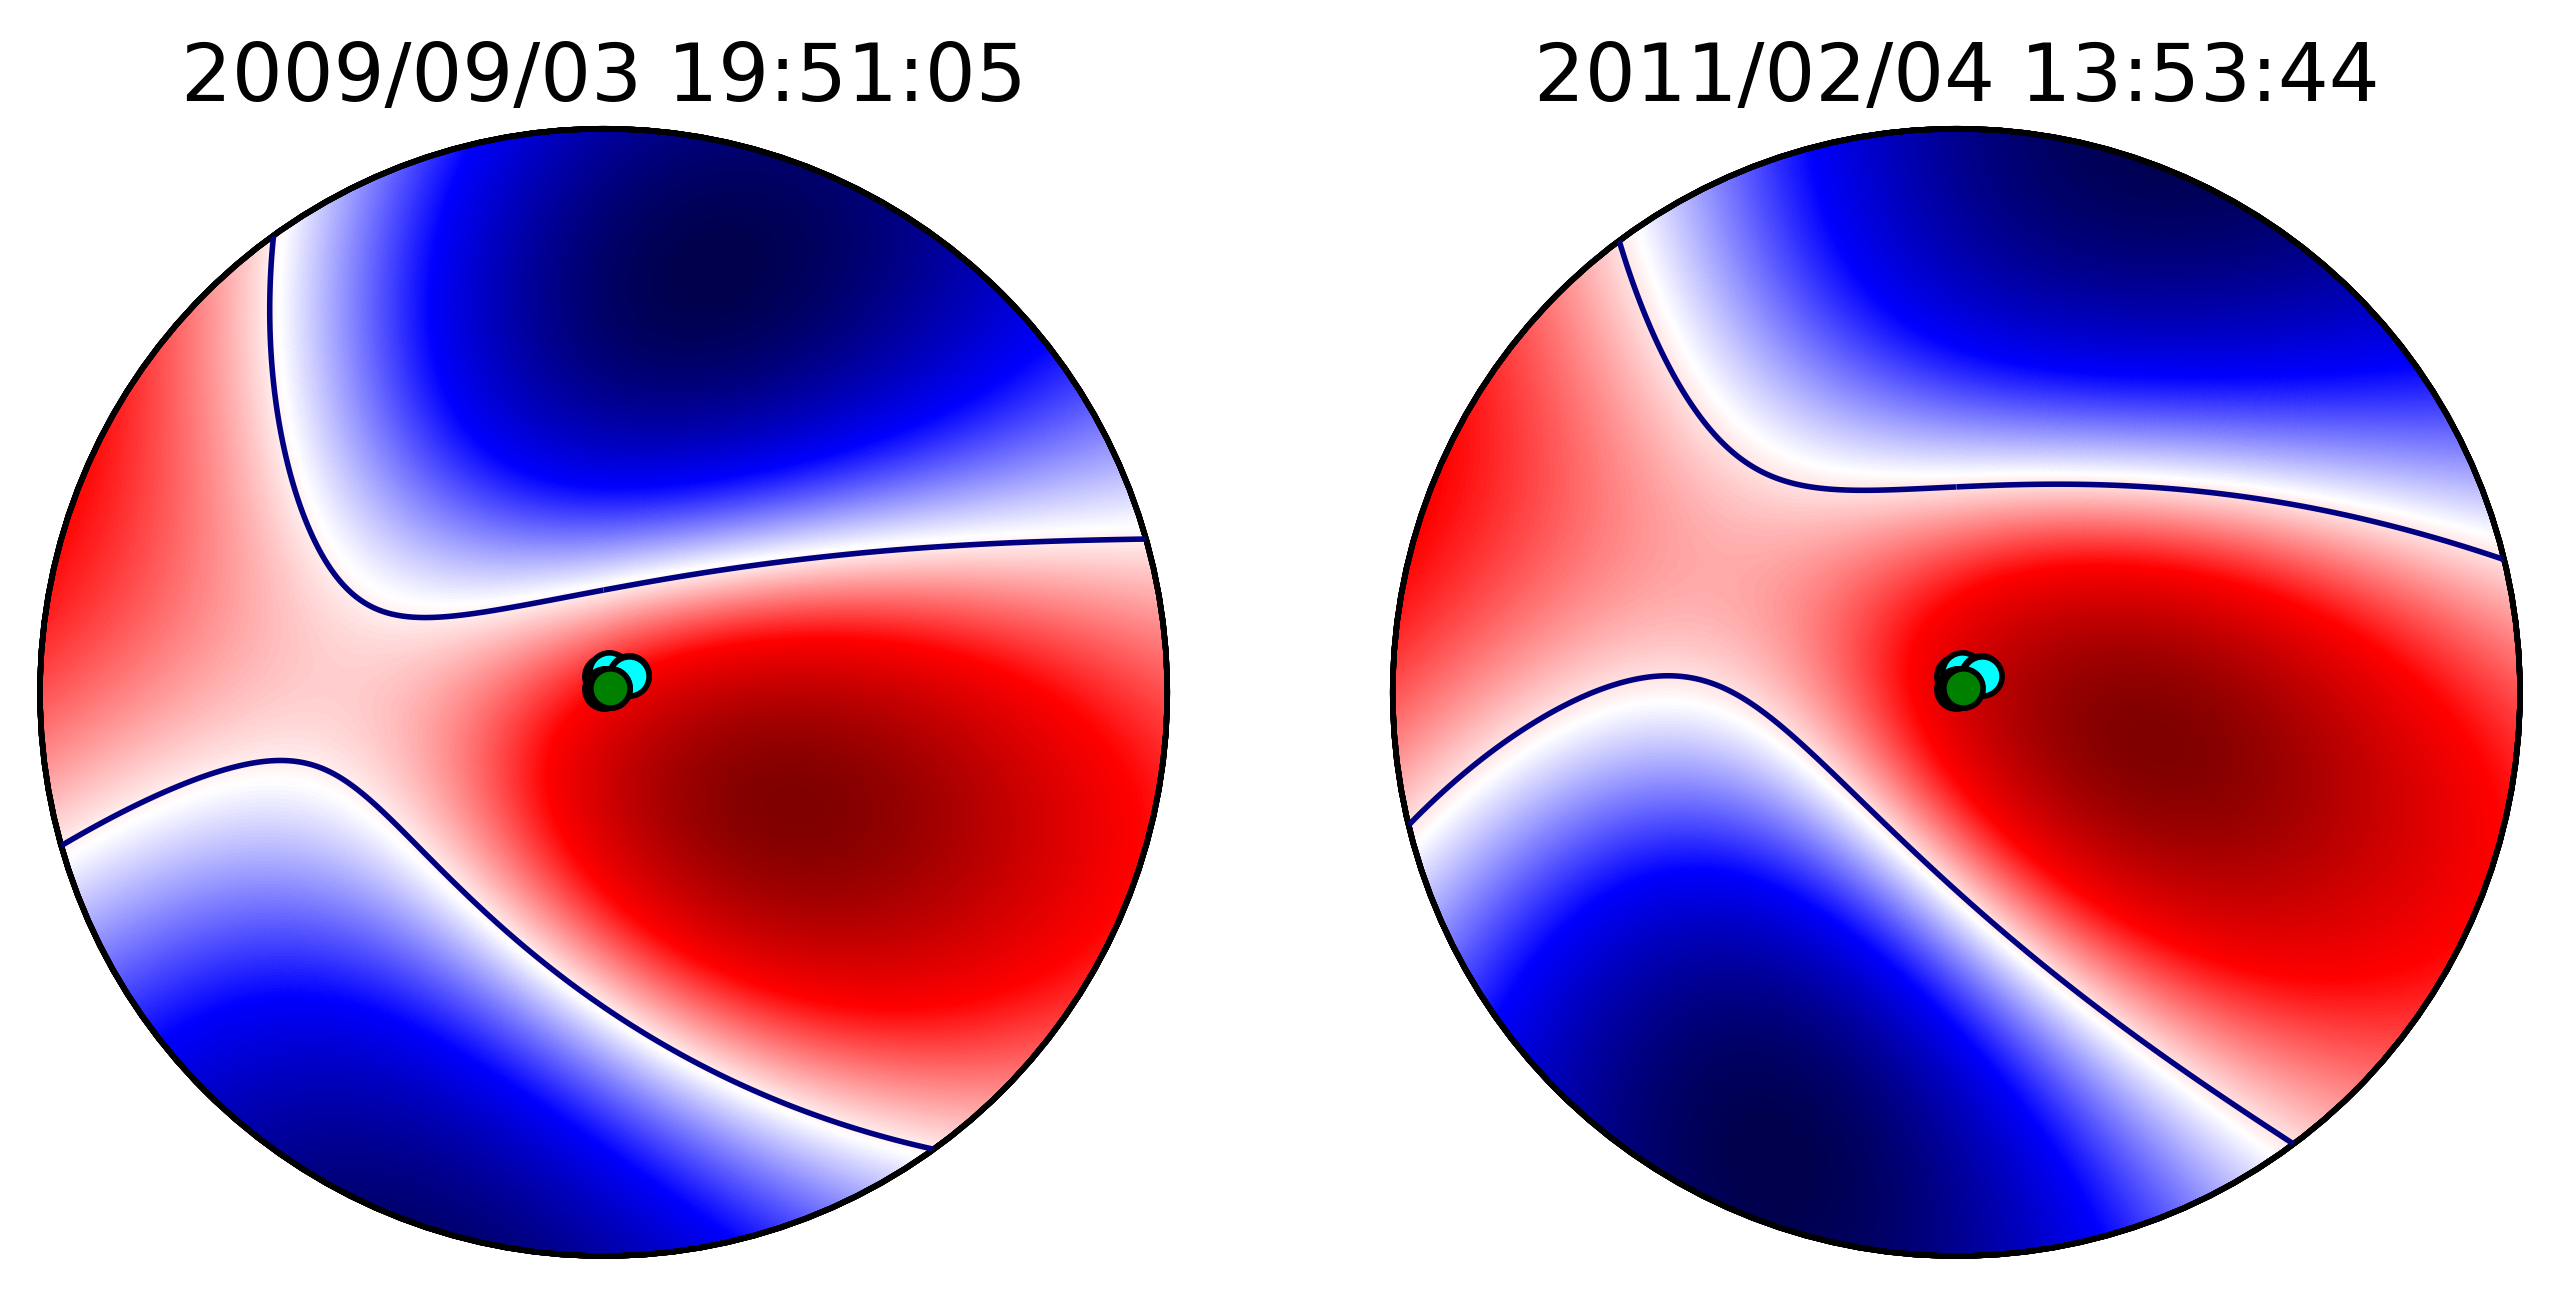
\includegraphics[width=0.68\linewidth]{fig/chap4/mt.png}
\caption{表\ref{repeat_obs}中两个地震的震源机制,浅蓝色圆圈对应PcP的出射位置,绿色圆圈对应PKiKP的出射位置.}
\label{fig:mt}
\end{figure}

\begin{figure}[ht]
\centering
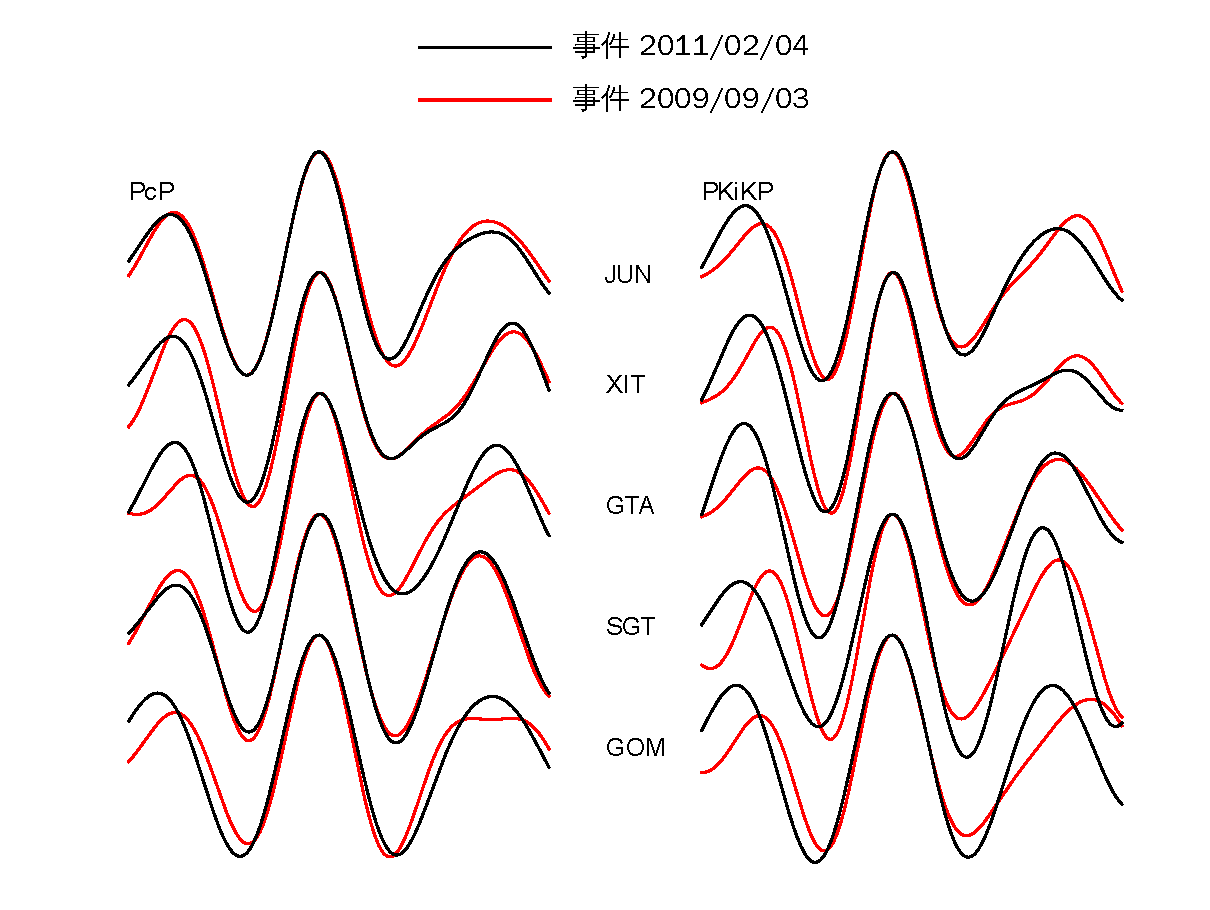
\includegraphics[width=0.8\linewidth]{fig/chap4/doublet_m}
\caption{表\ref{repeat_obs}中五个台站对两个地震的PcP和PKiKP记录,红色表示2009年的事件的波形,黑线表示2011年事件的波形. 对于2009年的事件,PcP和PKiKP的波形均做了倒转.}
\label{fig:doublet_m}
\end{figure}

通过比较同一个台站的两次记录,2009年地震的PKiKP/PcP对数振幅残差整体比2011年稍大,但差异也不是特别
显著,即两个地震的LARR同时接近零或同时偏大,这也说明对2011年地震PKiKP/PcP振幅比的观测还是比较可靠
的. 相比振幅观测的不稳定性,两个事件的PKiKP-PcP走时残差的观测则相当一致,单个台站的差别最多也只达到
几个采样间隔,这也体现出即使内核存在差异旋转,CMB和ICB也不存在可观测到的随时间变化的界面起伏变化. 因此这里认
为,造成单台站振幅比观测不稳定的因素主要有两个:(1)台站的信噪比;(2)地震的震级. 关于震级会影响PKiKP/PcP振幅比的观测结果,之前并没有研究提到过. 因为不论是CMB还是ICB,它们都不是理想的线弹性介质,反射波的振幅与入射波能量的大小也并不一定是线性关系,这也体现出使用PKiKP/PcP振幅比来约束CMB或者ICB结构方法上的缺陷.

\chapter{总结与展望}

本硕士论文结合PcP和PKiKP数据对地球核幔边界(CMB)结构变化进行研究,包括CMB的界面起伏和其上方的低速结构. 并通过一些实际的例子,分析了CMB结构变化对PKiKP/PcP振幅比和PKiKP-PcP走时残差观测的影响. 

首先利用IMS小口径台阵数据分析了CMB的小尺度起伏变化和超低速带对PKiKP/PcP振幅比观测的影响:(1) 通过NVAR和PDAR对同一地震事件的PcP和PKiKP记录比较,并结合之前波形模拟~\citep{Wu2014a}的结果,推断出CMB上可能存在局部的上凸,造成采样到不同区域的短周期PcP振幅和波形的变化;(2) 基于\citet{Rost2004a}对采样阿拉斯加Kenai半岛下方CMB被异常放大的PcP的观测,本研究结合PcP和PKiKP振幅比观测,也发现采样到Kenai半岛下方的区域的PKiKP和PcP的振幅比明显偏小,同时观察到振幅比和走时残差存在明显的相关性,从而进一步验证了前人研究的结果,即Kenai半岛下方存在局部CMB凹陷,放大了PcP振幅;(3) 通过对采样到之前研究中已经确认的澳大利亚太平洋西海岸一侧下方CMB的超低速带(ULVZ)结构~\citep{He2006a,He2012a,Thorne2004a}的WAR和ASAR数据进行分析,发现了该区域存在普遍为PREM理论值1--2倍的PKiKP/PcP振幅比,这恰好可以用之前研究得出的15\%左右的S波波速降低来解释,结合走时残差的分析,得出该CMB区域并不存在明显的界面起伏变化,从而进一步检验了CMB低速结构对PKiKP/PcP振幅比观测的影响. 

除了小口径台阵数据,本研究还利用国家测震台网观测到的PKiKP和PcP数据对位于东亚的中国下方的CMB结构变化进行分析. 通过比较筛选出的高质量PKiKP和PcP数据的振幅比和走时残差,发现与Kenai半岛的例子相似,二者存在明显的正相关性,即高的振幅比对应小的负走时残差,而低振幅比则相反. 在排除其他可能的影响因素后,本研究认为中国下方的CMB存在尺度达到200至400km的界面隆升或者凹陷,而且在大范围的隆升的界面上可能还耦合了小的凹陷,造成了PKiKP/PcP振幅比对数残差显示出负异常被正异常包围的现象. 在此观测的基础上,本文还通过对重复地震的PKiKP-PcP振幅比和走时残差观测进一步评估了观测的可靠性,并对单台站振幅比观测不确定性的主要来源进行了讨论. 

综合本研究的结果,CMB结构的各种变化均会对反射的PcP造成显著的影响,从而造成PKiKP-PcP振幅比和走时观测的区域性离散. 因此用这PcP和PKiKP研究内核外核边界结构仍然需要保持谨慎,否则将很难得到关于ICB的真实信息. 即使考虑到CMB的复杂性,单纯利用振幅比和走时残差的方法也不容易将CMB各种效应定量的分离出来. 若要得到对ICB或者CMB结构更强的约束,则需要挖掘波形中更多的信息. 目前已经有一些尝试,比如利用PKiKP和PcP谱比的方法~\citep{Tanaka2015a},利用更先进的波形模拟技术或者全波形反演方法~\citep{Fichtner2009}也可能是今后CMB或ICB结构研究的发展方向. 另外,将地震学反演和地球动力学模拟结合起来也有助于CMB复杂结构形成机制的阐明~\citep{Steinberger2008a,Soldati2012a}.

\chapter*{致谢}

有很多话要说,但摄于文字力的持久,我努力克制自己的妄言. 三年的硕士研究生学习即将结束,而我有太多需
要感谢的人. 

首先,我要感谢艾印双老师对我在学术上的指导以及生活上无微不至的关怀. 艾老师尽可能地为我们创造良好的学
习环境,勉励我不断上进. 艾老师虽然研究任务繁忙,同时身负课题组众多事务,但还是经常抽出时间和我探讨问题,给了我很多启发. 在生活上,艾老师也时时教导我做人做事的道理,让我备受感动. 如果没有艾老师的悉心指导,我是难以完成硕士论文的. 

我要感谢课题组的老师们. 郑天愉老师、何玉梅老师、赵亮老师、陈棋福老师、姜明明老师和吕彦老师,他们作为我硕士论文开题和中期报告考核小组的成员,给我的工作提了很好的意见,他们的教导都对我产生了很大的帮助. 其中,郑老师求实的治学风格给我留下了深刻的印象,她对我的鼓励是我前进的巨大动力;还有陈凌老师,每次请她帮忙,她总是不厌其烦. 虽然陈老师工作繁忙,平时我和她的交流不多,但她对我的教诲当永远不会忘记. 

我要感谢教育处的宋玉环老师、李铁胜老师和黄莹老师. 他们深刻了解学生们的学习和科研压力,经常组织我们参加各种户外活动,让我们放松身心,从而更好地投身于科研工作. 这里要特别感谢宋玉环老师,为我在去年申请到日本交流的过程中提供了很大帮助,没有她的帮忙,我必定是不能顺利成行的. 

我要感谢课题组的同学们:王旭、王武、陈瑛、魏晓拙、张耀阳师兄、徐小兵师兄、凌媛师姐还有申中寅师兄,大家
共同营造了一个团结和谐的学习环境. 其中最需要感谢的是申中寅师兄对我在学习上的帮助和研究上的鼓励. 正是申
师兄的鼓励给在处于困境中的我带来了希望,让我克服了研究工作中的重重困难,他就像黑暗中的灯塔,照亮我前进
的方向. 不仅如此,申师兄的睿智也时刻给我带来无限的启迪,这也让我对他充满了敬仰之情. 另外,我还要特别感
谢魏晓拙师弟. 他活泼开朗,谈笑风声,与他的交流总是让我感到非常愉快,让我在枯燥的科研工作中感到了不少欢
乐,支持着我度过艰难的日子. 

我还要感谢钮凤林老师,感谢他百忙之中抽出时间来听我的工作汇报. 虽然是几句不经意间的建议,却给我的研究工
作带来了很大的帮助. 通过和他的交流,可以看出他总能站在高处看待科学问题,不愧是有大家风范. 除此之外,我
还要感谢东京大学地震研究所的川勝教授,虽然只和他在去年有短短十几天的交流,但他对待科学严谨的态度给我留
下了深刻的印象,在对问题的分析方法上给了我很大启发,也正是在那之后,我的研究工作有了新的进展. 今后的研究之路上还要希望他继续指导. 

本硕士论文中理论PKiKP/PcP振幅比计算用到了Jaromir Jansky的动态射线追踪程序zrayamp~(\url{http://www.spice-rtn.org/library/software/Raytheory.html});数据处理工作用到了SAC~\citep{Goldstein2003a}和ObsPy~\citep{Beyreuther2010a},它们为本研究工作带来了极大的方便;本论文中涉及到的走时计算使用到Taup~\citep{Crotwell1999a};作图使用到了GMT~\citep{Wessel1991a}和Matplotlib~\citep{Hunter2007a},在此感谢这些软件的开发者们. 

最后,还要感谢IRIS数据中心和国家测震台网数据备份中心为本硕士论文研究提供数据支持.

\backmatter


\bibliographystyle{apalike}
\bibliography{seis}

\chapter*{待发表文章目录}

\vspace{30pt}

\textbf{\songti 龙鑫},艾印双. 基于全球小口径地震台阵的PcP和PKiKP震相研究. 地球物理学进展,2016,已录用.
\end{document}